\documentclass[12pt,a4paper]{article}

% -------------------------------------------------
% PAQUETES
% -------------------------------------------------
\usepackage[utf8]{inputenc}
\usepackage[T1]{fontenc}
\usepackage[spanish,es-nodecimaldot]{babel}
\usepackage{geometry}
\usepackage{graphicx}
\usepackage{pdflscape}
\usepackage{booktabs}
\usepackage{array}
\usepackage{longtable}
\usepackage{float}
\usepackage{needspace}
\usepackage{enumitem}
\usepackage{hyperref}
\usepackage{xurl}
\usepackage[protrusion=true,expansion=false]{microtype}
\usepackage{xcolor}
\usepackage{fancyhdr}

\geometry{
    top=2.5cm,
    bottom=2.5cm,
    left=2.5cm,
    right=2.5cm
}

\hypersetup{
    colorlinks=true,
    linkcolor=black,
    urlcolor=blue,
    citecolor=black
}

\setlength{\parindent}{0pt}
\setlength{\parskip}{0.7em}
\setlength{\emergencystretch}{2em}

% Configuración de encabezado/pie para la carátula
\fancyhf{}
\renewcommand{\headrulewidth}{0pt}
\renewcommand{\footrulewidth}{0pt}


% Presentacion unificada de figuras y codigos SQL
% Las figuras y tablas llevan sus leyendas debajo. La atribucion a fuentes externas se cita en el cuerpo del informe.
\usepackage{caption}
\captionsetup[figure]{position=bottom,font=small,labelfont=bf,
    justification=centering,singlelinecheck=false,skip=6pt}
\captionsetup[table]{position=bottom,font=small,labelfont=bf,
    justification=centering,singlelinecheck=false,skip=6pt}

\usepackage{listings}
\usepackage{upquote}
\usepackage[most]{tcolorbox}
\lstdefinestyle{sqlproyecto}{
    language=SQL,
    basicstyle=\ttfamily\scriptsize,
    keywordstyle=\bfseries\color{violet!75!black},
    commentstyle=\itshape\color{green!45!black},
    stringstyle=\color{orange!65!black},
    numberstyle=\tiny\color{black!55},
    numbers=left,
    numbersep=10pt,
    stepnumber=1,
    breaklines=true,
    breakatwhitespace=false,
    columns=fullflexible,
    keepspaces=true,
    showstringspaces=false,
    tabsize=2,
    xleftmargin=20pt,
    xrightmargin=0pt,
    frame=none,
    aboveskip=0pt,
    belowskip=0pt
}
% Numeracion correlativa de los bloques y encabezado oscuro, en estilo uniforme.
% El marco es divisible cuando un fragmento SQL excede una pagina.
\newtcblisting[auto counter]{sqlbloque}[2][]{%
    enhanced,breakable,listing only,listing engine=listings,
    listing options={style=sqlproyecto},
    colback=black!2,colframe=black!50,
    colbacktitle=black!72,coltitle=white,
    fonttitle=\small\bfseries,
    title={Bloque de código \thetcbcounter: #2},
    left=4.5mm,right=1.5mm,top=1mm,bottom=1mm,
    boxrule=0.55pt,arc=1mm,
    before skip=9pt,after skip=9pt,
    attach boxed title to top left={xshift=0mm,yshift=0mm},
    #1
}
% Comparaciones de planes obtenidos en pgAdmin mediante EXPLAIN ANALYZE.
% Se muestran extractos vectoriales de nodos relevantes para preservar legibilidad.
% Los diez SVG íntegros se conservan sin modificaciones como evidencia técnica.
\newcommand{\plancomparativo}[2]{%
  \begin{figure}[H]
  \centering
  \vspace{3pt}
  {\small\bfseries (a) Sin índices secundarios experimentales}\par\vspace{3pt}
  \includegraphics[width=0.97\linewidth,height=0.28\textheight,keepaspectratio]{figuras/plan_#1_sin_extracto.pdf}\par
  \vspace{7pt}
  {\small\bfseries (b) Con índices candidatos disponibles}\par\vspace{3pt}
  \includegraphics[width=0.97\linewidth,height=0.28\textheight,keepaspectratio]{figuras/plan_#1_con_extracto.pdf}
  \caption{Consulta #2: extractos de los planes de ejecución, sin índices secundarios y con índices candidatos (un millón de registros).}
  \label{fig:plan-#1-comparacion}
  \end{figure}%
}

% Apéndice documental de integradores SQL.
\lstdefinestyle{sqlanexo}{
    language=SQL,
    basicstyle=\ttfamily\fontsize{7.4}{9.0}\selectfont,
    keywordstyle=\bfseries\color{violet!65!black},
    commentstyle=\color{green!40!black},
    stringstyle=\color{orange!60!black},
    numbers=left,
    numberstyle=\ttfamily\fontsize{6.4}{8}\selectfont\color{black!45},
    numbersep=7pt,
    stepnumber=5,
    breaklines=true,
    breakatwhitespace=false,
    columns=fullflexible,
    keepspaces=true,
    showstringspaces=false,
    tabsize=2,
    xleftmargin=2.2em,
    xrightmargin=0.5em,
    frame=single,
    framesep=4pt,
    rulecolor=\color{black!24},
    backgroundcolor=\color{black!1},
    aboveskip=7pt,
    belowskip=9pt,
    captionpos=b,
    inputencoding=utf8,
    literate={é}{{\'e}}1 {á}{{\'a}}1 {í}{{\'i}}1 {ó}{{\'o}}1 {ú}{{\'u}}1 {ñ}{{\~n}}1
}

\begin{document}
\hypersetup{pageanchor=false}
\begin{titlepage}
\thispagestyle{fancy}
\begin{center}

\vspace*{0.5cm}


\includegraphics[width=0.37\textwidth]{isologo-utec.png}\\[0.8cm]

{\Large \textbf{Base de Datos I (CS2041)}}\\[0.2cm]
{\large 2026-2}\\[1.0cm]

{\large \textbf{Proyecto Final}}\\[0.5cm]

{\Large \textbf{Sistema de Monitoreo Sismológico y Alerta Temprana}}\\[1.3cm]

{\large
\textbf{Profesor a cargo:} Wilder Nina\\[0.70cm]
}

{\large \textbf{Integrantes}}\\[0.45cm]

\begin{tabular}{l c}
\hline\\[-0.2cm]
Chala Lastra, Jared Eloy Daniel & 202520040\\[0.25cm]
Landeo Huatay, Leonard Alexander & 202520151\\[0.25cm]
Tumialan Maihua, Fabricio Nick & 202520045\\
\end{tabular}

\vfill

{\large \textbf{2026}}\\[0.35cm]
{\large Lima, Perú}

\end{center}
\end{titlepage}
\hypersetup{pageanchor=true}

\tableofcontents
\newpage

% =================================================
% 1. REQUISITOS
% =================================================

\section{Requisitos}

% -------------------------------------------------
% 1.1
% -------------------------------------------------

\subsection{Introducción}

El presente proyecto desarrolla el diseño y la implementación de una base de datos relacional para el monitoreo sismológico y la gestión de alertas tempranas. Su estructura integra información de estaciones sísmicas, sensores, lecturas instrumentales, eventos sísmicos, detecciones y alertas emitidas.

La propuesta busca representar de manera estructurada el flujo de información generado durante el monitoreo de la actividad sísmica, permitiendo relacionar cada estación con sus respectivos sensores, conservar las mediciones obtenidas, registrar las características principales de los eventos sísmicos y mantener un historial de las alertas asociadas a dichos eventos.

A partir del análisis de la información se definieron el modelo conceptual y el modelo relacional, con las entidades, relaciones y restricciones necesarias para representar el dominio. Ambos modelos sustentan la implementación del esquema en PostgreSQL y las consultas utilizadas para su evaluación.

% -------------------------------------------------
% 1.2
% -------------------------------------------------

\subsection{Descripción general del problema/organización/empresa}

El monitoreo sismológico requiere recopilar y administrar información proveniente de múltiples estaciones distribuidas geográficamente. Estas estaciones contienen sensores encargados de registrar el movimiento del suelo y producir mediciones que posteriormente pueden ser utilizadas para identificar y analizar eventos sísmicos.

Para el desarrollo del proyecto se plantea una organización ficticia encargada del monitoreo sísmico, cuya función es administrar una red de estaciones y sensores, conservar las mediciones generadas por estos dispositivos, registrar los eventos sísmicos identificados y mantener información sobre las alertas asociadas a dichos eventos.

El principal problema consiste en gestionar de manera consistente información de distinta naturaleza pero estrechamente relacionada. La organización necesita poder determinar, por ejemplo, qué sensores participaron en la detección de un evento, a qué estaciones pertenecen dichos sensores, qué características presenta el evento registrado y qué alertas fueron generadas a partir de este. Por ello, se requiere una estructura de datos que permita integrar y relacionar esta información de forma organizada.

% -------------------------------------------------
% 1.3
% -------------------------------------------------

\subsection{Necesidad/usos de la base de datos}
La organización requiere una base de datos que permita centralizar y relacionar la información generada durante el monitoreo sismológico. Debido a que los datos corresponden a distintos objetos, como estaciones, sensores, lecturas, eventos sísmicos y alertas, resulta necesario mantener una estructura que permita conservar sus relaciones y garantizar la consistencia de la información almacenada.

La base de datos permitirá mantener un registro histórico de las mediciones generadas por los sensores, identificar qué dispositivos y estaciones participaron en la detección de un determinado evento sísmico y conservar las características asociadas a cada evento. Asimismo, permitirá registrar las alertas vinculadas a estos eventos y mantener información sobre su emisión y estado.

Además de facilitar el registro y recuperación de información, la base de datos servirá como soporte para consultas operativas e históricas, así como para la generación de estadísticas sobre la actividad sísmica registrada. La centralización de los datos también permitirá reducir la duplicidad de información, facilitar su actualización y establecer restricciones que mantengan la integridad de los registros.
% -------------------------------------------------
% 1.4
% -------------------------------------------------

\subsection{¿Cómo se resuelve el problema hoy?}

Para efectos del proyecto, se asume que la organización gestiona actualmente la información mediante archivos independientes y herramientas de almacenamiento no integradas. Los datos correspondientes a estaciones, sensores, lecturas, eventos sísmicos y alertas se mantienen en fuentes separadas y deben ser relacionados posteriormente cuando se requiere realizar una consulta que involucre más de un tipo de información.

Este esquema puede resultar suficiente mientras el volumen de datos es reducido; sin embargo, a medida que aumenta la cantidad de estaciones, sensores y mediciones registradas, se vuelve más difícil mantener la información consistente y realizar consultas de manera eficiente. La ausencia de una estructura centralizada también incrementa el riesgo de duplicidad, inconsistencias y errores durante la búsqueda o actualización de los datos.

 

% -------------------------------------------------
% 1.4.1
% -------------------------------------------------

\subsubsection{¿Cómo se almacenan/procesan los datos hoy?}

Se asume que la información de las estaciones y sensores se mantiene principalmente en hojas de cálculo, mientras que las mediciones generadas por los sensores se almacenan en archivos CSV debido a su naturaleza tabular y a su mayor volumen. Por otra parte, los eventos sísmicos identificados y las alertas emitidas se conservan en reportes independientes.

Debido a esta separación, las operaciones que requieren combinar información de distintos objetos deben realizarse mediante búsquedas y cruces manuales entre varios archivos. Este procedimiento puede implicar comparar identificadores, fechas, horas y otros atributos para determinar qué registros se encuentran relacionados.

Por ejemplo, para responder a la consulta ``¿qué sensores detectaron un determinado evento sísmico y con qué aceleración máxima?'', un operador tendría que localizar primero el evento en el registro correspondiente, revisar los datos disponibles de los sensores dentro del intervalo temporal asociado al evento y, posteriormente, consultar la información de cada sensor para determinar la estación a la que pertenece.

A medida que aumenta el número de sensores y lecturas registradas, este procedimiento requiere mayor tiempo y aumenta la posibilidad de errores, como omitir registros relevantes, relacionar datos incorrectos o mantener versiones inconsistentes de la misma información. Estas limitaciones justifican la necesidad de sustituir el manejo fragmentado de los datos por una estructura relacional centralizada.

 

% -------------------------------------------------
% 1.4.2
% -------------------------------------------------

\subsubsection{Flujo de datos}

El flujo de información del sistema comienza en las estaciones sísmicas, donde se encuentran instalados los sensores encargados de registrar el movimiento del suelo. Cada sensor genera lecturas de manera periódica o continua de acuerdo con su frecuencia de muestreo, y cada una de estas mediciones queda asociada al dispositivo que la produjo.

Las lecturas generadas constituyen la información instrumental utilizada durante el monitoreo. Cuando se identifica un evento sísmico, se registra un único evento con sus principales características, como fecha y hora de origen, ubicación aproximada del epicentro, profundidad y magnitud.

Debido a que un mismo evento puede ser observado por sensores pertenecientes a distintas estaciones, el sistema registra individualmente la participación de cada sensor mediante una detección. Cada detección relaciona un sensor con el evento sísmico correspondiente y puede conservar información específica del registro, como la hora de detección, la aceleración máxima observada y un indicador de calidad.

De esta manera, varios sensores pueden encontrarse asociados a un mismo evento sin duplicar la información general de este. Asimismo, un mismo sensor puede participar en la detección de múltiples eventos a lo largo del tiempo.

Finalmente, cuando un evento cumple con los criterios establecidos para la emisión de una alerta, se registra una alerta asociada a dicho evento. Esta puede almacenar información como la fecha y hora de emisión, el nivel asignado, el mensaje, la magnitud estimada al momento de su emisión y su estado.

De manera general, el flujo de información se representa en la Figura \ref{fig:flujo-datos}.

\begin{figure}[H]
    \centering
    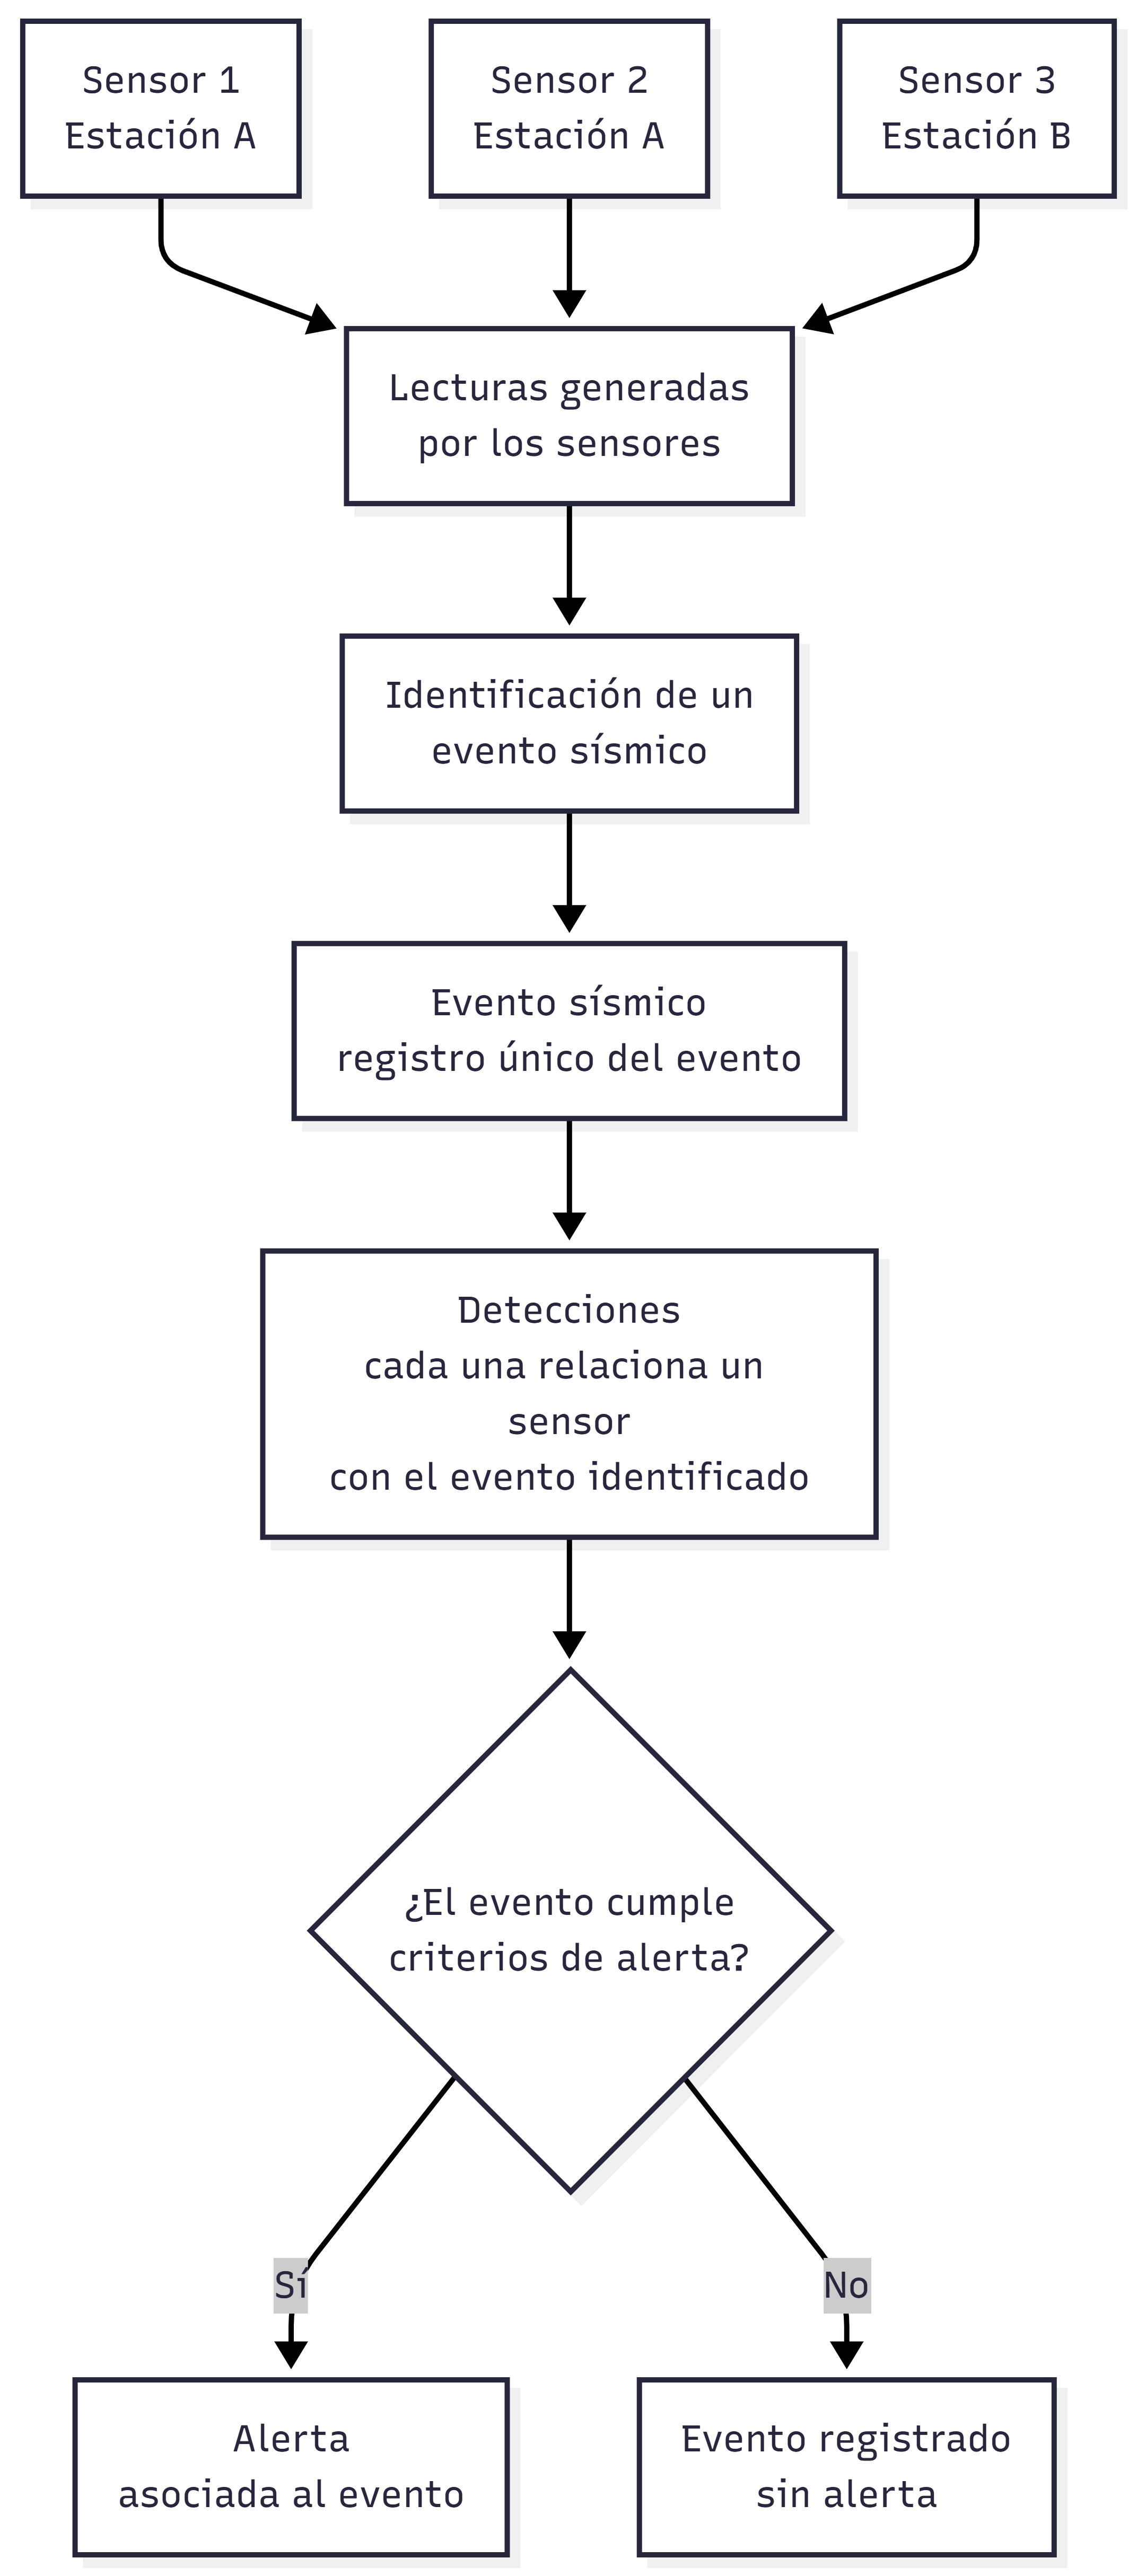
\includegraphics[width=0.60\textwidth]{figuras/flujo_de_datos_proyecto.png}
    \caption{Flujo general de datos del sistema de monitoreo sismológico y alerta temprana.}
    \label{fig:flujo-datos}
\end{figure}

El flujo descrito corresponde al proceso esperado del sistema, no a un mecanismo de detección automatizada ya implementado. Se distingue del manejo actual por archivos independientes. La siguiente tabla vincula las dificultades de dicho manejo con las funcionalidades que debe resolver la base de datos.

\begin{table}[H]
\centering
\small
\begin{tabular}{>{\raggedright\arraybackslash}p{3.9cm} >{\raggedright\arraybackslash}p{6.2cm} >{\raggedright\arraybackslash}p{3.0cm}}
\toprule
\textbf{Situación asumida actualmente} & \textbf{Problema que debe resolver la base de datos} & \textbf{Requerimientos} \\
\midrule
Estaciones y sensores en hojas de cálculo separadas. & Evitar referencias inconsistentes y duplicación de identificadores, conservando la instalación actual de cada sensor. & RF--01, RF--02 \\
Lecturas almacenadas en archivos CSV independientes. & Recuperar registros por sensor y período, evitar duplicaciones y conservar la marca de validez sin eliminar mediciones. & RF--04, RF--05, RF--09 \\
Eventos, detecciones y alertas conservados en reportes distintos. & Vincular los sensores participantes con eventos y alertas mediante identificadores consistentes, facilitando consultas históricas. & RF--06 a RF--10 \\
\bottomrule
\end{tabular}
\caption{Relación entre el estado actual asumido del manejo de datos y las funcionalidades previstas.}
\end{table}


 

% -------------------------------------------------
% 1.5
% -------------------------------------------------

\subsection{Descripción detallada del sistema}

El sistema propuesto tiene como finalidad gestionar de forma centralizada la información generada durante el monitoreo sismológico. Para ello, integra los datos correspondientes a estaciones sísmicas, sensores, lecturas, eventos sísmicos, detecciones y alertas, manteniendo las relaciones necesarias entre estos elementos.

La información almacenada presenta diferentes características y frecuencias de actualización. Mientras que los datos de estaciones y sensores corresponden principalmente a información estructural y operativa, las lecturas son generadas de manera continua o periódica y constituyen el mayor volumen de registros. Por su parte, los eventos sísmicos, las detecciones y las alertas se incorporan cuando se identifican situaciones asociadas a la actividad sísmica monitoreada.

A partir de esta estructura, el sistema deberá permitir tanto operaciones de registro y actualización como consultas operativas, históricas y analíticas, manteniendo la consistencia e integridad de la información almacenada.

% -------------------------------------------------
% 1.5.1
% -------------------------------------------------

\subsubsection{Objetos de información actuales}

Para efectos del proyecto, se identifican como objetos de información aquellos elementos del dominio que deben ser registrados, relacionados o consultados durante el monitoreo sismológico y la gestión de alertas. Cada uno representa información con un significado específico dentro del sistema.

\begin{longtable}{p{3.5cm} p{10cm}}
\toprule
\textbf{Objeto} & \textbf{Descripción} \\
\midrule
\endfirsthead

\toprule
\textbf{Objeto} & \textbf{Descripción} \\
\midrule
\endhead

\textbf{Estación sísmica} &
Punto físico de monitoreo ubicado en una determinada zona geográfica. Almacena información de identificación, ubicación, fecha de instalación y estado operativo. \\[0.3cm]

\textbf{Sensor} &
Dispositivo instalado en una estación sísmica y encargado de registrar el movimiento del suelo. Contiene información sobre su identificación, características técnicas, frecuencia de muestreo, fecha de instalación, fecha del último mantenimiento y estado operativo. \\[0.3cm]

\textbf{Lectura de onda} &
Medición individual generada por un sensor en un instante determinado. Permite conservar el valor registrado, la información temporal asociada a la medición y un indicador que señale si la lectura fue considerada válida después de su revisión. \\[0.3cm]

\textbf{Evento sísmico} &
Registro de un sismo identificado dentro del sistema. Contiene sus principales características, como fecha y hora de origen, ubicación del epicentro, profundidad, magnitud y referencia geográfica. \\[0.3cm]

\textbf{Detección} &
Asociación que representa la participación de un sensor específico en el registro de un evento sísmico determinado. Puede conservar información propia de dicha detección, como la hora de registro, la aceleración máxima observada y un indicador de calidad. \\[0.3cm]

\textbf{Alerta} &
Registro informativo generado a partir de un evento sísmico cuando corresponde. Incluye información como fecha y hora de emisión, nivel, mensaje, magnitud estimada y estado. \\

\bottomrule
\end{longtable}

Estos objetos de información constituyen la base del diseño conceptual del sistema. En el modelo Entidad--Relación se determinará cuáles serán representados como entidades y cuáles mediante relaciones, junto con sus atributos, multiplicidades y restricciones de participación.

% -------------------------------------------------
% 1.5.2
% -------------------------------------------------

\subsubsection{Características y funcionalidades esperadas}

El sistema deberá permitir gestionar de manera centralizada la información relacionada con el monitoreo sismológico, manteniendo relaciones consistentes entre estaciones sísmicas, sensores, lecturas, eventos, detecciones y alertas.

Con base en las reglas semánticas de la Sección 2.1, los requerimientos funcionales se especifican de forma verificable a continuación. Los códigos RF permiten identificar qué operación debe satisfacer la implementación y qué restricciones deben comprobarse. La identificación de los actores se corresponde con los perfiles descritos en la siguiente sección.

\begin{longtable}{>{\raggedright\arraybackslash}p{1.65cm} >{\raggedright\arraybackslash}p{10.5cm} >{\raggedright\arraybackslash}p{2.1cm}}
\toprule
\textbf{Código} & \textbf{Requerimiento funcional y condición de cumplimiento} & \textbf{Reglas} \\
\midrule
\endfirsthead
\toprule
\textbf{Código} & \textbf{Requerimiento funcional y condición de cumplimiento} & \textbf{Reglas} \\
\midrule
\endhead
RF--01 & El administrador registra y actualiza estaciones con identificador y código no repetidos. Toda estación registrada debe quedar asociada por lo menos a un sensor, conforme al alcance del modelo. & 1--3 \\
RF--02 & El administrador registra y actualiza sensores asociados a una sola estación, sin repetir identificador ni número de serie. Se conserva la instalación actual, sin historial de traslados. & 3--5, 26 \\
RF--03 & El administrador registra los cambios de estado y la última fecha de mantenimiento de cada sensor. Esta fecha puede ser nula; cuando exista, debe ser igual o posterior a la fecha de instalación. & 6--8, 25 \\
RF--04 & El proceso de captura incorpora lecturas con sensor existente, fecha y hora, canal, valor y validez. No se duplica la combinación de sensor, instante y canal. & 9--11, 26 \\
RF--05 & El operador puede marcar lecturas como no válidas sin eliminarlas. La admisión de nuevas lecturas válidas para el análisis considera el estado operativo del sensor al momento de registrarlas. & 12--13, 24 \\
RF--06 & El operador registra y actualiza eventos sísmicos con fecha y hora de origen, epicentro, profundidad y magnitud, respetando los dominios definidos. & 14, 22--23 \\
RF--07 & El operador registra la detección de un evento por un sensor, con hora, aceleración máxima y calidad, sin repetir la pareja sensor--evento. Se admite que existan sensores sin detecciones y eventos sin detecciones. & 15--19 \\
RF--08 & El operador registra las alertas emitidas, sus niveles, mensajes y estados. Cada alerta se asocia a un evento existente y un evento puede no generar alertas o generar varias. & 20--21, 26 \\
RF--09 & Los usuarios autorizados pueden consultar estados, mantenimientos, lecturas por intervalo, eventos por identificador y alertas. El alcance de lectura o actualización depende del perfil de usuario. & 25--26 \\
RF--10 & Los analistas pueden ejecutar consultas de detecciones por evento, conteo de eventos por estación, promedios de aceleración, sensores sin lecturas y actividad histórica por sensor. & 9, 15--19 \\
\bottomrule
\end{longtable}

\noindent
\textbf{Condiciones de integridad y alcance.} Las llaves primarias y foráneas, los dominios numéricos, la unicidad y las participaciones obligatorias se derivan de las reglas semánticas y del modelo relacional. La existencia de al menos un sensor por estación requiere control adicional durante el registro conjunto; una llave foránea en \texttt{SENSOR} no garantiza por sí sola esta condición. Los mecanismos concretos se definirán en la implementación de procedimientos y disparadores. El sistema conserva registros de alertas, pero no implementa su difusión física o pública.

\noindent
\textbf{Frecuencia de operación.} Estaciones y sensores se incorporan o modifican de manera ocasional; lecturas se cargan de manera continua o periódica; eventos, detecciones y alertas se registran cuando ocurre una identificación o emisión. Esta diferencia justifica la prioridad de carga y consulta sobre \texttt{LECTURA\_\allowbreak{}ONDA} y \texttt{DETECCION} al realizar las pruebas de rendimiento.

% -------------------------------------------------
% 1.5.3
% -------------------------------------------------

\subsubsection{Tipos de usuarios existentes/necesarios}

El sistema contempla distintos perfiles de usuario de acuerdo con las operaciones que realizan sobre la información almacenada y el nivel de acceso que requieren. La diferenciación de estos perfiles permitirá posteriormente establecer permisos adecuados sobre las distintas operaciones de consulta, registro y actualización.

\textbf{Administrador del sistema.}
Será responsable de gestionar la información estructural y operativa del sistema, incluyendo el registro y actualización de estaciones sísmicas, sensores y sus respectivos estados. Asimismo, podrá supervisar la consistencia general de los datos y realizar operaciones de mantenimiento administrativo.

\textbf{Operador de monitoreo.}
Utilizará el sistema para consultar información relacionada con lecturas, detecciones, eventos sísmicos y alertas. También podrá registrar o actualizar información operativa cuando corresponda al proceso de monitoreo.

\textbf{Analista o investigador.}
Accederá principalmente a información histórica con el objetivo de realizar análisis sobre los eventos registrados, comparar el comportamiento de estaciones o sensores y obtener resultados estadísticos a partir de los datos almacenados.

\textbf{Usuario de consulta.}
Tendrá acceso principalmente de lectura a información de carácter informativo, como eventos sísmicos registrados, alertas emitidas y resultados generales disponibles en el sistema, sin capacidad para modificar la información estructural de la base de datos.

Además de los usuarios anteriores, el sistema considera la interacción de un \textbf{proceso automático de captura de datos}. Este no corresponde a un usuario humano, sino a un componente encargado de incorporar de manera continua o periódica las lecturas generadas por los sensores y, cuando corresponda, registrar información derivada del proceso de monitoreo.

La definición de estos perfiles permitirá establecer posteriormente diferentes niveles de acceso, evitando que todos los usuarios o procesos puedan realizar las mismas operaciones sobre la información almacenada.

% -------------------------------------------------
% 1.5.4
% -------------------------------------------------

\subsubsection{Tipos de consulta, actualizaciones}


La base de datos deberá permitir consultas operativas para recuperar información específica y consultas históricas o analíticas que relacionen varios objetos del sistema.

Entre las consultas operativas se consideran la búsqueda de un evento sísmico por su identificador, la consulta del estado actual de estaciones y sensores, la revisión de la fecha del último mantenimiento de un sensor, la identificación de lecturas marcadas como no válidas y la recuperación de las lecturas generadas por un sensor durante un intervalo de tiempo.

Como consultas de mayor nivel se plantean las siguientes:

\begin{itemize}
    \item Identificar los sensores y estaciones que participaron en la detección de un evento sísmico determinado.

    \item Determinar la cantidad de eventos sísmicos distintos detectados por cada estación durante un periodo determinado.

    \item Obtener, para cada estación, la aceleración máxima promedio registrada en las detecciones de eventos sísmicos.

    \item Identificar los sensores que no hayan generado lecturas durante un determinado número de días, con el fin de detectar posibles periodos de inactividad.

    \item Obtener, para cada sensor, la cantidad de eventos sísmicos en los que participó y la fecha de su detección más reciente.
\end{itemize}

Respecto a las actualizaciones, la información de estaciones y sensores tendrá cambios poco frecuentes, principalmente por instalación, mantenimiento o modificación de su estado operativo. Cuando se realice un mantenimiento preventivo o correctivo se actualizará la fecha del último mantenimiento del sensor. Las lecturas serán incorporadas de manera continua o periódica y constituirán el flujo de datos de mayor frecuencia; adicionalmente, podrán marcarse como válidas o no válidas cuando se detecten mediciones anómalas o errores instrumentales.

Los eventos sísmicos y sus detecciones se registrarán cuando se identifique un nuevo evento, y sus datos podrán actualizarse posteriormente si se dispone de información revisada. Las alertas se incorporarán cuando corresponda su emisión y podrán actualizarse de acuerdo con su estado.

En cuanto a las velocidades de respuesta esperadas, las consultas operativas simples, como la búsqueda de un evento sísmico por su identificador o la revisión del estado de una estación o sensor, deberán responder aproximadamente en un segundo, incluso cuando la base de datos alcance los mayores volúmenes estimados de lecturas y detecciones. Las consultas de mayor nivel, que combinan varias relaciones o recorren intervalos temporales amplios, podrán tolerar tiempos de respuesta de algunos segundos, debido a su carácter histórico o analítico y no estrictamente operativo. Estas expectativas de rendimiento serán evaluadas posteriormente mediante la experimentación con índices sobre las cinco consultas intermedias seleccionadas para el proyecto.

% -------------------------------------------------
% 1.5.5
% -------------------------------------------------

\subsubsection{Tamaño estimado de la base de datos}

El tamaño de la base de datos dependerá principalmente de la cantidad de estaciones y sensores administrados y, sobre todo, de la frecuencia con la que se registren las lecturas. Debido a que estas mediciones pueden generarse de manera continua o periódica, la relación \texttt{LECTURA\_\allowbreak{}ONDA} será la de mayor crecimiento dentro del sistema.

Para efectos del proyecto se combinan datos reales y datos sintéticos. El catálogo público del IGP aporta los eventos sísmicos, mientras que las estaciones, sensores, lecturas, detecciones y alertas operativas se representan mediante registros simulados. Las bases experimentales también utilizan datos generados de forma controlada para estudiar el rendimiento.

Como referencia, se estima el siguiente volumen de información para el dominio planteado:

\begin{table}[H]
\centering
\begin{tabular}{lr}
\toprule
\textbf{Objeto de información} & \textbf{Cantidad estimada} \\
\midrule
Estaciones sísmicas & 100 -- 500 \\
Sensores & 300 -- 1 500 \\
Eventos sísmicos & 10 000 -- 100 000 \\
Detecciones & 100 000 -- 500 000 \\
Alertas & 1 000 -- 20 000 \\
Lecturas de onda & 1 000 000 o más \\
\bottomrule
\end{tabular}
\end{table}

Estas cantidades representan una proyección de crecimiento del sistema y no describen la distribución exacta de la base utilizada en los ensayos. De manera independiente, se prepararon cuatro conjuntos experimentales con 1 000, 10 000, 100 000 y 1 000 000 de registros, como se detalla en el Capítulo~5.

El mayor volumen de datos se concentrará en las lecturas y detecciones, por lo que las consultas relacionadas con estas relaciones serán especialmente relevantes para evaluar posteriormente el rendimiento de la base de datos.

% -------------------------------------------------
% 1.6
% -------------------------------------------------

\subsection{Objetivos del proyecto}

\subsubsection*{Objetivo general}

Diseñar e implementar en PostgreSQL una base de datos relacional para gestionar la información de estaciones sísmicas, sensores, lecturas, eventos, detecciones y alertas, garantizando la coherencia de sus relaciones y restricciones de integridad.

\subsubsection*{Objetivos específicos}

\begin{itemize}
    \item Identificar los principales objetos de información, atributos y reglas semánticas presentes en el dominio del monitoreo sismológico.

    \item Diseñar un modelo Entidad--Relación que represente adecuadamente las entidades, relaciones, atributos llave, multiplicidades y restricciones de participación del sistema.

    \item Transformar el modelo conceptual en un modelo relacional normalizado, definiendo correctamente llaves primarias, llaves foráneas y restricciones de integridad.

    \item Definir los dominios y restricciones principales de los atributos mediante un diccionario de datos coherente con el modelo relacional.

    \item Implementar consultas y mecanismos de integridad en PostgreSQL y evaluar su rendimiento mediante conjuntos de datos de distinta escala.
\end{itemize}

% -------------------------------------------------
% 1.7
% -------------------------------------------------

\subsection{Referencias del proyecto}

El proyecto toma como referencia fuentes oficiales relacionadas con la actividad sísmica en el Perú, así como documentación técnica y bibliografía académica sobre diseño e implementación de bases de datos.

\begin{itemize}

    \item \textbf{Instituto Geofísico del Perú (IGP) -- Centro Sismológico Nacional (CENSIS).}

    Fuente de los datos de eventos sísmicos utilizados en la carga oficial: fecha, hora, ubicación geográfica, magnitud y profundidad.

    \url{https://censis.igp.gob.pe/repositorio/datos-sismicos}

    \item \textbf{Instituto Geofísico del Perú (IGP) -- Sistema de Alerta Sísmica Peruano (SASPe).}

    Referencia conceptual para la organización de redes de monitoreo orientadas a la detección sísmica y a la alerta temprana.

    \url{https://www.igp.gob.pe/servicios/saspe/estaciones.php}

    \item \textbf{Instituto Geofísico del Perú (IGP) -- ACELDAT-PERÚ.}

    Referencia técnica sobre estaciones, registros acelerométricos y parámetros de medición instrumental.

    \url{https://www.igp.gob.pe/servicios/aceldat-peru/reportes-registros-acelerometricos}

    \item \textbf{PostgreSQL Global Development Group -- Documentación oficial de PostgreSQL.}

    Referencia técnica para la implementación de restricciones, consultas, índices y demás componentes utilizados en PostgreSQL.

    \url{https://www.postgresql.org/docs/}

    \item \textbf{Ramakrishnan, R. y Gehrke, J. (2003).}
    \textit{Database Management Systems} (3.\textsuperscript{a} ed.). McGraw-Hill.

    Referencia teórica para el modelo Entidad--Relación, su transformación al modelo relacional y los principios de normalización e integridad de datos.

\end{itemize}

El catálogo oficial del IGP permitió incorporar 24\,289 eventos sísmicos. La información operativa no disponible públicamente se representó mediante datos sintéticos, manteniendo explícita la diferencia entre ambas procedencias.
% -------------------------------------------------
% 1.8
% -------------------------------------------------

\subsection{Eventualidades}

Durante el desarrollo del proyecto pueden presentarse dificultades relacionadas con la obtención, calidad, integración y volumen de los datos. Asimismo, es necesario establecer límites claros para mantener el alcance del sistema dentro de los objetivos del curso.
% -------------------------------------------------
% 1.8.1
% -------------------------------------------------

\subsubsection{Problemas que pudieran encontrarse en el proyecto}

Durante el desarrollo del proyecto podrían presentarse las siguientes dificultades:

\begin{itemize}

    \item \textbf{Disponibilidad limitada de datos reales:}
    las fuentes públicas pueden proporcionar información sobre eventos sísmicos, estaciones o registros instrumentales, pero no necesariamente todos los atributos y volúmenes requeridos por el modelo.

    \item \textbf{Heterogeneidad de formatos:}
    los datos obtenidos de distintas fuentes pueden encontrarse en formatos como XLSX, CSV o reportes web, por lo que será necesario realizar procesos de limpieza y transformación antes de incorporarlos a la base de datos.

    \item \textbf{Datos incompletos, inconsistentes, duplicados o erróneos:}
    algunos registros pueden contener valores faltantes, diferencias de formato, información repetida o mediciones anómalas producidas por ruido o fallas instrumentales. Por ello, será necesario establecer criterios de validación y conservar un indicador que permita distinguir las lecturas consideradas válidas de aquellas que requieren revisión.

    \item \textbf{Asociación entre mediciones y eventos:}
    puede resultar difícil determinar qué registros instrumentales corresponden a un evento sísmico determinado, especialmente cuando varios sensores generan lecturas de manera continua.

    \item \textbf{Gran volumen de información:}
    la generación frecuente de lecturas puede producir una cantidad elevada de registros y afectar el rendimiento de determinadas consultas, aspecto que deberá considerarse durante la implementación y experimentación.

    \item \textbf{Generación de datos sintéticos coherentes:}
    cuando no exista información real suficiente, será necesario generar datos simulados que respeten los dominios, restricciones y relaciones establecidas en el modelo.

\end{itemize}

Estas dificultades deberán considerarse durante la preparación, carga y validación de los datos con el fin de mantener su consistencia y utilidad dentro del sistema.
% -------------------------------------------------
% 1.8.2
% -------------------------------------------------

\subsubsection{Límites y alcances del proyecto}

El proyecto comprende el diseño y la implementación de una base de datos para administrar información relacionada con el monitoreo sismológico y la gestión de alertas tempranas. El sistema comprenderá información sobre estaciones sísmicas, sensores, lecturas instrumentales, eventos sísmicos, detecciones y alertas, utilizando datos reales cuando estén disponibles y datos sintéticos cuando sea necesario completar o ampliar los conjuntos de prueba.

La base de datos permitirá almacenar, relacionar, consultar y actualizar dicha información, así como realizar consultas históricas y analíticas sobre los registros. Además, se evaluó con distintos volúmenes de datos durante las pruebas de rendimiento realizadas en PostgreSQL.

El proyecto no contempla el desarrollo de algoritmos científicos para predecir sismos, determinar automáticamente epicentros o magnitudes, modelar la propagación de ondas sísmicas ni realizar análisis geológicos especializados.

Asimismo, el sistema no controlará dispositivos físicos, sirenas, redes de telecomunicaciones ni mecanismos reales de difusión de alertas a la población. Las alertas serán representadas únicamente como información almacenada dentro de la base de datos.

Finalmente, el dominio se restringe al monitoreo sismológico y no contempla otros fenómenos naturales, como tsunamis, erupciones volcánicas, huaicos o inundaciones.

% =================================================
% 2. MODELO ENTIDAD-RELACIÓN
% =================================================

\section{Modelo Entidad--Relación}

% -------------------------------------------------
% 2.1
% -------------------------------------------------

\subsection{Reglas semánticas}

Las reglas semánticas establecen las condiciones que deben cumplirse entre los objetos de información del sistema y sirven como base para definir las multiplicidades, restricciones de participación y reglas de integridad del modelo Entidad--Relación.

Para el sistema de monitoreo sismológico se consideran las siguientes reglas:

\begin{enumerate}

    \item Cada estación sísmica posee un identificador único y un código que no puede repetirse dentro del sistema.

    \item Cada estación sísmica debe tener uno o varios sensores instalados.

    \item Cada sensor debe pertenecer a una única estación sísmica y no puede existir en el sistema sin estar asociado a una de ellas.

    \item La asociación entre sensor y estación representa la instalación actual del sensor; el sistema no conserva el historial de traslados de sensores entre estaciones.

    \item Cada sensor posee un identificador y un número de serie únicos.

    \item Cada sensor registra su fecha de instalación y puede registrar la fecha de su último mantenimiento. Si el sensor todavía no ha recibido mantenimiento, dicha fecha puede permanecer sin valor.

    \item La fecha del último mantenimiento de un sensor, cuando exista, no puede ser anterior a su fecha de instalación.

    \item Los mantenimientos preventivos se realizan de acuerdo con el plan de mantenimiento establecido por la organización o con las recomendaciones del fabricante. También pueden realizarse mantenimientos correctivos cuando se detecten fallas, comportamiento anómalo o problemas en las mediciones. Para el alcance del proyecto se conserva únicamente la fecha del último mantenimiento y no un historial completo de intervenciones.

    \item Un sensor puede generar cero o múltiples lecturas a lo largo del tiempo.

    \item Cada lectura de onda debe ser generada por un único sensor y no puede existir sin estar asociada a este.

    \item Cada lectura debe registrar, como mínimo, la fecha y hora de medición, el canal, el valor obtenido y un indicador que establezca si la lectura es válida. La combinación de sensor, fecha y hora y canal de medición no puede repetirse.

    \item Una lectura puede marcarse como no válida cuando presente valores anómalos, errores instrumentales o condiciones que impidan utilizarla de manera confiable en el análisis. Una lectura no válida se conserva en la base de datos para mantener la trazabilidad del registro.

    \item Solo las lecturas consideradas válidas podrán utilizarse como sustento de las detecciones y análisis de eventos sísmicos.

    \item Un evento sísmico posee un identificador único y almacena información sobre su fecha y hora de origen, ubicación del epicentro, profundidad y magnitud.

    \item Un sensor puede participar en la detección de cero o múltiples eventos sísmicos.

    \item Un evento sísmico puede estar asociado con cero o múltiples sensores mediante detecciones registradas.

    \item Cada detección relaciona exactamente un sensor con un evento sísmico determinado.

    \item La combinación de un sensor y un evento sísmico no puede repetirse dentro de las detecciones registradas.

    \item Cada detección registra su hora de detección y puede almacenar información propia de dicha asociación, como la aceleración máxima y un indicador de calidad. Cuando se informa la aceleración máxima como magnitud, esta no puede ser negativa.

    \item Un evento sísmico puede no generar ninguna alerta o puede estar asociado con múltiples alertas.

    \item Cada alerta debe corresponder obligatoriamente a un único evento sísmico.

    \item La latitud de una estación o de un epicentro debe encontrarse entre $-90$ y $90$ grados, mientras que la longitud debe encontrarse entre $-180$ y $180$ grados.

    \item La profundidad de un evento sísmico no puede ser negativa y la frecuencia de muestreo de un sensor debe ser mayor que cero.

    \item Los sensores que se encuentren en mantenimiento, en revisión o fuera de servicio no deberán aportar nuevas lecturas válidas para la detección de eventos hasta volver a un estado operativo. Un cambio posterior de estado no invalida retroactivamente las lecturas históricas.

    \item La información de estaciones, sensores, eventos y alertas podrá actualizarse cuando cambie su estado o se disponga de información revisada.

    \item No deberán existir sensores, lecturas, detecciones o alertas con referencias a registros inexistentes de las entidades de las que dependen.

\end{enumerate}

Estas reglas serán utilizadas para definir las cardinalidades, participaciones y restricciones de integridad del modelo conceptual y posteriormente serán trasladadas, cuando corresponda, al modelo relacional.

% -------------------------------------------------
% 2.2
% -------------------------------------------------

\subsection{Modelo Entidad--Relación}

El modelo Entidad--Relación propuesto para el sistema de monitoreo sismológico y alerta temprana se presenta en la Figura \ref{fig:modelo-er}. El diagrama representa las entidades principales del dominio, sus atributos, las relaciones existentes entre ellas y las restricciones de multiplicidad y participación definidas a partir de las reglas semánticas establecidas previamente.

Los atributos llave se muestran subrayados. Las flechas representan restricciones de clave y, en las relaciones uno a muchos, se dibujan desde la entidad del lado muchos hacia la relación. Las relaciones muchos a muchos no presentan flechas. La participación total de una entidad en una relación se representa mediante línea doble y la participación parcial mediante línea simple. Cuando una participación total coincide con una restricción de clave, las dos líneas paralelas terminan en una única punta de flecha, siguiendo la notación utilizada en clase.

\clearpage
\begin{landscape}
\begin{figure}[p]
    \centering
    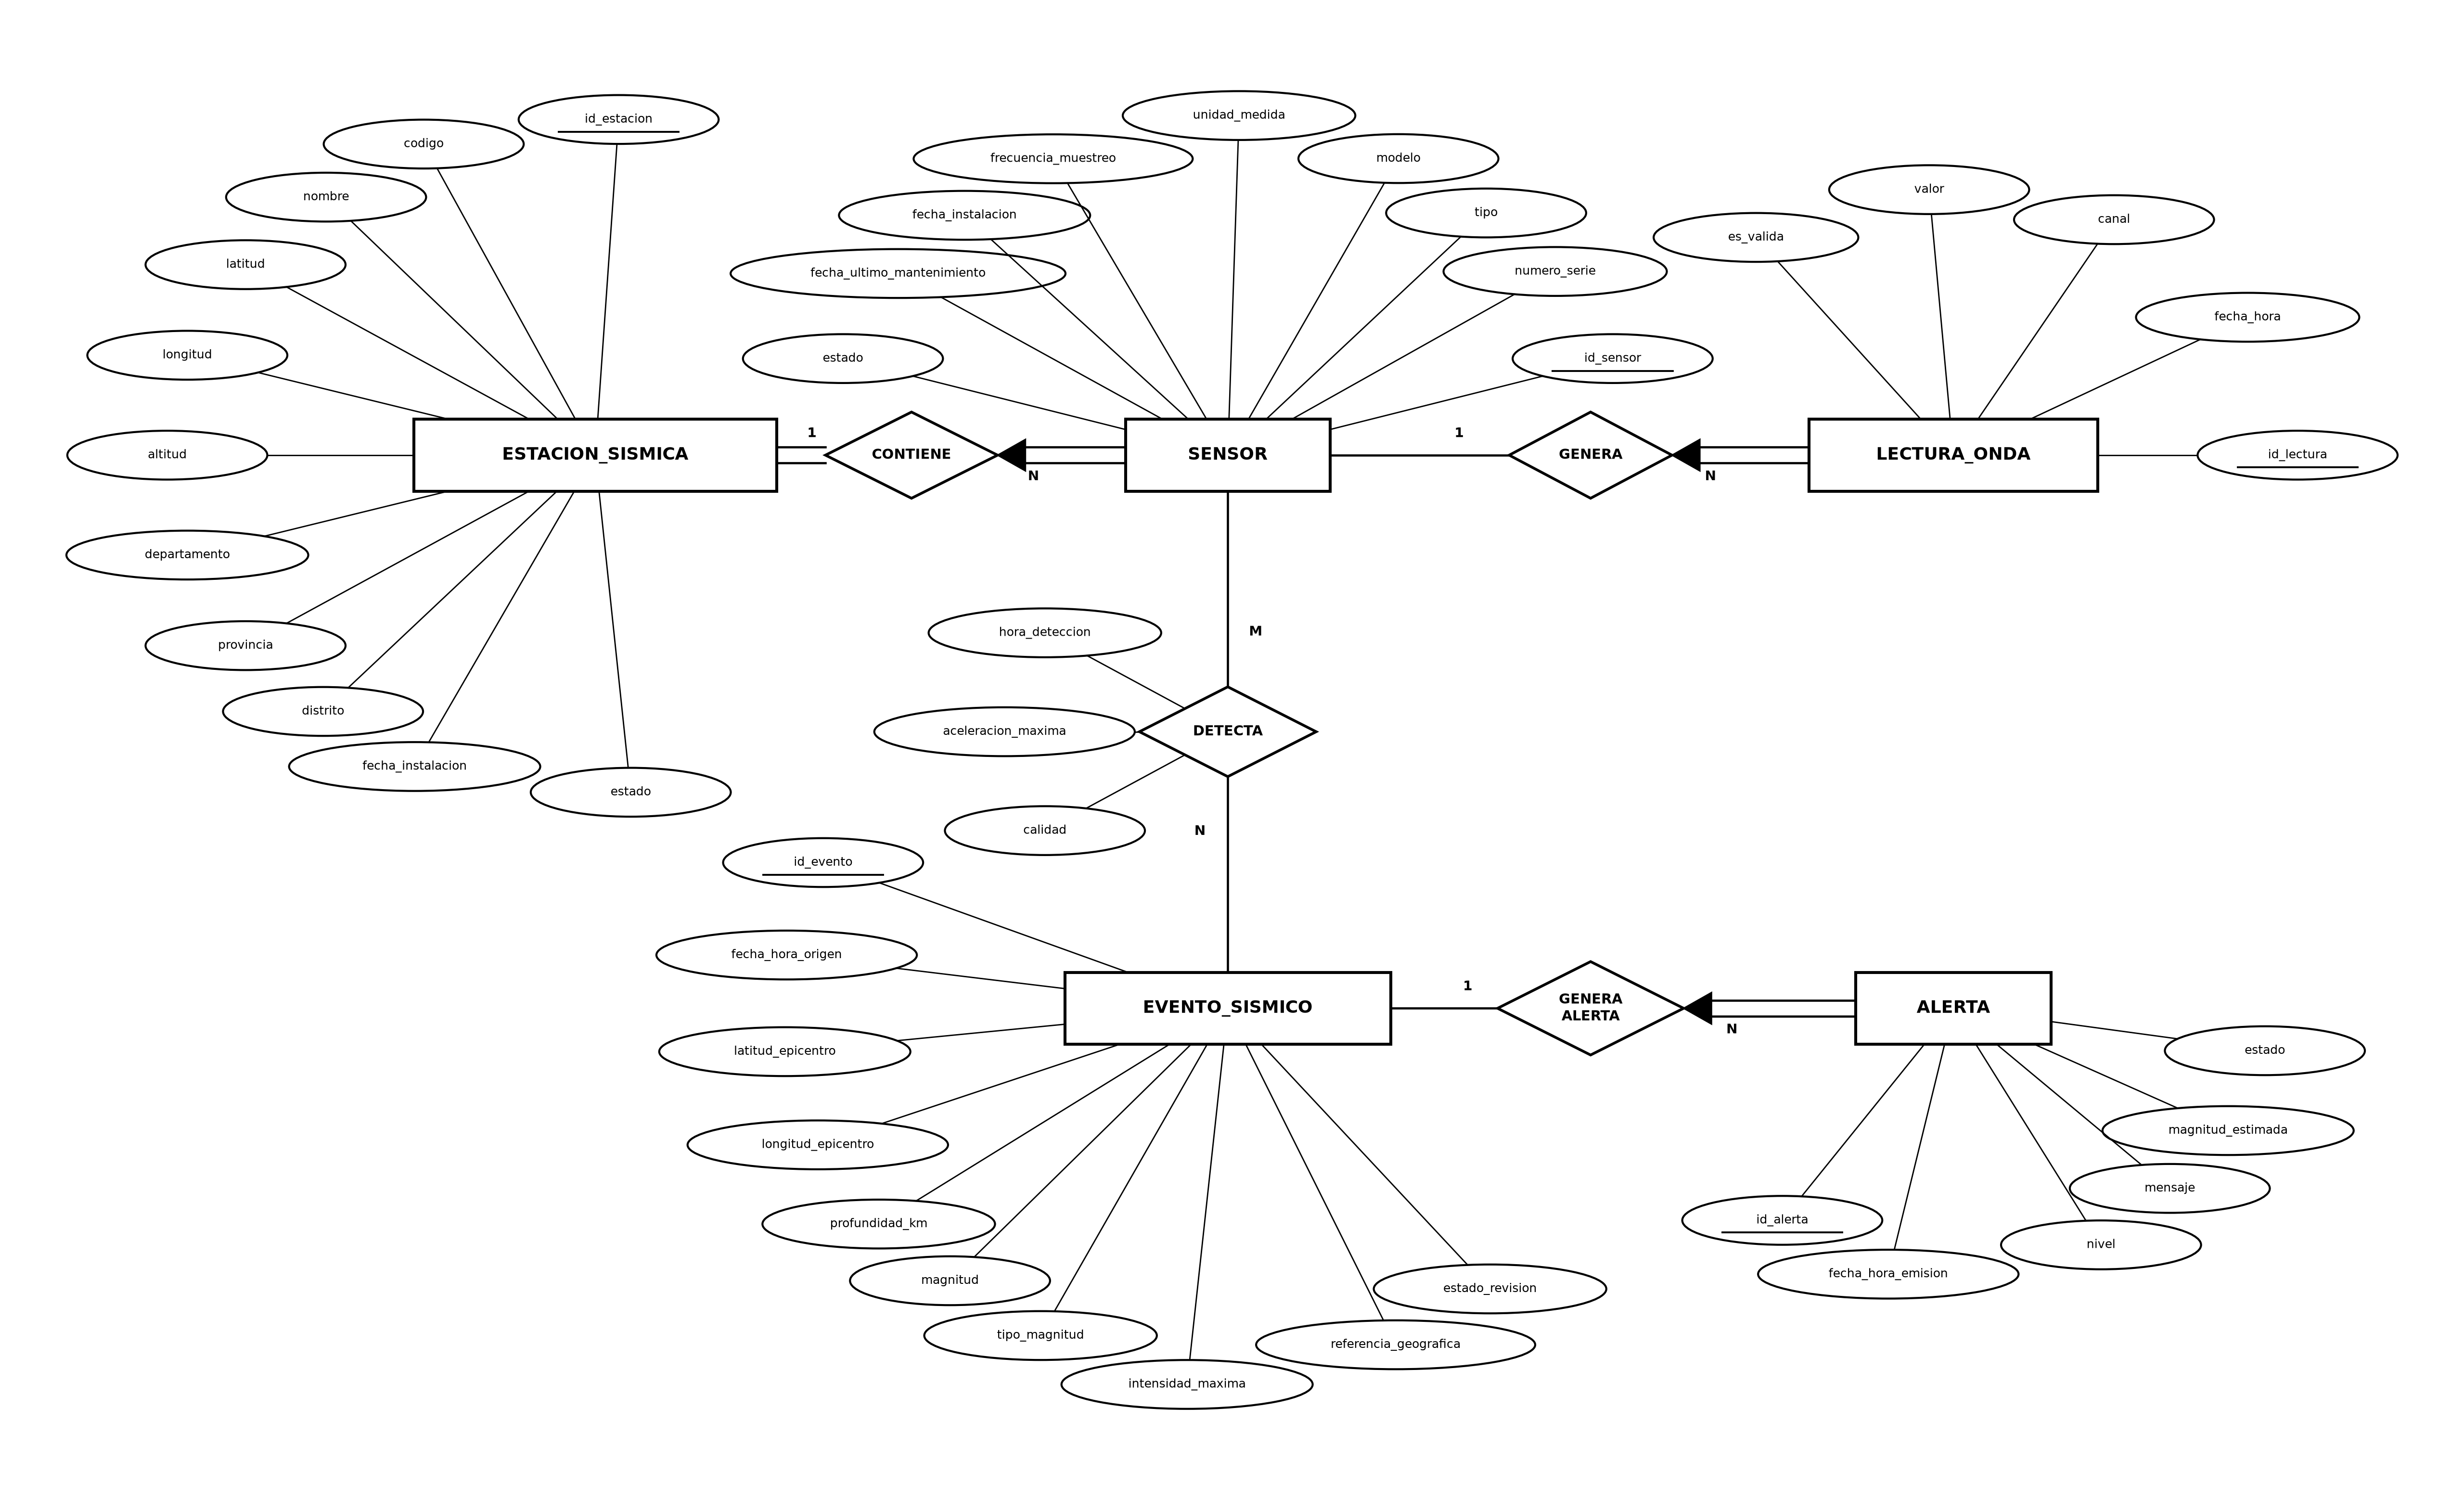
\includegraphics[width=0.98\linewidth,height=0.80\textheight,keepaspectratio]{modelo_er_monitoreo_sismologico_ramakrishnan.png}
    \caption{Modelo Entidad--Relación del sistema de monitoreo sismológico y alerta temprana. Las llaves aparecen subrayadas y se respetan las convenciones de participación y multiplicidad utilizadas en clase.}
    \label{fig:modelo-er}
\end{figure}
\end{landscape}
\clearpage

% -------------------------------------------------
% 2.3
% -------------------------------------------------

\subsection{Especificaciones y consideraciones sobre el modelo}

El modelo Entidad--Relación propuesto representa los principales elementos involucrados en el monitoreo sismológico y en la gestión de alertas tempranas. Se consideran como entidades principales \texttt{ESTACION\_\allowbreak{}SISMICA}, \texttt{SENSOR}, \texttt{LECTURA\_\allowbreak{}ONDA}, \texttt{EVENTO\_\allowbreak{}SISMICO} y \texttt{ALERTA}. Además, se incluye la relación \texttt{DETECTA}, la cual posee atributos propios debido a que representa información específica de la participación de un sensor en la detección de un evento sísmico.

La entidad \texttt{ESTACION\_\allowbreak{}SISMICA} representa cada punto físico de monitoreo y se identifica mediante el atributo llave \texttt{id\_\allowbreak{}estacion}. La relación \texttt{CONTIENE} vincula una estación con los sensores instalados en ella y presenta una multiplicidad uno a muchos. Tanto \texttt{ESTACION\_\allowbreak{}SISMICA} como \texttt{SENSOR} poseen participación total en esta relación, ya que toda estación registrada debe disponer de al menos un sensor y todo sensor debe estar asociado a una única estación. Para el alcance del proyecto, esta asociación representa la instalación actual del sensor y no se conserva el historial de traslados entre estaciones.

La entidad \texttt{SENSOR} se identifica mediante \texttt{id\_\allowbreak{}sensor} y representa los dispositivos encargados de producir las mediciones. Entre sus atributos se incluye \texttt{fecha\_\allowbreak{}ultimo\_\allowbreak{}mantenimiento}, que permite conocer cuándo fue realizada la intervención más reciente sobre el dispositivo. Este atributo puede no tener valor cuando el sensor aún no ha recibido mantenimiento y, cuando exista, su fecha no puede ser anterior a la fecha de instalación. El sistema no mantiene un historial completo de mantenimientos, ya que para el alcance del proyecto se conserva únicamente la última fecha registrada. La relación \texttt{GENERA} vincula \texttt{SENSOR} con \texttt{LECTURA\_\allowbreak{}ONDA} y presenta una multiplicidad uno a muchos. La participación de \texttt{SENSOR} es parcial, ya que un sensor puede existir sin haber generado lecturas, mientras que la participación de \texttt{LECTURA\_\allowbreak{}ONDA} es total debido a que toda lectura debe haber sido producida por un único sensor.

\texttt{LECTURA\_\allowbreak{}ONDA} representa las mediciones individuales obtenidas por los sensores y utiliza \texttt{id\_\allowbreak{}lectura} como atributo llave. Además, incorpora el atributo \texttt{es\_\allowbreak{}valida}, que permite distinguir las mediciones aceptadas para el análisis de aquellas que presentan anomalías o errores instrumentales. Las lecturas no válidas se conservan para mantener la trazabilidad de los datos, pero no se utilizan como sustento de una detección. La entidad se modela de forma independiente debido al elevado volumen de registros que puede generar el monitoreo continuo y a la necesidad de conservar las mediciones para consultas y análisis posteriores.

La entidad \texttt{EVENTO\_\allowbreak{}SISMICO} representa cada sismo registrado dentro del sistema y se identifica mediante \texttt{id\_\allowbreak{}evento}. Sus atributos almacenan información como la fecha y hora de origen, ubicación del epicentro, profundidad, magnitud y otros parámetros descriptivos del evento.

La relación \texttt{DETECTA} conecta \texttt{SENSOR} con \texttt{EVENTO\_\allowbreak{}SISMICO} y posee multiplicidad muchos a muchos. Un sensor puede participar en la detección de múltiples eventos y un mismo evento puede encontrarse asociado a varios sensores. La participación es parcial en ambos lados, ya que un sensor puede no haber participado todavía en ninguna detección y un evento puede existir en la base de datos sin disponer de detecciones instrumentales asociadas.

\texttt{DETECTA} posee los atributos \texttt{hora\_\allowbreak{}deteccion}, \texttt{aceleracion\_\allowbreak{}maxima} y \texttt{calidad}, debido a que estos valores dependen específicamente de la asociación entre un sensor y un evento determinado. En la transformación al modelo relacional, esta relación muchos a muchos dará origen a la relación \texttt{DETECCION}.

La entidad \texttt{ALERTA} representa las alertas registradas a partir de eventos sísmicos y se identifica mediante \texttt{id\_\allowbreak{}alerta}. La relación \texttt{GENERA\_\allowbreak{}ALERTA}, entre \texttt{EVENTO\_\allowbreak{}SISMICO} y \texttt{ALERTA}, presenta multiplicidad uno a muchos. La participación de \texttt{EVENTO\_\allowbreak{}SISMICO} es parcial, debido a que un evento puede no generar ninguna alerta, mientras que la participación de \texttt{ALERTA} es total, ya que toda alerta debe estar asociada obligatoriamente a un único evento.

El atributo \texttt{magnitud\_\allowbreak{}estimada} de \texttt{ALERTA} se mantiene separado de \texttt{magnitud} en \texttt{EVENTO\_\allowbreak{}SISMICO}, ya que representa el valor disponible al momento de emitir la alerta, mientras que la magnitud del evento puede ser revisada o actualizada posteriormente.

En cuanto a la notación utilizada, los atributos llave se encuentran subrayados. Las líneas dobles representan participación total y las líneas simples participación parcial. Las flechas representan restricciones de clave; en las relaciones uno a muchos se dibujan desde la entidad del lado muchos hacia la relación, indicando que cada instancia de dicha entidad puede asociarse, como máximo, con una instancia de la entidad ubicada en el lado uno. Cuando existe simultáneamente participación total y restricción de clave, se mantienen las dos líneas paralelas pero se utiliza una sola punta de flecha. Las relaciones muchos a muchos, como \texttt{DETECTA}, no presentan flechas.

\noindent
\textbf{Matriz de trazabilidad del modelo conceptual.} En la tabla siguiente se vinculan las reglas semánticas con las multiplicidades y participaciones representadas. La expresión \(a..b\) indica el mínimo y máximo de participaciones de una instancia de la entidad en la relación correspondiente.

\begin{longtable}{>{\raggedright\arraybackslash}p{3.0cm} >{\raggedright\arraybackslash}p{8.5cm} >{\raggedright\arraybackslash}p{2.8cm}}
\toprule
\textbf{Relación} & \textbf{Restricción conceptual} & \textbf{Reglas} \\
\midrule
\endfirsthead
\toprule
\textbf{Relación} & \textbf{Restricción conceptual} & \textbf{Reglas} \\
\midrule
\endhead
\texttt{CONTIENE} & Una estación participa en \(1..N\) asociaciones y un sensor en exactamente una. Participación total de ambas entidades; restricción de clave desde \texttt{SENSOR}. & 2--4 \\
\texttt{GENERA} & Un sensor participa en \(0..N\) asociaciones y una lectura en exactamente una. Participación parcial de \texttt{SENSOR} y total de \texttt{LECTURA\_\allowbreak{}ONDA}. & 9--11 \\
\texttt{DETECTA} & Un sensor participa en \(0..N\) detecciones y un evento en \(0..N\). Participación parcial de ambos extremos; sin flechas de restricción de clave. & 15--19 \\
\texttt{GENERA\_\allowbreak{}ALERTA} & Un evento participa en \(0..N\) asociaciones y una alerta en exactamente una. Participación parcial del evento y total de la alerta. & 20--21 \\
\bottomrule
\end{longtable}

\noindent
\textbf{Correspondencia entre entidades, atributos y requerimientos.} La siguiente tabla
complementa la matriz de multiplicidades: muestra cómo los atributos y las
restricciones del modelo responden a las funcionalidades especificadas en la
Sección 1.5.2. La denominación de cada entidad y relación es la misma que se
utiliza en el diagrama y en el modelo relacional.

{\small
\setlength{\tabcolsep}{4pt}
\renewcommand{\arraystretch}{1.15}
\begin{longtable}{>{\raggedright\arraybackslash}p{3.4cm}
                  >{\raggedright\arraybackslash}p{7.0cm}
                  >{\raggedright\arraybackslash}p{3.6cm}}
\toprule
\textbf{Elemento del modelo} & \textbf{Atributos y restricciones relevantes} & \textbf{Requerimientos y reglas} \\
\midrule
\endfirsthead
\toprule
\textbf{Elemento del modelo} & \textbf{Atributos y restricciones relevantes} & \textbf{Requerimientos y reglas} \\
\midrule
\endhead
\texttt{ESTACION\_SISMICA} &
\texttt{id\_estacion} identifica cada estación; \texttt{codigo} es único.
Latitud y longitud tienen los rangos geográficos indicados; la estación
participa totalmente en \texttt{CONTIENE}. &
RF--01; reglas 1--3 y 22. \\
\texttt{SENSOR} &
\texttt{id\_sensor} identifica cada sensor; \texttt{numero\_serie} es
único. La instalación y el mantenimiento siguen un orden temporal;
la relación con su estación es obligatoria. &
RF--02, RF--03; reglas 3--8 y 23--24. \\
\texttt{LECTURA\_ONDA} &
\texttt{id\_lectura} identifica la lectura; sensor, instante y canal
no pueden repetirse como combinación. \texttt{es\_valida} conserva
la distinción entre lecturas aptas y no aptas para análisis. &
RF--04, RF--05; reglas 9--13 y 24. \\
\texttt{EVENTO\_SISMICO} &
\texttt{id\_evento} identifica el evento; el epicentro respeta los
rangos geográficos y la profundidad no puede ser negativa. &
RF--06; reglas 14, 22--23. \\
\texttt{DETECTA} &
La pareja sensor--evento no se repite; hora, aceleración máxima y
calidad dependen de esa asociación. Al transformar esta relación
se obtiene \texttt{DETECCION}. &
RF--07, RF--10; reglas 15--19. \\
\texttt{ALERTA} &
\texttt{id\_alerta} identifica la alerta. Cada alerta pertenece a
un evento; \texttt{magnitud\_estimada} conserva el valor utilizado
en la emisión, independientemente de revisiones posteriores. &
RF--08, RF--09; reglas 20--21 y 25--26. \\
\bottomrule
\end{longtable}
}

\noindent
\textbf{Alcance de las restricciones.} La regla que exige al menos un sensor por estación constituye una participación total del lado de \texttt{ESTACION\_\allowbreak{}SISMICA}, pero no queda garantizada por una llave foránea en \texttt{SENSOR}; su cumplimiento requiere una operación de alta controlada. Por otro lado, el modelo registra la relación entre sensor y evento en \texttt{DETECTA}, pero no registra cuáles lecturas individuales sustentaron esa detección. Por tanto, la regla que exige utilizar lecturas válidas es una condición del proceso de análisis/captura y no puede verificarse retrospectivamente a partir de una llave entre \texttt{DETECCION} y \texttt{LECTURA\_\allowbreak{}ONDA}, pues esa referencia no existe en el modelo actual. Este límite se explicita para no atribuir al diagrama una restricción que no representa.

El modelo no contempla entidades débiles, relaciones ternarias ni jerarquías de generalización o especialización, ya que estas estructuras no son necesarias para representar el alcance definido para el sistema.

% =================================================
% 3. MODELO RELACIONAL
% =================================================

\section{Modelo Relacional}

% -------------------------------------------------
% 3.1
% -------------------------------------------------

\subsection{Modelo Relacional}

A partir del modelo Entidad--Relación definido previamente, se obtiene el siguiente conjunto de relaciones. Para cada atributo se indica su dominio conceptual utilizando los tipos generales trabajados en clase: \texttt{Int}, \texttt{String}, \texttt{Float}, \texttt{Bool} y \texttt{Date}. Los atributos que forman la llave primaria aparecen subrayados. Las llaves foráneas se indican mediante sus referencias y no se subrayan por el solo hecho de ser foráneas. En \texttt{DETECCION}, \texttt{id\_\allowbreak{}sensor} e \texttt{id\_\allowbreak{}evento} aparecen subrayados porque, además de ser llaves foráneas, forman conjuntamente la llave primaria compuesta.

El tipo conceptual \texttt{Date} representa información temporal; los atributos que contienen fecha y hora se implementarán como \texttt{TIMESTAMP} en PostgreSQL, mientras que las fechas sin componente horario se implementarán como \texttt{DATE}. De modo similar, el identificador de lecturas podrá utilizar \texttt{BIGINT} por el volumen previsto. Estas elecciones no modifican las entidades ni sus llaves.


\noindent
\begin{minipage}{\linewidth}
\small\ttfamily\raggedright
ESTACION\_SISMICA(\underline{id\_estacion}:Int, codigo:String,\\
nombre:String, latitud:Float, longitud:Float, altitud:Float,\\
departamento:String, provincia:String, distrito:String,\\
fecha\_instalacion:Date, estado:String)
\end{minipage}
\par\medskip

\begin{itemize}
    \item Llave primaria: \texttt{id\_\allowbreak{}estacion}.
    \item Restricción de unicidad: \texttt{codigo}.
\end{itemize}

\noindent
\begin{minipage}{\linewidth}
\small\ttfamily\raggedright
SENSOR(\underline{id\_sensor}:Int, numero\_serie:String, tipo:String,\\
modelo:String, unidad\_medida:String, frecuencia\_muestreo:Float,\\
fecha\_instalacion:Date, fecha\_ultimo\_mantenimiento:Date,\\
estado:String, id\_estacion:Int)
\end{minipage}
\par\medskip

\begin{itemize}
    \item Llave primaria: \texttt{id\_\allowbreak{}sensor}.
    \item Llave foránea: \texttt{id\_\allowbreak{}estacion} referencia a
    \texttt{ESTACION\_\allowbreak{}SISMICA(id\_\allowbreak{}estacion)}.
    \item Restricción de unicidad: \texttt{numero\_\allowbreak{}serie}.
    \item \texttt{id\_\allowbreak{}estacion} no puede ser nulo, debido a la participación total de \texttt{SENSOR} en la relación \texttt{CONTIENE}.
    \item \texttt{fecha\_\allowbreak{}instalacion} no puede ser nula, porque constituye un dato requerido del sensor según la regla semántica 6.
    \item \texttt{fecha\_\allowbreak{}ultimo\_\allowbreak{}mantenimiento} puede no tener valor si el sensor todavía no ha recibido mantenimiento. Cuando exista, no puede ser anterior a \texttt{fecha\_\allowbreak{}instalacion}.
\end{itemize}

\noindent
\begin{minipage}{\linewidth}
\small\ttfamily\raggedright
LECTURA\_ONDA(\underline{id\_lectura}:Int, id\_sensor:Int,\\
fecha\_hora:Date, canal:String, valor:Float, es\_valida:Bool)
\end{minipage}
\par\medskip

\begin{itemize}
    \item Llave primaria: \texttt{id\_\allowbreak{}lectura}.
    \item Llave foránea: \texttt{id\_\allowbreak{}sensor} referencia a
    \texttt{SENSOR(id\_\allowbreak{}sensor)}.
    \item \texttt{id\_\allowbreak{}sensor} no puede ser nulo, debido a la participación total de \texttt{LECTURA\_\allowbreak{}ONDA} en la relación \texttt{GENERA}.
    \item La combinación \texttt{(id\_\allowbreak{}sensor, fecha\_\allowbreak{}hora, canal)} debe ser única para evitar almacenar dos veces una misma medición del mismo canal e instante.
    \item \texttt{es\_\allowbreak{}valida} indica si la medición puede utilizarse en los análisis y detecciones del sistema.
\end{itemize}

\noindent
\begin{minipage}{\linewidth}
\small\ttfamily\raggedright
EVENTO\_SISMICO(\underline{id\_evento}:Int, fecha\_hora\_origen:Date,\\
latitud\_epicentro:Float, longitud\_epicentro:Float,\\
profundidad\_km:Float, magnitud:Float, tipo\_magnitud:String,\\
intensidad\_maxima:String, referencia\_geografica:String,\\
estado\_revision:String)
\end{minipage}
\par\medskip

\begin{itemize}
    \item Llave primaria: \texttt{id\_\allowbreak{}evento}.
\end{itemize}

\noindent
\begin{minipage}{\linewidth}
\small\ttfamily\raggedright
DETECCION(\underline{id\_sensor}:Int, \underline{id\_evento}:Int,\\
hora\_deteccion:Date, aceleracion\_maxima:Float, calidad:String)
\end{minipage}
\par\medskip

\begin{itemize}
    \item Llave primaria compuesta:
    \texttt{(id\_\allowbreak{}sensor, id\_\allowbreak{}evento)}.
    \item Llave foránea: \texttt{id\_\allowbreak{}sensor} referencia a
    \texttt{SENSOR(id\_\allowbreak{}sensor)}.
    \item Llave foránea: \texttt{id\_\allowbreak{}evento} referencia a
    \texttt{EVENTO\_\allowbreak{}SISMICO(id\_\allowbreak{}evento)}.
\end{itemize}

La relación \texttt{DETECCION} surge de la transformación de la relación muchos a muchos \texttt{DETECTA}. La llave primaria compuesta garantiza, de acuerdo con las reglas semánticas establecidas, que un mismo sensor no registre más de una detección para un mismo evento sísmico.

\noindent
\begin{minipage}{\linewidth}
\small\ttfamily\raggedright
ALERTA(\underline{id\_alerta}:Int, id\_evento:Int,\\
fecha\_hora\_emision:Date, nivel:String, mensaje:String,\\
magnitud\_estimada:Float, estado:String)
\end{minipage}
\par\medskip

\begin{itemize}
    \item Llave primaria: \texttt{id\_\allowbreak{}alerta}.
    \item Llave foránea: \texttt{id\_\allowbreak{}evento} referencia a
    \texttt{EVENTO\_\allowbreak{}SISMICO(id\_\allowbreak{}evento)}.
    \item \texttt{id\_\allowbreak{}evento} no puede ser nulo, debido a la participación total de \texttt{ALERTA} en la relación \texttt{GENERA\_\allowbreak{}ALERTA}.
\end{itemize}

Las relaciones anteriores conservan las dependencias definidas en el modelo Entidad--Relación y evitan almacenar información derivable de otras relaciones. Por ejemplo, la estación asociada a una lectura puede obtenerse a través de \texttt{LECTURA\_\allowbreak{}ONDA}, \texttt{SENSOR} y \texttt{ESTACION\_\allowbreak{}SISMICA}, por lo que no es necesario almacenar \texttt{id\_\allowbreak{}estacion} dentro de cada lectura.

De manera similar, la unidad de medida de una lectura se obtiene a partir del sensor que la generó mediante \texttt{SENSOR.unidad\_\allowbreak{}medida}, evitando repetir este valor en cada registro de \texttt{LECTURA\_\allowbreak{}ONDA}.

La restricción de que toda estación registrada debe poseer al menos un sensor no puede garantizarse únicamente mediante la llave foránea almacenada en \texttt{SENSOR}. Esta condición será considerada durante la implementación mediante mecanismos adicionales de integridad o control de las operaciones de registro.

% -------------------------------------------------
% 3.2
% -------------------------------------------------

\subsection{Especificaciones de transformación}

La transformación del modelo Entidad--Relación al modelo relacional se realizó aplicando las reglas generales de conversión entre ambos modelos. Cada entidad fuerte se convirtió en una relación que conserva sus atributos y utiliza como llave primaria el atributo identificador definido en el modelo conceptual.

Las relaciones uno a muchos se transformaron incorporando la llave primaria de la entidad ubicada en el lado uno como llave foránea en la relación correspondiente al lado muchos. Cuando la participación de esta última es total, dicha llave foránea debe ser obligatoria.

La relación muchos a muchos \texttt{DETECTA}, existente entre \texttt{SENSOR} y \texttt{EVENTO\_\allowbreak{}SISMICO}, se transformó en una nueva relación denominada \texttt{DETECCION}. Esta incorpora las llaves primarias de ambas entidades como llaves foráneas, utiliza su combinación como llave primaria compuesta y conserva los atributos propios de la relación.

La relación uno a muchos entre \texttt{EVENTO\_\allowbreak{}SISMICO} y \texttt{ALERTA} se representó incorporando \texttt{id\_\allowbreak{}evento} como llave foránea dentro de \texttt{ALERTA}.

El modelo no requiere transformaciones asociadas a entidades débiles, relaciones ternarias ni estructuras de generalización o especialización, ya que estos elementos no forman parte del modelo conceptual propuesto.

% -------------------------------------------------
% 3.2.1
% -------------------------------------------------

\subsubsection{Entidades}

Las entidades fuertes del modelo Entidad--Relación se transformaron directamente en relaciones del modelo relacional, conservando sus atributos y utilizando como llave primaria el atributo identificador definido en el modelo conceptual.

De esta manera, \texttt{ESTACION\_\allowbreak{}SISMICA}, \texttt{SENSOR}, \texttt{LECTURA\_\allowbreak{}ONDA}, \texttt{EVENTO\_\allowbreak{}SISMICO} y \texttt{ALERTA} dieron origen a relaciones con el mismo nombre.

En los casos en que una entidad participa en el lado muchos de una relación uno a muchos, la relación resultante incorpora además la llave primaria de la entidad ubicada en el lado uno como llave foránea. Por ello, \texttt{SENSOR} incorpora \texttt{id\_\allowbreak{}estacion}, \texttt{LECTURA\_\allowbreak{}ONDA} incorpora \texttt{id\_\allowbreak{}sensor} y \texttt{ALERTA} incorpora \texttt{id\_\allowbreak{}evento}.

% -------------------------------------------------
% 3.2.2
% -------------------------------------------------

\subsubsection{Entidades débiles}

El modelo Entidad--Relación propuesto no contempla entidades débiles.

Todas las entidades principales poseen un atributo identificador propio que permite distinguir de manera única cada instancia sin depender de la llave de otra entidad para su identificación.

Aunque algunas entidades presentan dependencia de existencia respecto de otras, como \texttt{LECTURA\_\allowbreak{}ONDA} respecto de \texttt{SENSOR} o \texttt{ALERTA} respecto de \texttt{EVENTO\_\allowbreak{}SISMICO}, esta condición no implica que sean entidades débiles. En ambos casos, su identificación se realiza mediante \texttt{id\_\allowbreak{}lectura} e \texttt{id\_\allowbreak{}alerta}, respectivamente.

% -------------------------------------------------
% 3.2.3
% -------------------------------------------------

\subsubsection{Entidades superclase/subclases}

El modelo Entidad--Relación propuesto no contempla estructuras de generalización o especialización mediante superclases y subclases.

Aunque existen distintos tipos de sensores, como acelerómetros o sismómetros, sus diferencias se representan mediante el atributo \texttt{tipo} de \texttt{SENSOR}, ya que para el alcance del proyecto no requieren atributos o relaciones adicionales que justifiquen la creación de subclases independientes.

De manera similar, los distintos niveles o estados de una alerta se representan mediante atributos de \texttt{ALERTA}, sin necesidad de definir una jerarquía de especialización.

% -------------------------------------------------
% 3.2.4
% -------------------------------------------------

\subsubsection{Relaciones binarias}

El modelo Entidad--Relación contiene únicamente relaciones binarias, es decir, relaciones que vinculan dos entidades.

La relación \texttt{CONTIENE}, entre \texttt{ESTACION\_\allowbreak{}SISMICA} y \texttt{SENSOR}, presenta una multiplicidad uno a muchos. Su transformación se realiza incorporando \texttt{id\_\allowbreak{}estacion} como llave foránea en \texttt{SENSOR}. Debido a la participación total de \texttt{SENSOR}, esta referencia es obligatoria.

La relación \texttt{GENERA}, entre \texttt{SENSOR} y \texttt{LECTURA\_\allowbreak{}ONDA}, también presenta una multiplicidad uno a muchos. Por ello, \texttt{id\_\allowbreak{}sensor} se incorpora como llave foránea en \texttt{LECTURA\_\allowbreak{}ONDA}. La participación total de \texttt{LECTURA\_\allowbreak{}ONDA} implica que toda lectura debe estar asociada a un sensor.

La relación \texttt{DETECTA}, entre \texttt{SENSOR} y \texttt{EVENTO\_\allowbreak{}SISMICO}, presenta una multiplicidad muchos a muchos y posee atributos propios. Por esta razón se transforma en la relación \texttt{DETECCION}, que contiene las llaves primarias de ambas entidades como llaves foráneas y utiliza su combinación como llave primaria compuesta.

Finalmente, la relación \texttt{GENERA\_\allowbreak{}ALERTA}, entre \texttt{EVENTO\_\allowbreak{}SISMICO} y \texttt{ALERTA}, presenta una multiplicidad uno a muchos. Su transformación consiste en incorporar \texttt{id\_\allowbreak{}evento} como llave foránea en \texttt{ALERTA}. Debido a la participación total de \texttt{ALERTA}, esta referencia es obligatoria.

% -------------------------------------------------
% 3.2.5
% -------------------------------------------------

\subsubsection{Relaciones ternarias}

El modelo Entidad--Relación propuesto no contempla relaciones ternarias.

Todas las relaciones definidas vinculan únicamente dos entidades. En particular, no es necesario establecer una relación ternaria entre \texttt{ESTACION\_\allowbreak{}SISMICA}, \texttt{SENSOR} y \texttt{EVENTO\_\allowbreak{}SISMICO}, debido a que cada sensor ya se encuentra asociado a una única estación mediante la relación \texttt{CONTIENE}.

Por ello, la estación correspondiente a una detección puede obtenerse a partir del sensor involucrado, sin necesidad de almacenar nuevamente dicha información en la relación \texttt{DETECTA} o en su equivalente relacional \texttt{DETECCION}.

% -------------------------------------------------
% 3.3
% -------------------------------------------------

\subsection{Diccionario de datos}

El diccionario de datos describe los atributos que conforman cada relación del modelo relacional, indicando su tipo de dato, principales restricciones y significado dentro del sistema.

% =================================================
% ESTACION_SISMICA
% =================================================

\subsubsection*{ESTACION\_SISMICA}

{
\small
\setlength{\tabcolsep}{3pt}
\renewcommand{\arraystretch}{1.15}

\begin{longtable}{
    >{\raggedright\arraybackslash}p{4.25cm}
    >{\raggedright\arraybackslash}p{2.65cm}
    >{\raggedright\arraybackslash}p{3.85cm}
    >{\raggedright\arraybackslash}p{3.85cm}
}
\toprule
\textbf{Atributo} &
\textbf{Tipo} &
\textbf{Restricciones} &
\textbf{Descripción} \\
\midrule
\endfirsthead

\toprule
\textbf{Atributo} &
\textbf{Tipo} &
\textbf{Restricciones} &
\textbf{Descripción} \\
\midrule
\endhead

\texttt{id\_\allowbreak{}estacion} &
INTEGER &
PK, NOT NULL &
Identificador único de la estación sísmica. \\

\texttt{codigo} &
VARCHAR &
UNIQUE, NOT NULL &
Código único asignado a la estación. \\

\texttt{nombre} &
VARCHAR &
NOT NULL &
Nombre de la estación sísmica. \\

\texttt{latitud} &
DECIMAL &
NOT NULL, entre $-90$ y $90$ &
Coordenada geográfica de latitud. \\

\texttt{longitud} &
DECIMAL &
NOT NULL, entre $-180$ y $180$ &
Coordenada geográfica de longitud. \\

\texttt{altitud} &
DECIMAL &
--- &
Altitud de la estación respecto al nivel del mar. \\

\texttt{departamento} &
VARCHAR &
--- &
Departamento donde se encuentra ubicada la estación. \\

\texttt{provincia} &
VARCHAR &
--- &
Provincia donde se encuentra ubicada la estación. \\

\texttt{distrito} &
VARCHAR &
--- &
Distrito donde se encuentra ubicada la estación. \\

\texttt{fecha\_\allowbreak{}instalacion} &
DATE &
--- &
Fecha de instalación de la estación. \\

\texttt{estado} &
VARCHAR &
NOT NULL &
Estado operativo actual de la estación. \\

\bottomrule
\end{longtable}
}

% =================================================
% SENSOR
% =================================================

\subsubsection*{SENSOR}

{
\small
\setlength{\tabcolsep}{3pt}
\renewcommand{\arraystretch}{1.15}

\begin{longtable}{
    >{\raggedright\arraybackslash}p{4.25cm}
    >{\raggedright\arraybackslash}p{2.65cm}
    >{\raggedright\arraybackslash}p{3.85cm}
    >{\raggedright\arraybackslash}p{3.85cm}
}
\toprule
\textbf{Atributo} &
\textbf{Tipo} &
\textbf{Restricciones} &
\textbf{Descripción} \\
\midrule
\endfirsthead

\toprule
\textbf{Atributo} &
\textbf{Tipo} &
\textbf{Restricciones} &
\textbf{Descripción} \\
\midrule
\endhead

\texttt{id\_\allowbreak{}sensor} &
INTEGER &
PK, NOT NULL &
Identificador único del sensor. \\

\texttt{numero\_\allowbreak{}serie} &
VARCHAR &
UNIQUE, NOT NULL &
Número de serie único del dispositivo. \\

\texttt{tipo} &
VARCHAR &
NOT NULL &
Tipo de sensor utilizado para el monitoreo. \\

\texttt{modelo} &
VARCHAR &
--- &
Modelo del dispositivo. \\

\texttt{unidad\_\allowbreak{}medida} &
VARCHAR &
NOT NULL &
Unidad utilizada para expresar las mediciones generadas por el sensor. \\

\texttt{frecuencia\_\allowbreak{}muestreo} &
DECIMAL &
NOT NULL, $>0$ &
Frecuencia con la que el sensor genera mediciones. \\

\texttt{fecha\_\allowbreak{}instalacion} &
DATE &
NOT NULL &
Fecha de instalación del sensor en su estación actual. \\

\texttt{fecha\_\allowbreak{}ultimo\_\allowbreak{}mantenimiento} &
DATE &
Puede ser nulo; si existe, no puede ser anterior a \texttt{fecha\_\allowbreak{}instalacion} &
Fecha del mantenimiento más reciente realizado al sensor. \\

\texttt{estado} &
VARCHAR &
NOT NULL &
Estado operativo actual del sensor. \\

\texttt{id\_\allowbreak{}estacion} &
INTEGER &
FK, NOT NULL &
Estación sísmica en la que se encuentra instalado actualmente el sensor. \\

\bottomrule
\end{longtable}
}

\noindent
\texttt{id\_\allowbreak{}estacion}
$\rightarrow$
\texttt{ESTACION\_\allowbreak{}SISMICA(id\_\allowbreak{}estacion)}

% =================================================
% LECTURA_ONDA
% =================================================

\subsubsection*{LECTURA\_ONDA}

{
\small
\setlength{\tabcolsep}{3pt}
\renewcommand{\arraystretch}{1.15}

\begin{longtable}{
    >{\raggedright\arraybackslash}p{4.25cm}
    >{\raggedright\arraybackslash}p{2.65cm}
    >{\raggedright\arraybackslash}p{3.85cm}
    >{\raggedright\arraybackslash}p{3.85cm}
}
\toprule
\textbf{Atributo} &
\textbf{Tipo} &
\textbf{Restricciones} &
\textbf{Descripción} \\
\midrule
\endfirsthead

\toprule
\textbf{Atributo} &
\textbf{Tipo} &
\textbf{Restricciones} &
\textbf{Descripción} \\
\midrule
\endhead

\texttt{id\_\allowbreak{}lectura} &
BIGINT &
PK, NOT NULL &
Identificador único de la lectura. \\

\texttt{id\_\allowbreak{}sensor} &
INTEGER &
FK, NOT NULL &
Sensor que generó la lectura. \\

\texttt{fecha\_\allowbreak{}hora} &
TIMESTAMP &
NOT NULL &
Fecha y hora en la que fue registrada la medición. \\

\texttt{canal} &
VARCHAR &
NOT NULL &
Canal o componente de medición correspondiente a la lectura. \\

\texttt{valor} &
DECIMAL &
NOT NULL &
Valor numérico registrado por el sensor. \\

\texttt{es\_\allowbreak{}valida} &
BOOLEAN &
NOT NULL &
Indica si la lectura puede utilizarse en los análisis y detecciones del sistema. \\

\bottomrule
\end{longtable}
}

\noindent
\texttt{id\_\allowbreak{}sensor}
$\rightarrow$
\texttt{SENSOR(id\_\allowbreak{}sensor)}

La combinación \texttt{(id\_\allowbreak{}sensor, fecha\_\allowbreak{}hora, canal)} debe ser única para evitar el registro duplicado de una misma medición. Se utiliza \texttt{BIGINT} para \texttt{id\_\allowbreak{}lectura} debido al elevado volumen de registros que esta relación puede alcanzar.

La unidad correspondiente a una lectura se obtiene mediante el atributo \texttt{unidad\_\allowbreak{}medida} del sensor que la generó, por lo que no se almacena nuevamente en \texttt{LECTURA\_\allowbreak{}ONDA}.

% =================================================
% EVENTO_SISMICO
% =================================================

\subsubsection*{EVENTO\_SISMICO}

{
\small
\setlength{\tabcolsep}{3pt}
\renewcommand{\arraystretch}{1.15}

\begin{longtable}{
    >{\raggedright\arraybackslash}p{4.25cm}
    >{\raggedright\arraybackslash}p{2.65cm}
    >{\raggedright\arraybackslash}p{3.85cm}
    >{\raggedright\arraybackslash}p{3.85cm}
}
\toprule
\textbf{Atributo} &
\textbf{Tipo} &
\textbf{Restricciones} &
\textbf{Descripción} \\
\midrule
\endfirsthead

\toprule
\textbf{Atributo} &
\textbf{Tipo} &
\textbf{Restricciones} &
\textbf{Descripción} \\
\midrule
\endhead

\texttt{id\_\allowbreak{}evento} &
INTEGER &
PK, NOT NULL &
Identificador único del evento sísmico. \\

\texttt{fecha\_\allowbreak{}hora\_\allowbreak{}origen} &
TIMESTAMP &
NOT NULL &
Fecha y hora estimada de origen del evento. \\

\texttt{latitud\_\allowbreak{}epicentro} &
DECIMAL &
NOT NULL, entre $-90$ y $90$ &
Latitud estimada del epicentro. \\

\texttt{longitud\_\allowbreak{}epicentro} &
DECIMAL &
NOT NULL, entre $-180$ y $180$ &
Longitud estimada del epicentro. \\

\texttt{profundidad\_\allowbreak{}km} &
DECIMAL &
NOT NULL, $\geq 0$ &
Profundidad estimada del evento en kilómetros. \\

\texttt{magnitud} &
DECIMAL &
NOT NULL &
Magnitud registrada para el evento. \\

\texttt{tipo\_\allowbreak{}magnitud} &
VARCHAR &
--- &
Tipo o escala utilizada para expresar la magnitud. \\

\texttt{intensidad\_\allowbreak{}maxima} &
VARCHAR &
--- &
Intensidad máxima reportada para el evento. \\

\texttt{referencia\_\allowbreak{}geografica} &
VARCHAR &
--- &
Descripción geográfica aproximada de la ubicación del evento. \\

\texttt{estado\_\allowbreak{}revision} &
VARCHAR &
NOT NULL &
Estado de revisión de la información del evento. \\

\bottomrule
\end{longtable}
}

% =================================================
% DETECCION
% =================================================

\subsubsection*{DETECCION}

{
\small
\setlength{\tabcolsep}{3pt}
\renewcommand{\arraystretch}{1.15}

\begin{longtable}{
    >{\raggedright\arraybackslash}p{4.25cm}
    >{\raggedright\arraybackslash}p{2.65cm}
    >{\raggedright\arraybackslash}p{3.85cm}
    >{\raggedright\arraybackslash}p{3.85cm}
}
\toprule
\textbf{Atributo} &
\textbf{Tipo} &
\textbf{Restricciones} &
\textbf{Descripción} \\
\midrule
\endfirsthead

\toprule
\textbf{Atributo} &
\textbf{Tipo} &
\textbf{Restricciones} &
\textbf{Descripción} \\
\midrule
\endhead

\texttt{id\_\allowbreak{}sensor} &
INTEGER &
PK, FK, NOT NULL &
Sensor que participó en la detección. \\

\texttt{id\_\allowbreak{}evento} &
INTEGER &
PK, FK, NOT NULL &
Evento sísmico asociado a la detección. \\

\texttt{hora\_\allowbreak{}deteccion} &
TIMESTAMP &
NOT NULL &
Momento en que el sensor registró la detección del evento. \\

\texttt{aceleracion\_\allowbreak{}maxima} &
DECIMAL &
Si existe, $\geq 0$ &
Magnitud máxima de aceleración registrada durante la detección. \\

\texttt{calidad} &
VARCHAR &
--- &
Indicador de calidad asociado a la detección. \\

\bottomrule
\end{longtable}
}

La llave primaria es compuesta:

\noindent
\texttt{PK(id\_\allowbreak{}sensor, id\_\allowbreak{}evento)}

Las referencias son:

\noindent
\texttt{id\_\allowbreak{}sensor}
$\rightarrow$
\texttt{SENSOR(id\_\allowbreak{}sensor)}

\noindent
\texttt{id\_\allowbreak{}evento}
$\rightarrow$
\texttt{EVENTO\_\allowbreak{}SISMICO(id\_\allowbreak{}evento)}

La llave compuesta garantiza que un mismo sensor registre como máximo una detección asociada a un mismo evento sísmico dentro del modelo planteado.

% =================================================
% ALERTA
% =================================================

\subsubsection*{ALERTA}

{
\small
\setlength{\tabcolsep}{3pt}
\renewcommand{\arraystretch}{1.15}

\begin{longtable}{
    >{\raggedright\arraybackslash}p{4.25cm}
    >{\raggedright\arraybackslash}p{2.65cm}
    >{\raggedright\arraybackslash}p{3.85cm}
    >{\raggedright\arraybackslash}p{3.85cm}
}
\toprule
\textbf{Atributo} &
\textbf{Tipo} &
\textbf{Restricciones} &
\textbf{Descripción} \\
\midrule
\endfirsthead

\toprule
\textbf{Atributo} &
\textbf{Tipo} &
\textbf{Restricciones} &
\textbf{Descripción} \\
\midrule
\endhead

\texttt{id\_\allowbreak{}alerta} &
INTEGER &
PK, NOT NULL &
Identificador único de la alerta. \\

\texttt{id\_\allowbreak{}evento} &
INTEGER &
FK, NOT NULL &
Evento sísmico asociado a la alerta. \\

\texttt{fecha\_\allowbreak{}hora\_\allowbreak{}emision} &
TIMESTAMP &
NOT NULL &
Fecha y hora de emisión de la alerta. \\

\texttt{nivel} &
VARCHAR &
NOT NULL &
Nivel asignado a la alerta. \\

\texttt{mensaje} &
VARCHAR &
NOT NULL &
Contenido informativo de la alerta. \\

\texttt{magnitud\_\allowbreak{}estimada} &
DECIMAL &
Puede ser nulo &
Magnitud estimada disponible al momento de emitir la alerta. \\

\texttt{estado} &
VARCHAR &
NOT NULL &
Estado actual de la alerta. \\

\bottomrule
\end{longtable}
}

\noindent
\texttt{id\_\allowbreak{}evento}
$\rightarrow$
\texttt{EVENTO\_\allowbreak{}SISMICO(id\_\allowbreak{}evento)}

La magnitud sísmica y la magnitud estimada no tienen en este diseño una restricción general de no negatividad: las escalas de magnitud pueden expresar valores negativos. En cambio, la profundidad y la aceleración máxima expresada como magnitud no pueden ser negativas. Los valores permitidos para los estados categóricos se precisarán en la implementación sin contradecir las reglas de operación del sensor.

Las restricciones descritas en este diccionario establecen los principales dominios y condiciones de integridad del modelo relacional. Durante la implementación en PostgreSQL se materializarán mediante tipos de datos específicos, restricciones \texttt{PRIMARY KEY}, \texttt{FOREIGN KEY}, \texttt{UNIQUE}, \texttt{NOT NULL} y \texttt{CHECK}, según corresponda.

% =================================================
% 4. IMPLEMENTACION DE LA BASE DE DATOS
% =================================================
\clearpage
\section{Implementación de la base de datos}

\subsection{Creación de Tablas en PostgreSQL}

La estructura física del sistema se implementó en PostgreSQL 18.6, dentro
 del esquema \texttt{monitoreo\_sismologico}. Se conservaron las seis
 relaciones del modelo relacional de la Sección 3.1 y se definieron sus
 claves, restricciones de dominio y referencias entre tablas. La relación
 \texttt{DETECCION} mantiene la clave primaria compuesta
 \texttt{(id\_sensor, id\_evento)}, correspondiente a la relación
 muchos a muchos del modelo conceptual.

Los identificadores emplean \texttt{INTEGER}, con excepción de
 \texttt{id\_lectura}, definido como \texttt{BIGINT} por el volumen de
 mediciones. Las claves simples utilizan \texttt{GENERATED BY DEFAULT AS
 IDENTITY}; los instantes se almacenan mediante \texttt{TIMESTAMP}, y
 los atributos cuantitativos mediante \texttt{NUMERIC}. La creación
 de las seis tablas precede a la incorporación de restricciones con
 \texttt{ALTER TABLE}.

\begin{table}[H]
\centering
\small
\begin{tabular}{@{}>{\raggedright\arraybackslash}p{0.22\linewidth}>{\raggedright\arraybackslash}p{0.25\linewidth}>{\raggedright\arraybackslash}p{0.43\linewidth}@{}}
\toprule
\textbf{Relación} & \textbf{Clave primaria} & \textbf{Integridad principal} \\
\midrule
\texttt{estacion\_sismica} & \texttt{id\_estacion} & Código único y coordenadas válidas. \\
\texttt{sensor} & \texttt{id\_sensor} & Referencia a estación, serie única y frecuencia positiva. \\
\texttt{lectura\_onda} & \texttt{id\_lectura} & Referencia al sensor y combinación sensor--fecha--canal única. \\
\texttt{evento\_sismico} & \texttt{id\_evento} & Rango de coordenadas y profundidad no negativa. \\
\texttt{deteccion} & \texttt{(id\_sensor, id\_evento)} & Referencias a sensor y evento; aceleración no negativa si se registra. \\
\texttt{alerta} & \texttt{id\_alerta} & Referencia al evento sísmico. \\
\bottomrule
\end{tabular}
\caption{Claves y principales restricciones implementadas en PostgreSQL.}
\label{tab:estructura-resumen-41}
\end{table}

\subsubsection*{Definición de tablas y restricciones}

El siguiente fragmento muestra la definición de una estación y el uso
 de \texttt{ALTER TABLE} para incorporar las restricciones que verifican
 sus coordenadas y la unicidad del código.

\begin{sqlbloque}{Estructura y restricciones de estación (01\_estructura.sql)}
CREATE TABLE estacion_sismica (
    id_estacion INTEGER GENERATED BY DEFAULT AS IDENTITY,
    codigo VARCHAR(50) NOT NULL,
    nombre VARCHAR(150) NOT NULL,
    latitud NUMERIC NOT NULL,
    longitud NUMERIC NOT NULL,
    altitud NUMERIC,
    departamento VARCHAR(100),
    provincia VARCHAR(100),
    distrito VARCHAR(100),
    fecha_instalacion DATE,
    estado VARCHAR(40) NOT NULL
);

ALTER TABLE estacion_sismica
    ADD CONSTRAINT pk_estacion_sismica PRIMARY KEY (id_estacion);
ALTER TABLE estacion_sismica
    ADD CONSTRAINT uq_estacion_codigo UNIQUE (codigo);
ALTER TABLE estacion_sismica
    ADD CONSTRAINT ck_estacion_latitud CHECK (latitud BETWEEN -90 AND 90),
    ADD CONSTRAINT ck_estacion_longitud CHECK (longitud BETWEEN -180 AND 180);
\end{sqlbloque}

En \texttt{DETECCION} se implementaron dos claves foráneas y una clave
 primaria compuesta, de modo que no se puede repetir la asociación
 entre el mismo sensor y evento sísmico.

\begin{sqlbloque}{Clave compuesta y referencias de detección (01\_estructura.sql)}
CREATE TABLE deteccion (
    id_sensor INTEGER NOT NULL,
    id_evento INTEGER NOT NULL,
    hora_deteccion TIMESTAMP NOT NULL,
    aceleracion_maxima NUMERIC,
    calidad VARCHAR(40)
);

ALTER TABLE deteccion
    ADD CONSTRAINT pk_deteccion PRIMARY KEY (id_sensor, id_evento);
ALTER TABLE deteccion
    ADD CONSTRAINT fk_deteccion_sensor
    FOREIGN KEY (id_sensor) REFERENCES sensor(id_sensor),
    ADD CONSTRAINT fk_deteccion_evento
    FOREIGN KEY (id_evento) REFERENCES evento_sismico(id_evento);
ALTER TABLE deteccion
    ADD CONSTRAINT ck_deteccion_aceleracion
    CHECK (aceleracion_maxima IS NULL OR aceleracion_maxima >= 0);
\end{sqlbloque}

Las definiciones restantes, con sus atributos y restricciones completas,
 se encuentran en el integrador \texttt{sql/01\_estructura.sql} del
 repositorio del proyecto.

\subsubsection*{Verificación de la estructura y la integridad}

La comprobación registrada con PostgreSQL identificó seis tablas y
 seis claves primarias, cinco foráneas, tres restricciones de unicidad
 y ocho de tipo \texttt{CHECK}. El catálogo registró además 36
 restricciones de obligatoriedad asociadas a \texttt{NOT NULL}.
 El integrador incorporó pruebas de inserción para comprobar tanto
 la aceptación de registros válidos como el rechazo de operaciones
 que vulneraban las restricciones.

\begin{table}[H]
\centering
\small
\begin{tabular}{@{}p{0.68\linewidth}p{0.23\linewidth}@{}}
\toprule
\textbf{Prueba de integridad} & \textbf{Resultado} \\
\midrule
Latitud de estación fuera del intervalo permitido & Rechazada \\
Frecuencia de muestreo igual a cero & Rechazada \\
Duplicación de sensor, instante y canal de lectura & Rechazada \\
Alerta referida a un evento inexistente & Rechazada \\
Duplicación del par sensor--evento en detección & Rechazada \\
\bottomrule
\end{tabular}
\caption{Rechazos de integridad comprobados durante la validación de la estructura.}
\label{tab:estructura-pruebas-41}
\end{table}

Estas inserciones se realizaron en una transacción de comprobación
 finalizada con \texttt{ROLLBACK}, por lo que los datos de prueba
 no permanecieron almacenados.

\subsubsection*{Alcance de las restricciones}

Las claves foráneas impiden, por ejemplo, registrar un sensor sin
 estación, pero no garantizan que toda estación cuente con al menos
 un sensor. Esta última regla requiere un mecanismo adicional de
 registro o validación. Asimismo, impedir nuevas lecturas válidas
 de sensores inoperativos depende del estado de otra relación y
 se aborda como regla de negocio en la Sección 4.6, no mediante
 una restricción \texttt{CHECK} sobre \texttt{LECTURA\_ONDA}.
 El modelo tampoco registra una referencia directa de cada detección
 hacia las lecturas individuales que la sustentan.

Para la experimentación del Capítulo 5 se diferencian los índices
 necesarios para \texttt{PRIMARY KEY} y \texttt{UNIQUE} de los
 índices secundarios candidatos a optimizar las consultas.


% =================================================
% 4.2 CARGA DE DATOS: LOTE SINTETICO Y CATALOGO IGP
% =================================================

\subsection{Carga de datos}\label{sec:carga-datos-42}

La carga de datos se realizó mediante el integrador
\texttt{sql/02\_datos.sql}, ejecutado con \texttt{psql} sobre las seis
relaciones creadas en PostgreSQL. El procedimiento verifica previamente
que las tablas estén vacías y efectúa, dentro de una misma transacción,
la carga inicial, la importación del catálogo sísmico del Instituto
Geofísico del Perú (IGP) y la simulación complementaria descrita en
la Sección~\ref{sec:simulacion-43}. La confirmación mediante
\texttt{COMMIT} ocurre al finalizar las tres etapas y sus comprobaciones.

\subsubsection*{Carga inicial de datos sintéticos}

La primera etapa incorporó registros definidos en el integrador mediante
\texttt{INSERT INTO}, respetando las dependencias entre estaciones,
sensores, lecturas, eventos, detecciones y alertas. Esta carga proporciona
casos de prueba de las relaciones y restricciones, sin representar
operaciones de una red sísmica real.

\begin{table}[H]
\centering
\begin{tabular}{lrr}
\toprule
\textbf{Relación} & \textbf{Esperados} & \textbf{Verificados} \\
\midrule
\texttt{ESTACION\_SISMICA} & 5 & 5 \\
\texttt{SENSOR} & 10 & 10 \\
\texttt{LECTURA\_ONDA} & 190 & 190 \\
\texttt{EVENTO\_SISMICO} & 8 & 8 \\
\texttt{DETECCION} & 14 & 14 \\
\texttt{ALERTA} & 5 & 5 \\
\midrule
\textbf{Total} & \textbf{232} & \textbf{232} \\
\bottomrule
\end{tabular}
\caption{Recuentos verificados de la carga sintética inicial.}
\label{tab:carga-inicial-42}
\end{table}

De las 190 lecturas insertadas, 166 se registraron como válidas y 24
como inválidas. Los controles del integrador no detectaron estaciones
sin sensores, lecturas huérfanas, detecciones sin lectura válida
asociada ni lecturas válidas provenientes de sensores no operativos.
Estos resultados corresponden al conjunto cargado y no sustituyen las
restricciones permanentes descritas en las Secciones 4.1, 4.5 y 4.6.

\subsubsection*{Importación del catálogo sísmico del IGP}

La fuente externa es el recurso \emph{Dataset del Catálogo Sísmico desde
1960 al 2025}, publicado por el IGP en la Plataforma Nacional de Datos
Abiertos\footnote{Recurso utilizado:
\url{https://www.datosabiertos.gob.pe/dataset/catalogo-sismico/resource/f9629081-0721-4101-a2c2-d0622e046f8b}.}.
El archivo contiene 24\,289 eventos en ocho columnas, con separador
punto y coma. Para reproducir la importación, el CSV de ese recurso se
ubica como \texttt{sql/datos/igp\_catalogo.csv}, según las instrucciones
de preparación del repositorio.

El integrador emplea \texttt{\textbackslash copy} de \texttt{psql}
para cargar las ocho columnas como texto en una tabla temporal,
\texttt{igp\_catalogo\_42}. Antes de su inserción se comprueban los
campos obligatorios, los identificadores repetidos, los formatos de
fecha y hora y los rangos de coordenadas y profundidad. La tabla
intermedia se elimina al confirmar la transacción mediante
\texttt{ON COMMIT DROP}.

\begin{sqlbloque}{Carga del catálogo IGP (02\_datos.sql)}
\copy igp_catalogo_42 (id, fecha_utc, hora_utc, latitud, longitud, profundidad, magnitud, fecha_corte) FROM 'datos/igp_catalogo.csv' WITH (FORMAT csv, HEADER true, DELIMITER ';', ENCODING 'UTF8')
\end{sqlbloque}

Los campos \texttt{FECHA\_UTC} y \texttt{HORA\_UTC} se combinan en
\texttt{fecha\_hora\_origen}; las horas se completan a seis dígitos
para preservar los ceros iniciales. La columna se define como
\texttt{TIMESTAMP} sin zona horaria, por lo que se conserva la
interpretación UTC de la fuente. Las coordenadas, la profundidad y la
magnitud se convierten a tipos numéricos.

El identificador interno se construye como \texttt{200000000 + ID} del
catálogo, separándolo de los ocho eventos sintéticos originales. Los
campos no disponibles en el CSV (\texttt{tipo\_magnitud},
\texttt{intensidad\_maxima} y \texttt{referencia\_geografica})
permanecen en \texttt{NULL}. El valor \texttt{pendiente\_revision}
es un estado administrativo del sistema y no un atributo proporcionado
por el IGP.

\begin{table}[H]
\centering
\begin{tabular}{p{9.8cm}r}
\toprule
\textbf{Comprobación} & \textbf{Resultado} \\
\midrule
Filas del CSV incorporadas a la tabla temporal & 24\,289 \\
Eventos del IGP insertados en \texttt{EVENTO\_SISMICO} & 24\,289 \\
Eventos sintéticos de la etapa inicial conservados & 8 \\
Eventos acumulados antes de la simulación complementaria & 24\,297 \\
Eventos importados con coordenadas o profundidad fuera de rango & 0 \\
Eventos con atributos ausentes rellenados artificialmente & 0 \\
\bottomrule
\end{tabular}
\caption{Controles de la importación del catálogo sísmico del IGP.}
\label{tab:igp-importacion-42}
\end{table}

La salida de la ejecución registró \texttt{COPY 24289} y
\texttt{INSERT 0 24289}. En el conjunto importado, el primer evento
corresponde al 13 de enero de 1960 a las 15:40:34 UTC y el último al
31 de diciembre de 2025 a las 20:34:41 UTC; las magnitudes registradas
van de 3 a 8,4. Estos valores describen la versión del catálogo
empleada en las pruebas.

\subsubsection*{Estado de la carga antes de la simulación complementaria}

Al finalizar estas dos etapas, los controles internos de la transacción
registraron \textbf{24\,521 filas}: 232 del lote sintético inicial y
24\,289 eventos del IGP. Ninguna detección ni alerta sintética fue
asociada a los eventos oficiales durante esta importación. La cifra
corresponde a un estado intermedio de la ejecución; la transacción se
confirma después de la simulación complementaria de la
Sección~\ref{sec:simulacion-43}.

\subsection{Simulación de datos faltantes}\label{sec:simulacion-43}

\subsubsection*{Procedencia y propósito de la simulación}

El catálogo del Instituto Geofísico del Perú (IGP) aporta información
sobre los eventos sísmicos, pero no incluye las estaciones, los sensores,
las lecturas instrumentales, las detecciones ni las alertas requeridas
para evaluar las operaciones del sistema. Por ello, se incorporó un lote
\textbf{sintético y reproducible} que complementa los registros de la
Sección~\ref{sec:carga-datos-42}.

Las estaciones simuladas se identifican mediante códigos
\texttt{SIM43-EST-}, los sensores mediante \texttt{SIM43-SEN-} y
los demás registros mediante rangos de identificadores reservados.
Los 24\,289 eventos importados del IGP permanecen diferenciados:
no se les asocian detecciones ni alertas ficticias, ni se completan
arbitrariamente atributos no publicados por la fuente.

\subsubsection*{Generación de los datos}

La tercera etapa del integrador \nolinkurl{sql/02_datos.sql} emplea
\texttt{generate\_series} y expresiones deterministas de PostgreSQL.
No requiere bibliotecas externas ni valores aleatorios. El siguiente
fragmento ilustra la generación de las diez estaciones adicionales:

\begin{sqlbloque}{Estaciones simuladas mediante generate\_series (02\_datos.sql)}
INSERT INTO estacion_sismica (
    id_estacion, codigo, nombre, latitud, longitud, altitud,
    departamento, provincia, distrito, fecha_instalacion, estado
)
SELECT
    820300001 + g,
    'SIM43-EST-' || LPAD((g + 1)::TEXT, 2, '0'),
    'Estacion simulada de prueba ' || LPAD((g + 1)::TEXT, 2, '0'),
    -5.5::NUMERIC - g * 1.1::NUMERIC,
    -78.4::NUMERIC + g * 0.21::NUMERIC,
    100::NUMERIC + g * 85::NUMERIC,
    NULL, NULL, NULL, DATE '2024-01-01', 'operativa'
FROM generate_series(0, 9) AS serie(g);
\end{sqlbloque}

Cada estación adicional recibe tres sensores operativos. Las 1\,000
lecturas se generan para esos treinta sensores, con fechas y canales
calculados de forma determinista; 947 se marcan como válidas y 53 como
inválidas. Los valores de la señal pueden ser negativos, porque
representan mediciones con signo. Por separado, se generan treinta
eventos sintéticos, noventa detecciones (tres por evento) y
veinticuatro alertas. Las detecciones corresponden a lecturas válidas
del sensor en el mismo instante, y las alertas se emiten después del
origen de los eventos. Se conservan eventos sin alerta, de acuerdo con
la participación opcional prevista en el modelo.

\begin{table}[H]
\centering\small
\begin{tabular}{p{5.3cm}rrr}
\toprule
\textbf{Relación} & \textbf{Antes} & \textbf{Añadidos} & \textbf{Después} \\
\midrule
\texttt{ESTACION\_SISMICA} & 5 & 10 & 15 \\
\texttt{SENSOR} & 10 & 30 & 40 \\
\texttt{LECTURA\_ONDA} & 190 & 1\,000 & 1\,190 \\
\texttt{EVENTO\_SISMICO} & 24\,297 & 30 & 24\,327 \\
\texttt{DETECCION} & 14 & 90 & 104 \\
\texttt{ALERTA} & 5 & 24 & 29 \\
\midrule
\textbf{Total} & \textbf{24\,521} & \textbf{1\,184} & \textbf{25\,705} \\
\bottomrule
\end{tabular}
\caption{Balance de registros antes y después de la simulación complementaria.}
\label{tab:volumen-simulado-43}
\end{table}

\subsubsection*{Controles de integridad y confirmación}

Antes de insertar los datos, el integrador comprueba las cantidades de
la carga inicial y del catálogo IGP, además de verificar que los
identificadores reservados estén libres. Las tres etapas de carga
pertenecen a una \textbf{única transacción}, que se confirma al final
de \texttt{02\_datos.sql} después de las validaciones. Ante un error
que impida confirmar esa transacción, los cambios no confirmados
pueden revertirse.

El integrador comprueba los 1\,184 registros nuevos, la conservación
de los 24\,289 eventos oficiales y el total final de 25\,705 filas.
Los controles de consistencia del lote complementario registraron:

\begin{table}[H]
\centering\small
\begin{tabular}{p{10cm}r}
\toprule
\textbf{Control} & \textbf{Incidencias} \\
\midrule
Estaciones simuladas sin sensor & 0 \\
Lecturas simuladas sin sensor & 0 \\
Lecturas válidas de sensores no operativos & 0 \\
Detecciones sin lectura válida correspondiente & 0 \\
Alertas anteriores a su evento & 0 \\
\bottomrule
\end{tabular}
\caption{Controles de integridad aplicados al lote sintético complementario.}
\label{tab:integridad-simulada-43}
\end{table}

Las fechas de las nuevas lecturas abarcan desde
\texttt{2026-08-01 00:00:00} hasta \texttt{2026-08-30 00:00:29}.
La composición final de la base se verifica mediante:
\[
N_{\mathrm{final}} = N_{\mathrm{inicial}} + N_{\mathrm{IGP}} + N_{\mathrm{complementario}}
= 232 + 24\,289 + 1\,184 = 25\,705.
\]

Estos controles respaldan la coherencia del \emph{conjunto generado},
pero no establecen por sí solos todas las reglas de negocio como
restricciones permanentes. En particular, la relación entre una
detección y una lectura válida se verifica por sensor e instante,
sin una clave foránea directa hacia \texttt{LECTURA\_ONDA}.
Los mecanismos operativos adicionales se presentan en las
Secciones 4.5 y 4.6. La simulación de este apartado es diferente de
las bases experimentales utilizadas para medir rendimiento en el
Capítulo~5.


% =================================================
% 4.4. VISTAS
% =================================================

\subsection{Vistas (Views)}
\label{sec:vistas-proyecto}

\subsubsection*{Diseño y finalidad}

Se implementaron cinco vistas sobre las seis relaciones base mediante
\texttt{CREATE OR REPLACE VIEW}. Su finalidad es facilitar la recuperación
de información de estaciones, sensores, eventos y alertas, así como
la elaboración de resúmenes del catálogo sísmico del Instituto Geofísico
del Perú (IGP). Las vistas son convencionales: sus resultados se calculan
al consultarlas y no requieren almacenar nuevas copias de los registros.

\begin{table}[H]
\centering\small
\begin{tabular}{>{\raggedright\arraybackslash}p{5.2cm}>{\raggedright\arraybackslash}p{8.7cm}}
\toprule
\textbf{Vista} & \textbf{Información proporcionada} \\
\midrule
\texttt{vw\_sensores\_actividad} & Actividad, estado y lecturas válidas e inválidas por sensor. \\
\texttt{vw\_estaciones\_resumen} & Cantidad de sensores y lecturas acumuladas por estación. \\
\texttt{vw\_eventos\_seguimiento} & Procedencia, detecciones y alertas asociadas a cada evento sísmico. \\
\texttt{vw\_alertas\_detalle} & Información de cada alerta y tiempo transcurrido desde el origen del evento. \\
\texttt{vw\_igp\_resumen\_mensual} & Recuento mensual y estadísticas de magnitud y profundidad de los eventos del IGP. \\
\bottomrule
\end{tabular}
\caption{Vistas implementadas en PostgreSQL y su finalidad.}
\label{tab:vistas-44}
\end{table}

Las vistas de sensores y estaciones conservan, mediante
\texttt{LEFT JOIN}, los registros sin lecturas o sin sensores asociados.
En el seguimiento de eventos, las detecciones y las alertas se agrupan
por separado antes de unir sus recuentos con cada evento; esto impide
que una combinación de múltiples detecciones y alertas multiplique
artificialmente los resultados. La procedencia oficial o simulada se
identifica mediante los rangos de identificadores definidos durante
la carga de datos, una convención del proyecto y no un atributo
original del catálogo del IGP.

\subsubsection*{Implementación SQL}

Las cinco definiciones se encuentran en el integrador
\nolinkurl{sql/03_logica_consultas.sql}. Se presenta el fragmento de \texttt{vw\_eventos\_seguimiento} donde se
realizan las agregaciones por separado. Su definición completa,
con la clasificación de procedencia y los atributos del evento,
se conserva en el integrador.

\begin{sqlbloque}{Agregaciones independientes de eventos (03\_logica\_consultas.sql)}
LEFT JOIN (
    SELECT id_evento, COUNT(*) AS total_detecciones
    FROM deteccion
    GROUP BY id_evento
) d ON d.id_evento = ev.id_evento
LEFT JOIN (
    SELECT id_evento, COUNT(*) AS total_alertas
    FROM alerta
    GROUP BY id_evento
) a ON a.id_evento = ev.id_evento;
\end{sqlbloque}

La vista \texttt{vw\_igp\_resumen\_mensual} utiliza
\texttt{DATE\_TRUNC('month', fecha\_hora\_origen)} para agrupar los eventos
y \texttt{FILTER} para contar los de magnitud mayor o igual que seis.
Las vistas no garantizan un orden de presentación: las consultas que
requieren un orden específico emplean \texttt{ORDER BY}.

\subsubsection*{Comprobación de resultados}

El integrador verifica la existencia de las cinco vistas y compara
su contenido agregado con las tablas base de \texttt{bd\_sismologico}.
Las verificaciones contemplan el recuento de registros, la integridad
de las agregaciones, la procedencia de los eventos y el intervalo
temporal del catálogo.

\begin{table}[H]
\centering\small
\begin{tabular}{>{\raggedright\arraybackslash}p{9.7cm}rr}
\toprule
\textbf{Vista} & \textbf{Esperadas} & \textbf{Obtenidas} \\
\midrule
\texttt{vw\_sensores\_actividad} & 40 & 40 \\
\texttt{vw\_estaciones\_resumen} & 15 & 15 \\
\texttt{vw\_eventos\_seguimiento} & 24\,327 & 24\,327 \\
\texttt{vw\_alertas\_detalle} & 29 & 29 \\
\texttt{vw\_igp\_resumen\_mensual} (meses con eventos) & --- & 771 \\
\bottomrule
\end{tabular}
\caption{Cardinalidades de las vistas en la base operativa.}
\label{tab:resultados-vistas-44}
\end{table}

\begin{table}[H]
\centering\small
\begin{tabular}{>{\raggedright\arraybackslash}p{11.3cm}r}
\toprule
\textbf{Comprobación de consistencia} & \textbf{Resultado} \\
\midrule
Sensores contabilizados por estación & 40 \\
Lecturas agregadas por estación & 1\,190 \\
Lecturas válidas / inválidas & 1\,113 / 77 \\
Detecciones / alertas contabilizadas por evento & 104 / 29 \\
Eventos del IGP / eventos simulados & 24\,289 / 38 \\
Detecciones / alertas atribuidas a eventos del IGP & 0 / 0 \\
Eventos del IGP incluidos en el resumen mensual & 24\,289 \\
Total de registros en las seis relaciones base & 25\,705 \\
\bottomrule
\end{tabular}
\caption{Totales derivados y controles de consistencia de las vistas.}
\label{tab:controles-vistas-44}
\end{table}

El resumen mensual registró \textbf{771 meses con eventos} entre enero
de 1960 y diciembre de 2025. La cifra de meses corresponde a la ejecución
documentada: la validación SQL exige que se conserven los 24\,289 eventos
del IGP y los extremos del intervalo temporal, pero no establece una
cantidad fija de meses con eventos. El detalle de alertas presenta el
tiempo transcurrido desde el origen del evento como un valor de tipo
\texttt{INTERVAL}, no como un número de segundos.

Las comprobaciones estrictas del integrador generan una excepción
si difieren las cantidades esenciales, los recuentos derivados o la
clasificación de procedencia. Los resultados documentados corresponden
a la base operativa y permiten comprobar la coherencia de las vistas;
no representan mediciones de rendimiento ni sustituyen las pruebas
experimentales del Capítulo~5.


% =================================================
% 4.5. PROCEDIMIENTOS ALMACENADOS
% =================================================

\subsection{Procedimientos almacenados}
\label{sec:procedimientos-almacenados}

Se implementaron seis procedimientos en \texttt{PL/pgSQL} para registrar
estaciones, sensores, eventos, lecturas, detecciones y alertas, así como
para actualizar el estado de los sensores. Se invocan mediante
\texttt{CALL}; cada definición establece el esquema de búsqueda y
opera con los permisos del usuario invocador. Sus operaciones complementan
las restricciones declaradas en las tablas.

\begin{table}[H]
\centering\small
\begin{tabular}{>{\raggedright\arraybackslash}p{5.9cm}>{\raggedright\arraybackslash}p{8.2cm}}
\toprule
\textbf{Procedimiento} & \textbf{Función y validación principal} \\
\midrule
\nolinkurl{sp_registrar_estacion_sensor} & Inserta conjuntamente una estación y su primer sensor. \\
\nolinkurl{sp_registrar_evento} & Registra un evento sin asignar valores a atributos opcionales no proporcionados. \\
\nolinkurl{sp_registrar_lectura} & Verifica con \texttt{FOR SHARE} el estado del sensor antes de incorporar una lectura válida. \\
\nolinkurl{sp_registrar_deteccion} & Exige una lectura válida del mismo sensor y hora, posterior o simultánea al origen del evento. \\
\nolinkurl{sp_emitir_alerta} & Exige que la emisión no anteceda al origen; no impone un mínimo de detecciones. \\
\nolinkurl{sp_actualizar_estado_sensor} & Actualiza el estado y mantenimiento; la restricción \texttt{CHECK} impide fechas anteriores a la instalación. \\
\bottomrule
\end{tabular}
\caption{Procedimientos almacenados y reglas verificadas.}
\label{tab:procedimientos-45}
\end{table}

\subsubsection*{Implementación y controles}

Los procedimientos de registro efectúan sus modificaciones en la
transacción del cliente: ninguno ejecuta \texttt{COMMIT} ni
\texttt{ROLLBACK} internamente. La operación conjunta de estación y
sensor evita un alta incompleta cuando se utiliza esa interfaz. La
participación mínima también queda protegida ante cambios directos
por los disparadores de restricción diferidos descritos en la
Sección~\ref{sec:triggers}.

El registro de lecturas comprueba si el sensor está operativo, sin
invalidar las lecturas históricas al cambiar su estado. Para registrar
una detección, se valida la fecha de origen del evento y la existencia
de una lectura válida del mismo sensor en la hora indicada. La
relación entre detección y lectura no es una clave foránea: estas
validaciones se aplican en el procedimiento y, para las operaciones
directas, mediante los disparadores que protegen el sustento de las
detecciones. El siguiente fragmento pertenece a
\nolinkurl{sp_registrar_deteccion}:

\begin{sqlbloque}{Validación de la lectura que sustenta una detección}
PERFORM 1
FROM lectura_onda
WHERE id_sensor = p_id_sensor
  AND fecha_hora = p_hora_deteccion
  AND es_valida IS TRUE
FOR SHARE;
\end{sqlbloque}

\Needspace{4\baselineskip}
Las seis definiciones completas, incluidas sus firmas y controles,
se encuentran en \nolinkurl{sql/03_logica_consultas.sql}. El integrador
las instala en una transacción y verifica su presencia en
\texttt{pg\_proc} antes de confirmar los cambios.

\subsubsection*{Pruebas y reversión}

Sobre \texttt{bd\_sismologico} se ejecutó una transacción de prueba
con los 25\,705 registros de partida. Se probaron las seis interfaces
mediante seis llamadas iniciales y una llamada adicional válida para
registrar una lectura inválida mientras el sensor estaba en
mantenimiento. También se comprobaron los siguientes cinco rechazos:

\begin{table}[H]
\centering\small
\begin{tabular}{>{\raggedright\arraybackslash}p{10.05cm}>{\raggedright\arraybackslash}p{4.05cm}}
\toprule
\textbf{Condición probada} & \textbf{Control responsable} \\
\midrule
Lectura nueva válida con sensor en mantenimiento & Procedimiento \\
Detección sin lectura válida a la hora indicada & Procedimiento \\
Segunda detección del mismo par sensor--evento & \texttt{PRIMARY KEY} \\
Alerta con fecha anterior al origen del evento & Procedimiento \\
Mantenimiento fechado antes de instalar el sensor & \texttt{CHECK} \\
\bottomrule
\end{tabular}
\caption{Cinco rechazos verificados en las pruebas de procedimientos.}
\label{tab:pruebas-procedimientos-45}
\end{table}

Antes de ejecutar \texttt{ROLLBACK} se observaron una estación, un
sensor, un evento, dos lecturas, una detección y una alerta temporales.
Tras la reversión, los seis controles retornaron cero registros para
los identificadores reservados. La prueba no modificó los 25\,705
registros permanentes. Los disparadores que hacen cumplir las reglas
frente a modificaciones directas se detallan en la sección siguiente.


% =================================================
% 4.6. TRIGGERS
% =================================================

\Needspace{24\baselineskip}
\subsection{Triggers}
\label{sec:triggers}

\subsubsection*{Reglas automatizadas}

Los disparadores (\emph{triggers}) complementan las restricciones del
esquema y los procedimientos almacenados descritos en la
Sección~\ref{sec:procedimientos-almacenados}. Su finalidad es controlar
las modificaciones realizadas directamente sobre las tablas, incluso
cuando no se utilizan las interfaces \texttt{CALL}. El integrador
\nolinkurl{sql/03_logica_consultas.sql} define \textbf{siete funciones
PL/pgSQL y nueve disparadores}; seis efectúan comprobaciones
inmediatas y tres verifican, de forma diferida, la participación
mínima de las estaciones.

\begin{table}[H]
\centering
\footnotesize
\setlength{\tabcolsep}{4pt}
\renewcommand{\arraystretch}{1.14}
\begin{tabular}{>{\raggedright\arraybackslash}p{5.8cm}>{\centering\arraybackslash}p{1.7cm}>{\raggedright\arraybackslash}p{6.65cm}}
\toprule
\textbf{Disparador} & \textbf{Control} & \textbf{Regla implementada} \\
\midrule
\nolinkurl{trg_lectura_operativa} & \texttt{BEFORE} & Rechaza nuevas lecturas válidas si su sensor no está operativo. \\
\nolinkurl{trg_proteger_sustento_lectura} & \texttt{BEFORE} & Impide eliminar, invalidar o reasignar la última lectura válida que sustenta una detección. \\
\nolinkurl{trg_deteccion_valida} & \texttt{BEFORE} & Exige lectura válida del mismo sensor y hora, y detección posterior o igual al origen. \\
\nolinkurl{trg_alerta_temporal} & \texttt{BEFORE} & Impide alertas emitidas antes del origen del evento. \\
\nolinkurl{trg_revisar_origen_evento} & \texttt{BEFORE} & Impide cambiar el origen a una hora posterior a detecciones o alertas asociadas. \\
\nolinkurl{trg_bloquear_estacion_origen} & \texttt{BEFORE} & Bloquea la estación de origen al trasladar o eliminar sensores, para coordinar cambios concurrentes. \\
\midrule
\nolinkurl{ct_estacion_sensor_alta} & Diferido & Comprueba que una estación recién insertada tenga al menos un sensor. \\
\nolinkurl{ct_estacion_sensor_baja} & Diferido & Comprueba que la baja de un sensor no deje una estación vacía. \\
\nolinkurl{ct_estacion_sensor_traslado} & Diferido & Comprueba que el traslado no deje sin sensores a la estación de origen. \\
\bottomrule
\end{tabular}
\caption{Disparadores y controles de integridad implementados.}
\label{tab:triggers-46}
\end{table}

\subsubsection*{Comprobaciones inmediatas y diferidas}

Los seis disparadores \texttt{BEFORE} actúan sobre las operaciones
\texttt{INSERT}, \texttt{UPDATE} o \texttt{DELETE} especificadas en
cada definición. Una lectura válida debe proceder de un sensor
operativo al registrarse o modificarse; cambiar después su estado a
\texttt{mantenimiento} no invalida las mediciones históricas. Las
detecciones requieren una lectura válida del mismo sensor y fecha-hora.
Esta correspondencia se verifica mediante consultas, no mediante una
clave foránea a \texttt{LECTURA\_ONDA}, pues \texttt{DETECCION} no
almacena \texttt{id\_lectura}. Si existen varias lecturas válidas de
distintos canales en el mismo instante, la protección preserva al
menos un sustento, sin identificar un canal científico único.

La participación mínima de estaciones se verifica mediante tres
\texttt{CONSTRAINT TRIGGER AFTER} con
\texttt{DEFERRABLE INITIALLY DEFERRED}. De este modo puede
registrarse una estación y su primer sensor dentro de una misma
transacción; la comprobación ocurre al confirmarla. Durante las
pruebas se emplea \texttt{SET CONSTRAINTS ALL IMMEDIATE} para forzar
la evaluación y capturar los rechazos esperados.

\begin{sqlbloque}{Ejemplos de instalación de disparadores}
CREATE OR REPLACE TRIGGER trg_deteccion_valida
BEFORE INSERT OR UPDATE OF id_sensor, id_evento, hora_deteccion
ON deteccion
FOR EACH ROW
EXECUTE FUNCTION fn_trg_deteccion_valida();

CREATE CONSTRAINT TRIGGER ct_estacion_sensor_alta
AFTER INSERT ON estacion_sismica
DEFERRABLE INITIALLY DEFERRED
FOR EACH ROW
EXECUTE FUNCTION fn_trg_estacion_con_sensor();
\end{sqlbloque}

\subsubsection*{Pruebas de ejecución y reversión}

La instalación registrada en PostgreSQL~18.6 confirmó los nueve
disparadores mediante \texttt{COMMIT}. En una transacción de prueba
independiente se insertaron dos estaciones, dos sensores, un evento,
dos lecturas, una detección y una alerta; se cambió un sensor a
\texttt{mantenimiento} y se verificó que su lectura histórica válida
permaneciera disponible.

Se comprobaron \textbf{nueve rechazos}: lectura válida de un sensor no
operativo; detección sin lectura válida; alerta anterior al origen;
invalidación y eliminación de la última lectura de sustento; cambio
de origen incompatible; y alta, baja o traslado que dejarían una
estación sin sensores. Las excepciones se capturaron en bloques de
prueba independientes para continuar la verificación sin confirmar
cambios inválidos.

\begin{table}[H]
\centering
\small
\begin{tabular}{>{\raggedright\arraybackslash}p{8.7cm}>{\centering\arraybackslash}p{2.1cm}>{\centering\arraybackslash}p{2.1cm}}
\toprule
\textbf{Comprobación} & \textbf{Esperado} & \textbf{Observado} \\
\midrule
Disparadores instalados & 9 & 9 \\
Pruebas negativas reconocidas & 9 & 9 \\
Estaciones y sensores temporales & 2 y 2 & 2 y 2 \\
Eventos, lecturas, detecciones y alertas temporales & 1, 2, 1 y 1 & 1, 2, 1 y 1 \\
Registros temporales restantes tras \texttt{ROLLBACK} & 0 & 0 \\
Registros permanentes de las seis tablas & 25\,705 & 25\,705 \\
\bottomrule
\end{tabular}
\caption{Resultados documentados de las pruebas de disparadores.}
\label{tab:pruebas-triggers-46}
\end{table}

Tras ejecutar \texttt{ROLLBACK}, las seis verificaciones de los
identificadores reservados devolvieron cero registros y el total de
la base permaneció en \textbf{25\,705 filas}. El control completo
del integrador incluye las consultas y los mensajes de conformidad.

\textbf{Alcance.} Estas reglas operan sobre modificaciones ordinarias
de filas y no equivalen a una llave foránea entre una detección y
una lectura específica. No cubren operaciones administrativas como deshabilitar disparadores
o emplear \texttt{TRUNCATE}; las pruebas de rendimiento se examinan
por separado en el Capítulo~5.


% =================================================
% 5. OPTIMIZACION Y EXPERIMENTACION
% =================================================
\section{Optimización y experimentación}
\label{sec:optimizacion-experimentacion}

Se evaluó el rendimiento de cinco consultas relevantes para el
sistema de monitoreo sismológico mediante bases experimentales de
diferentes tamaños. La preparación de los datos, la evaluación de
índices candidatos y las mediciones se implementaron en los
integradores \texttt{04\_bases\_experimentales.sql},
\texttt{05\_planes\_indices.sql} y \texttt{06\_mediciones.sql}.

Los experimentos combinaron registros del catálogo sísmico oficial
del Instituto Geofísico del Perú (IGP) con datos sintéticos de
estaciones y operaciones de monitoreo. Las procedencias se distinguen
a través de los identificadores utilizados en la carga. Cada consulta
se comparó con y sin índices secundarios candidatos, conservando los
mismos filtros y resultados dentro de una escala; el diseño del
experimento y las mediciones se detallan en las siguientes secciones.

\subsection{Consultas SQL para el experimento}
\label{sec:consultas-experimento}

\subsubsection{Descripción del tipo de consultas seleccionadas}
\label{sec:descripcion-consultas-experimento}

La selección considera la utilidad de la información para el
monitoreo, la complejidad de las operaciones SQL y la posibilidad de
comparar una misma sentencia en las cuatro escalas experimentales.
Se eligieron cinco consultas de nivel intermedio que combinan
filtros temporales, agrupaciones, uniones entre relaciones,
agregaciones, consultas correlacionadas y cálculos de intervalos.
Los filtros, parámetros y límites de salida se fijan de antemano
para no cambiar el problema consultado entre escenarios.

\begin{table}[H]
\centering
\small
\begin{tabular}{>{\raggedright\arraybackslash}p{1.1cm}>{\raggedright\arraybackslash}p{6.05cm}>{\raggedright\arraybackslash}p{6.9cm}}
\toprule
\textbf{N.º} & \textbf{Necesidad de información} & \textbf{Operaciones principales} \\
\midrule
1 & Evolución anual de eventos del IGP con magnitud mayor o igual a seis, entre 2010 y 2025. & \texttt{WHERE}, \texttt{GROUP BY}, \texttt{HAVING}, \texttt{COUNT}, \texttt{AVG}, \texttt{MAX}. \\
2 & Conteo de epicentros del IGP que caen en una ventana rectangular alrededor de cada estación. & \texttt{JOIN} con condiciones geográficas, filtros de magnitud y tiempo, agregación y ordenamiento. \\
3 & Porcentaje de lecturas inválidas y cobertura de sensores por estación, entre agosto y noviembre de 2026. & Tres tablas mediante \texttt{JOIN}, \texttt{COUNT(DISTINCT)}, agregados \texttt{FILTER} y \texttt{HAVING}. \\
4 & Tiempo transcurrido hasta la primera detección y primera alerta de los eventos simulados. & Dos expresiones \texttt{WITH}, agregación previa, \texttt{LEFT JOIN}, \texttt{COALESCE} y \texttt{EXTRACT(EPOCH)}. \\
5 & Sensores con lecturas en agosto de 2026 que no registraron detecciones en ese mismo período. & \texttt{JOIN}, subconsulta correlacionada \texttt{NOT EXISTS}, filtros temporales, agregación y \texttt{HAVING}. \\
\bottomrule
\end{tabular}
\caption{Consultas seleccionadas y operaciones SQL involucradas.}
\label{tab:consultas-seleccionadas-51}
\end{table}

Las consultas se seleccionaron por su utilidad operativa y por
requerir distintas estrategias de acceso. C1 resume la actividad
sísmica del catálogo importado por año, mientras que C2 relaciona
los epicentros del IGP con las \emph{estaciones simuladas} mediante
ventanas rectangulares de \(\pm 1.5\) grados de latitud y longitud.
Estas ventanas no representan distancias geodésicas ni prueban que
una estación haya detectado los eventos incluidos.

C3 permite examinar la validez de las lecturas por estación; C4
calcula, exclusivamente con datos simulados, los intervalos desde
el origen de cada evento hasta su primera detección y alerta; y C5
identifica sensores con lecturas, pero sin detecciones, durante
agosto de 2026. La ausencia de detecciones no demuestra una avería
del sensor. Las consultas C1 y C2 restringen los eventos a los
registros del IGP; las restantes utilizan datos operativos
sintéticos sin atribuir sus resultados a una red sismológica real.

\subsubsection{Implementación de consultas en SQL}
\label{sec:implementacion-consultas-experimento}

El integrador \texttt{sql/03\_logica\_consultas.sql} contiene
las cinco sentencias y sus verificaciones. Las consultas aquí
reproducidas también coinciden con las utilizadas en
\texttt{05\_planes\_indices.sql} y \texttt{06\_mediciones.sql},
sin cambios en filtros, parámetros ni ordenamiento. El integrador
establece el esquema de trabajo con
\texttt{SET search\_path TO monitoreo\_sismologico, public}.

\begin{sqlbloque}{Consulta C1: actividad sísmica anual}
SELECT
    EXTRACT(YEAR FROM ev.fecha_hora_origen)::INTEGER AS anio_utc,
    COUNT(*) AS cantidad_eventos,
    ROUND(AVG(ev.magnitud), 2) AS magnitud_promedio,
    MAX(ev.magnitud) AS magnitud_maxima,
    ROUND(AVG(ev.profundidad_km), 2) AS profundidad_promedio_km
FROM evento_sismico ev
WHERE ev.id_evento BETWEEN 200000000 AND 299999999
  AND ev.fecha_hora_origen >= TIMESTAMP '2010-01-01 00:00:00'
  AND ev.fecha_hora_origen < TIMESTAMP '2026-01-01 00:00:00'
  AND ev.magnitud >= 6
GROUP BY EXTRACT(YEAR FROM ev.fecha_hora_origen)::INTEGER
HAVING COUNT(*) >= 1
ORDER BY anio_utc;
\end{sqlbloque}

\begin{sqlbloque}{Consulta C2: eventos en ventanas geográficas}
SELECT
    e.id_estacion,
    e.codigo AS codigo_estacion,
    e.nombre AS nombre_estacion,
    COUNT(*) AS eventos_en_ventana,
    ROUND(AVG(ev.magnitud), 2) AS magnitud_promedio,
    MAX(ev.magnitud) AS magnitud_maxima
FROM estacion_sismica e
JOIN evento_sismico ev
  ON ev.latitud_epicentro BETWEEN e.latitud - 1.5 AND e.latitud + 1.5
 AND ev.longitud_epicentro BETWEEN e.longitud - 1.5 AND e.longitud + 1.5
WHERE ev.id_evento BETWEEN 200000000 AND 299999999
  AND ev.fecha_hora_origen >= TIMESTAMP '2000-01-01 00:00:00'
  AND ev.fecha_hora_origen < TIMESTAMP '2026-01-01 00:00:00'
  AND ev.magnitud >= 5
GROUP BY e.id_estacion, e.codigo, e.nombre
HAVING COUNT(*) >= 1
ORDER BY eventos_en_ventana DESC, e.id_estacion
LIMIT 10;
\end{sqlbloque}

\begin{sqlbloque}{Consulta C3: calidad de lecturas por estación}
SELECT
    e.id_estacion,
    e.codigo AS codigo_estacion,
    COUNT(DISTINCT s.id_sensor) AS sensores_con_lecturas,
    COUNT(*) AS total_lecturas,
    COUNT(*) FILTER (WHERE l.es_valida) AS lecturas_validas,
    COUNT(*) FILTER (WHERE NOT l.es_valida) AS lecturas_invalidas,
    ROUND(100.0 * COUNT(*) FILTER (WHERE NOT l.es_valida)
          / NULLIF(COUNT(*), 0), 2) AS porcentaje_invalidas
FROM estacion_sismica e
JOIN sensor s ON s.id_estacion = e.id_estacion
JOIN lectura_onda l ON l.id_sensor = s.id_sensor
WHERE l.fecha_hora >= TIMESTAMP '2026-08-01 00:00:00'
  AND l.fecha_hora < TIMESTAMP '2026-12-01 00:00:00'
GROUP BY e.id_estacion, e.codigo
HAVING COUNT(*) >= 10
ORDER BY porcentaje_invalidas DESC, total_lecturas DESC, e.id_estacion;
\end{sqlbloque}

\begin{sqlbloque}{Consulta C4: primera detección y alerta}
WITH detecciones_resumen AS (
    SELECT id_evento, COUNT(*) AS total_detecciones,
           MIN(hora_deteccion) AS primera_deteccion
    FROM deteccion
    GROUP BY id_evento
), alertas_resumen AS (
    SELECT id_evento, COUNT(*) AS total_alertas,
           MIN(fecha_hora_emision) AS primera_alerta
    FROM alerta
    GROUP BY id_evento
)
SELECT
    ev.id_evento,
    ev.fecha_hora_origen,
    ev.magnitud,
    COALESCE(d.total_detecciones, 0) AS total_detecciones,
    COALESCE(a.total_alertas, 0) AS total_alertas,
    ROUND(EXTRACT(EPOCH FROM (d.primera_deteccion - ev.fecha_hora_origen))::NUMERIC, 2)
        AS segundos_primera_deteccion,
    ROUND(EXTRACT(EPOCH FROM (a.primera_alerta - ev.fecha_hora_origen))::NUMERIC, 2)
        AS segundos_primera_alerta
FROM evento_sismico ev
LEFT JOIN detecciones_resumen d ON d.id_evento = ev.id_evento
LEFT JOIN alertas_resumen a ON a.id_evento = ev.id_evento
WHERE (ev.id_evento BETWEEN 810000001 AND 810000008
    OR ev.id_evento BETWEEN 820300001 AND 820300030)
  AND (COALESCE(d.total_detecciones, 0) > 0
    OR COALESCE(a.total_alertas, 0) > 0)
ORDER BY ev.fecha_hora_origen DESC, ev.id_evento
LIMIT 15;
\end{sqlbloque}

\Needspace{0.43\textheight}
\begin{sqlbloque}{Consulta C5: sensores con lecturas sin detecciones}
SELECT
    s.id_sensor,
    s.numero_serie,
    e.codigo AS codigo_estacion,
    s.estado AS estado_sensor,
    COUNT(*) AS lecturas_periodo,
    COUNT(*) FILTER (WHERE NOT l.es_valida) AS lecturas_invalidas,
    MAX(l.fecha_hora) AS ultima_lectura
FROM sensor s
JOIN estacion_sismica e ON e.id_estacion = s.id_estacion
JOIN lectura_onda l ON l.id_sensor = s.id_sensor
WHERE l.fecha_hora >= TIMESTAMP '2026-08-01 00:00:00'
  AND l.fecha_hora < TIMESTAMP '2026-09-01 00:00:00'
  AND NOT EXISTS (
      SELECT 1
      FROM deteccion d
      WHERE d.id_sensor = s.id_sensor
        AND d.hora_deteccion >= TIMESTAMP '2026-08-01 00:00:00'
        AND d.hora_deteccion < TIMESTAMP '2026-09-01 00:00:00'
  )
GROUP BY s.id_sensor, s.numero_serie, e.codigo, s.estado
HAVING COUNT(*) >= 20
ORDER BY lecturas_invalidas DESC, lecturas_periodo DESC, s.id_sensor
LIMIT 15;
\end{sqlbloque}

\subsubsection*{Control de ejecución y resultados verificados}

En PostgreSQL 18 y sobre \texttt{bd\_sismologico} se ejecutaron
los bloques de consultas y verificación incorporados en
\texttt{sql/03\_logica\_consultas.sql}. Se produjeron los cinco
conjuntos de resultados y se comprobaron sus recuentos, junto con
los totales de las seis relaciones y del catálogo oficial del IGP. La verificación utilizó
una tabla temporal y concluyó con \texttt{ROLLBACK}; no modificó los
datos permanentes de la base.

\begin{table}[H]
\centering\small
\begin{tabular}{>{\raggedright\arraybackslash}p{10cm}>{\centering\arraybackslash}p{1.55cm}>{\centering\arraybackslash}p{1.7cm}}
\toprule
\textbf{Consulta} & \textbf{Filas} & \textbf{Estado} \\
\midrule
1. Actividad sísmica anual del IGP (2010--2025) & 15 & Conforme \\
2. Coincidencia geográfica por ventanas rectangulares & 10 & Conforme \\
3. Calidad de mediciones por estación & 14 & Conforme \\
4. Tiempo de detección y alerta en eventos simulados & 15 & Conforme \\
5. Sensores con lecturas y sin detecciones & 15 & Conforme \\
\bottomrule
\end{tabular}

\caption{Filas obtenidas en las cinco consultas: ejecución verificada.}
\label{tab:resultados-consultas-51}
\end{table}

\begin{table}[H]
\centering\small
\begin{tabular}{>{\raggedright\arraybackslash}p{9.1cm}>{\centering\arraybackslash}p{2.2cm}>{\centering\arraybackslash}p{2.2cm}}
\toprule
\textbf{Comprobación} & \textbf{Esperado} & \textbf{Observado} \\
\midrule
Consultas que retornan filas & 5 & 5 \\
Estaciones sísmicas & 15 & 15 \\
Sensores & 40 & 40 \\
Lecturas de onda & 1\,190 & 1\,190 \\
Eventos sísmicos & 24\,327 & 24\,327 \\
Detecciones & 104 & 104 \\
Alertas & 29 & 29 \\
Eventos del IGP & 24\,289 & 24\,289 \\
Registros totales & 25\,705 & 25\,705 \\
\bottomrule
\end{tabular}

\caption{Integridad de los datos tras la ejecución de las consultas.}
\label{tab:control-consultas-51}
\end{table}

\textbf{Interpretación de los resultados.}
La consulta 1 presentó quince agrupaciones anuales, con un total de
70 eventos que cumplen los filtros de período y magnitud
\(\geq 6\); 2024 no aparece porque el conjunto importado no
contiene eventos que satisfagan simultáneamente esos predicados
en dicho año. Esto no equivale a afirmar que no ocurrieran sismos
en 2024. En la consulta 2, el mayor recuento mostrado fue de 378
eventos dentro de la ventana rectangular de una estación
\emph{simulada}; no se interpreta como distancia geodésica.

La consulta 3 produjo catorce agrupaciones de estaciones que
cumplen el umbral \texttt{HAVING COUNT(*) >= 10}. La mayor
proporción de lecturas inválidas mostrada fue del 13,04\,\%.
En la consulta 4 se observaron tiempos de primera detección de
cero segundos para algunos eventos generados; son consecuencias
de las marcas temporales de simulación y \emph{no} tiempos
operativos observados en una red sismológica real. Por último,
las consultas 4 y 5 utilizan \texttt{LIMIT 15}: el número de
filas devuelto refleja ese límite y no permite inferir el total
de casos que satisfacen sus condiciones.

\textbf{Alcance de la verificación.} Estos resultados corresponden
a la base operativa \texttt{bd\_sismologico} y acreditan que las
cinco consultas devolvieron filas sin alterar los datos. No deben
confundirse con las mediciones de tiempo realizadas sobre las cuatro
bases experimentales, descritas a partir de la Sección~\ref{sec:metodologia-experimento}.



\subsection{Metodología del experimento}
\label{sec:metodologia-experimento}

\subsubsection{Diseño experimental y escalas}

Se evaluaron las cinco consultas de la Sección~\ref{sec:consultas-experimento}
sobre cuatro bases de datos independientes de 1\,000, 10\,000,
100\,000 y 1\,000\,000 de registros: \textbf{20 combinaciones
consulta--escala}. En cada escala, el volumen corresponde a la
\textbf{suma de filas de las seis relaciones base}, no solamente a
eventos sísmicos. Se conservaron el modelo relacional, las
restricciones y los nueve triggers. La preparación de las bases
se mantuvo separada de las mediciones de rendimiento.

\begin{table}[H]
\centering\small
\resizebox{\linewidth}{!}{%
\begin{tabular}{rrrrrrrr}
\toprule
\textbf{Escala} & \textbf{Estaciones} & \textbf{Sensores} &
\textbf{Eventos} & \textbf{Lecturas} & \textbf{Detecciones} &
\textbf{Alertas} & \textbf{Total} \\
\midrule
1\,000 & 5 & 15 & 100 & 750 & 90 & 40 & 1\,000 \\
10\,000 & 10 & 30 & 2\,000 & 7\,550 & 300 & 110 & 10\,000 \\
100\,000 & 25 & 75 & 24\,000 & 74\,700 & 900 & 300 & 100\,000 \\
1\,000\,000 & 100 & 300 & 120\,000 & 875\,000 & 3\,500 & 1\,100 & 1\,000\,000 \\
\bottomrule
\end{tabular}}

\caption{Distribución de registros de las cuatro bases experimentales.}
\label{tab:plan-volumenes-52}
\end{table}

La base operativa \texttt{bd\_sismologico} no se utilizó para
recrear los escenarios. Los datos experimentales se organizaron
mediante el integrador \nolinkurl{sql/04_bases_experimentales.sql};
se comprobaron las cardinalidades e integridad de cada escala antes
de medir las consultas.

\subsubsection{Procedencia y alcance de los datos}

Los eventos combinan registros del catálogo del Instituto
Geofísico del Perú (IGP) y registros sintéticos. Para las tres
escalas menores, el integrador ordena los eventos reales mediante
criterios de fecha, magnitud e identificador, priorizando casos
relevantes para las consultas C1 y C2. Esta selección es
determinista, pero no aleatoria; por ello, \textbf{no constituye una
muestra estadísticamente representativa} de la sismicidad peruana.
La base de un millón de registros incorpora los 24\,289 eventos
reales del catálogo utilizado.

\begin{table}[H]
\centering\small
\begin{tabular}{rrrr}
\toprule
\textbf{Escala} & \textbf{IGP reales} &
\textbf{Sintéticos} & \textbf{Total de eventos} \\
\midrule
1\,000 & 50 & 50 & 100 \\
10\,000 & 800 & 1\,200 & 2\,000 \\
100\,000 & 12\,000 & 12\,000 & 24\,000 \\
1\,000\,000 & 24\,289 & 95\,711 & 120\,000 \\
\bottomrule
\end{tabular}

\caption{Procedencia de los eventos sísmicos por escala.}
\label{tab:igp-sinteticos-escalas-52}
\end{table}

La generación determinista utilizó \texttt{generate\_series},
códigos diferenciados para estaciones y sensores simulados y
restricciones que preservan la unicidad de las lecturas. Las
detecciones se vincularon con lecturas válidas coincidentes en
sensor y fecha-hora; ninguna detección ni alerta sintética se
asoció a eventos oficiales del IGP.

\subsubsection{Condiciones comparadas y protocolo de medición}

Cada consulta se ejecutó bajo dos condiciones: \textbf{sin índices
secundarios experimentales}, conservando los índices obligatorios
asociados a claves primarias y restricciones \texttt{UNIQUE}; y
\textbf{con los índices candidatos} de la
Sección~\ref{sec:optimizacion-indices}. Dentro de cada escala se
conservaron los mismos datos y la misma sentencia SQL en ambos
escenarios. No se deshabilitó \texttt{enable\_seqscan} ni se impuso
un plan de ejecución.

Para cada combinación consulta--escala se aplicó el siguiente protocolo:
\begin{enumerate}[leftmargin=*,itemsep=0.15em]
    \item Verificar los recuentos y la procedencia de los eventos;
    disponer de estadísticas actualizadas mediante \texttt{ANALYZE}
    antes de las mediciones. Tras crear los índices candidatos,
    actualizar las estadísticas de las tablas afectadas.
    \item Comprobar que ambas condiciones devuelven igual cantidad
    de filas y la misma firma MD5 de resultados, sin incluir esta
    comprobación en los tiempos medidos.
    \item Ejecutar dos calentamientos y cinco repeticiones medidas
    por condición mediante
    \texttt{EXPLAIN (ANALYZE, BUFFERS, FORMAT JSON)}.
    \item Calcular media aritmética, desviación estándar muestral,
    mínimo y máximo de los cinco tiempos medidos por condición.
\end{enumerate}

En total se programaron \textbf{80 calentamientos y 200
mediciones} (280 ejecuciones instrumentadas) para las veinte
combinaciones. La métrica temporal es \texttt{Execution Time} de
PostgreSQL, no el tiempo total mostrado por el cliente.

El integrador \nolinkurl{sql/06_mediciones.sql} obtiene internamente
los planes en JSON, pero exporta en los CSV \textbf{tiempos,
búferes, indicadores de uso de índices y firmas de resultados},
no los árboles completos. El integrador
\nolinkurl{sql/05_planes_indices.sql} realiza por separado los
diagnósticos de los cinco planes sobre la base de un millón de
registros. Se distingue así entre \textbf{índice creado} e
\textbf{índice utilizado}; tampoco se interpretan los costos
estimados como tiempos de ejecución.

\subsubsection{Controles realizados y reproducibilidad}

Las cuatro bases superaron la verificación de las cantidades
indicadas en el Cuadro~\ref{tab:plan-volumenes-52}. Asimismo,
los controles de estaciones sin sensor, detecciones sin lectura
válida, alertas anteriores al origen y nuevas lecturas válidas de
sensores inoperativos registraron \textbf{cero incumplimientos};
se confirmó la instalación de nueve triggers en cada escala.

\begin{table}[H]
\centering\small
\begin{tabular}{rcrrc}
\toprule
\textbf{Escala} & \textbf{Filas verificadas} &
\textbf{Espacio} & \textbf{Triggers} & \textbf{Incumplimientos} \\
\midrule
1\,000 & 1\,000 & 8\,678 kB & 9 & 0 \\
10\,000 & 10\,000 & 9\,830 kB & 9 & 0 \\
100\,000 & 100\,000 & 21 MB & 9 & 0 \\
1\,000\,000 & 1\,000\,000 & 134 MB & 9 & 0 \\
\bottomrule
\end{tabular}

\caption{Resumen de las verificaciones de las bases experimentales.}
\label{tab:verificaciones-resumidas-52}
\end{table}

El espacio corresponde a \texttt{pg\_database\_size} e incluye
objetos y sobrecargas de almacenamiento, no solo los datos de las
relaciones. Se generaron cuatro respaldos independientes en
formato \texttt{pg\_dump -Fc}, publicados como activos de la
versión \texttt{v1.0.0} del repositorio. Se verificó la
restauración del respaldo de 1\,000 registros; \textbf{no se
afirma} haber restaurado los otros tres en esta comprobación.
La generación desde cero requiere obtener el CSV oficial del IGP,
cuyo origen se documenta en
\nolinkurl{sql/datos/ORIGEN_IGP.txt}; este archivo fuente no se
incluye en el repositorio.

\subsubsection{Limitaciones de la comparación}

Los calentamientos pueden mantener búferes en caché, por lo que
los tiempos no representan condiciones de caché fría. La
selectividad de la Consulta~1 cambia con el tamaño de la muestra
IGP; la Consulta~2 utiliza ventanas de coordenadas, no distancias
en kilómetros; y las Consultas~4 y~5 tienen un
\texttt{LIMIT 15}. Estas condiciones impiden atribuir cualquier
diferencia de tiempo exclusivamente al número total de filas.

Además, el informe conserva los tiempos de la \emph{serie principal}
y reconoce una \emph{segunda ejecución} con tiempos distintos,
registrada en los archivos de medición del repositorio. Ambas
series no se mezclan al calcular estadísticas ni porcentajes.

\subsection{Optimización de consultas}
\label{sec:optimizacion-indices}

Se comparan los dos escenarios de cada una de las cinco consultas
en la base experimental con \textbf{1\,000\,000 de registros}. La comparación conserva las
sentencias originales y los índices obligatorios de \texttt{PRIMARY KEY}
y \texttt{UNIQUE}; ``sin índices'' significa \emph{sin índices secundarios
experimentales}. Los índices candidatos se definen en el integrador
\texttt{sql/05\_planes\_indices.sql}, y las mediciones repetidas se
documentan por separado en la Sección~\ref{sec:metodologia-experimento}
y en la Sección~\ref{sec:optimizacion-experimentacion}.

Cada tabla de este apartado resume \textbf{dos diagnósticos puntuales}
obtenidos con \texttt{EXPLAIN (ANALYZE, BUFFERS, SETTINGS)}:
uno antes y otro después de crear el índice candidato. No son
promedios ni demuestran por sí solos mejoras reproducibles. El
criterio principal es comprobar \emph{qué plan escogió PostgreSQL},
si utilizó el índice y si el resultado de la consulta se conservó.
El análisis estadístico de las cinco repeticiones por escenario
corresponde a las Secciones 5.5--5.7.

Las cinco figuras comparan extractos de los planes obtenidos en una
comprobación adicional con \texttt{EXPLAIN ANALYZE} en pgAdmin 4.
Se conservan los diez SVG originales junto a las figuras del proyecto.
Los extractos permiten identificar los operadores sin confundir esta
verificación visual con las mediciones repetidas de las Secciones 5.5 y 5.6.

\subsubsection{Plan de índices para la Consulta 1}
\label{sec:plan-indice-consulta-1}

\textbf{Objetivo y diagnóstico.} La Consulta 1 agrupa por año los
eventos del IGP de magnitud \(\geq 6\) entre 2010 y 2025. Sin
índice secundario, PostgreSQL empleó el índice obligatorio
\texttt{pk\_evento\_sismico}, recorrió 24\,289 eventos del IGP
y descartó 24\,219 después de aplicar fecha y magnitud. Se propuso
un B-tree parcial con clave temporal y columnas incluidas para
suministrar las agregaciones desde el índice.

\begin{sqlbloque}{Índice candidato de C1 (05\_planes\_indices.sql)}
CREATE INDEX idx_ev_igp_m6_fecha
ON monitoreo_sismologico.evento_sismico (fecha_hora_origen)
INCLUDE (magnitud, profundidad_km)
WHERE id_evento BETWEEN 200000000 AND 299999999
  AND magnitud >= 6;
\end{sqlbloque}

\begin{table}[H]
\centering\small
\begin{tabular}{>{\raggedright\arraybackslash}p{6.3cm}>{\raggedright\arraybackslash}p{3.1cm}>{\raggedright\arraybackslash}p{3.1cm}}
\toprule
\textbf{Indicador} & \textbf{Sin índice secundario} & \textbf{Con índice C1} \\
\midrule
Acceso a eventos & \texttt{Index Scan} (PK) & \texttt{Index Only Scan} \\
Filas seleccionadas / agrupaciones anuales & 70 / 15 & 70 / 15 \\
Filas descartadas durante el acceso & 24\,219 & 0 reportadas \\
\texttt{shared hit} / \texttt{shared read} & 24\,189 / 79 & 1 / 2 \\
\texttt{Heap Fetches} & No reportado & 0 \\
Planificación / ejecución (ms) & 0,567 / 25,536 & 0,499 / 0,146 \\
\bottomrule
\end{tabular}

\caption{Diagnóstico de la Consulta 1: escenario base frente a índice candidato (un millón de registros).}
\label{tab:comparacion-diagnostica-c1-53}
\end{table}

\textbf{Interpretación.} El índice parcial (32 kB) fue realmente
seleccionado y produjo las mismas 15 agrupaciones, con
\texttt{Heap Fetches = 0}. El contraste de 25,536 frente a
0,146 ms muestra un cambio favorable en dos ejecuciones aisladas;
la conveniencia del índice se juzga con las mediciones repetidas.

\plancomparativo{C1}{1}

\subsubsection{Plan de índices para la Consulta 2}
\label{sec:plan-indice-consulta-2}

\textbf{Objetivo y diagnóstico.} La Consulta 2 cuenta eventos del
IGP en ventanas rectangulares de \(\pm 1,5^\circ\) de latitud y
longitud alrededor de las estaciones; estas ventanas no son
distancias geodésicas. El plan base combinó \texttt{Parallel Index
Scan} de eventos con \texttt{Nested Loop} y \texttt{Seq Scan} de
100 estaciones. Se probó un índice B-tree parcial sobre las dos
coordenadas para evitar recorrer eventos no elegibles.

\begin{sqlbloque}{Índice candidato de C2 (05\_planes\_indices.sql)}
CREATE INDEX idx_ev_igp_geo_c2
ON monitoreo_sismologico.evento_sismico
    (latitud_epicentro, longitud_epicentro)
INCLUDE (magnitud)
WHERE id_evento BETWEEN 200000000 AND 299999999
  AND fecha_hora_origen >= TIMESTAMP '2000-01-01 00:00:00'
  AND fecha_hora_origen < TIMESTAMP '2026-01-01 00:00:00'
  AND magnitud >= 5;
\end{sqlbloque}

\begin{table}[H]
\centering\small
\begin{tabular}{>{\raggedright\arraybackslash}p{6.3cm}>{\raggedright\arraybackslash}p{3.1cm}>{\raggedright\arraybackslash}p{3.1cm}}
\toprule
\textbf{Indicador} & \textbf{Sin índice secundario} & \textbf{Con índice C2} \\
\midrule
Acceso a eventos & \texttt{Parallel Index Scan} (PK) & \texttt{Index Only Scan} \\
Combinación de relaciones & \texttt{Nested Loop} & \texttt{Nested Loop} \\
Filas finales / coincidencias de las diez estaciones & 10 / 3\,737 & 10 / 3\,737 \\
\texttt{shared hit} / \texttt{shared read} & 24\,303 / 0 & 399 / 12 \\
\texttt{Heap Fetches} & No reportado & 0 \\
Planificación / ejecución (ms) & 0,402 / 48,640 & 0,550 / 11,144 \\
\bottomrule
\end{tabular}

\caption{Diagnóstico de la Consulta 2: comparación de planes y resultados.}
\label{tab:comparacion-diagnostica-c2-53}
\end{table}

\textbf{Interpretación.} El índice de 112 kB se utilizó en
100 búsquedas sobre eventos, sin visitas al \emph{heap}.
Las diez filas conservaron su firma MD5
\texttt{6ad084197533fbdf68204aecd874533b}. La reducción puntual
de 48,640 a 11,144 ms es coherente con el cambio de acceso,
pero debe distinguirse de un beneficio medio demostrado.

\plancomparativo{C2}{2}

\subsubsection{Plan de índices para la Consulta 3}
\label{sec:plan-indice-consulta-3}

\textbf{Objetivo y diagnóstico.} La Consulta 3 calcula la proporción
de lecturas inválidas por estación entre agosto y noviembre de 2026.
En la escala mayor, \textbf{las 875\,000 lecturas} cumplen el filtro
temporal. En el escenario base PostgreSQL recurrió a
\texttt{Seq Scan}, dos \texttt{Hash Join} y un ordenamiento
\texttt{external merge} de 30\,032 kB antes de agrupar. Se evaluó
un índice compuesto que aporta sensor, fecha e indicador de validez.

\begin{sqlbloque}{Índice candidato de C3 (05\_planes\_indices.sql)}
CREATE INDEX idx_lectura_sensor_fecha_c3
ON monitoreo_sismologico.lectura_onda
    (id_sensor, fecha_hora)
INCLUDE (es_valida);
\end{sqlbloque}

\begin{table}[H]
\centering\small
\begin{tabular}{>{\raggedright\arraybackslash}p{6.3cm}>{\raggedright\arraybackslash}p{3.1cm}>{\raggedright\arraybackslash}p{3.1cm}}
\toprule
\textbf{Indicador} & \textbf{Sin índice secundario} & \textbf{Con índice C3} \\
\midrule
Acceso a lecturas & \texttt{Seq Scan} & \texttt{Index Only Scan} \\
Unión y ordenamiento & \texttt{Hash Join}, \texttt{external merge} & \texttt{Nested Loop}, \texttt{Incremental Sort} \\
Bloques temporales leídos / escritos & 7\,501 / 7\,516 & No reportados \\
Lecturas agrupadas / estaciones & 875\,000 / 100 & 875\,000 / 100 \\
Lecturas inválidas & 25\,732 & 25\,732 \\
\texttt{shared hit} / \texttt{shared read} & 638 / 5\,802 & 888 / 4\,330 \\
Planificación / ejecución (ms) & 1,620 / 1\,935,022 & 0,539 / 582,745 \\
\bottomrule
\end{tabular}

\caption{Diagnóstico de la Consulta 3: operación dominante y costo observado.}
\label{tab:comparacion-diagnostica-c3-53}
\end{table}

\textbf{Interpretación.} El índice de 34 MB permitió recorridos
\texttt{Index Only Scan} (\texttt{Heap Fetches = 0}) y evitó
el ordenamiento externo registrado en el plan base. El resultado
se conservó (firma MD5
\texttt{907f40a44731c36635d0629b32149f02}). El ahorro de tiempo
en este diagnóstico es importante, pero el índice se solapa
parcialmente con el \texttt{UNIQUE} existente y aumenta el
almacenamiento y el costo de actualización.

\plancomparativo{C3}{3}

\subsubsection{Plan de índices para la Consulta 4}
\label{sec:plan-indice-consulta-4}

\textbf{Objetivo y diagnóstico.} La Consulta 4 obtiene la primera
detección y alerta de cada evento \emph{simulado}. Con 3\,500
detecciones y 1\,100 alertas, el plan base utilizó
\texttt{Seq Scan} para ambas relaciones y \texttt{Bitmap Heap Scan}
para los eventos. Los índices compuestos propuestos ordenan por
evento y hora, pero no se presupone que superen a los recorridos
secuenciales de tablas relativamente pequeñas.

\begin{sqlbloque}{Índices candidatos de C4 (05\_planes\_indices.sql)}
CREATE INDEX idx_det_evento_hora_c4
ON monitoreo_sismologico.deteccion
    (id_evento, hora_deteccion);

CREATE INDEX idx_alerta_evento_hora_c4
ON monitoreo_sismologico.alerta
    (id_evento, fecha_hora_emision);
\end{sqlbloque}

\begin{table}[H]
\centering\small
\begin{tabular}{>{\raggedright\arraybackslash}p{6.3cm}>{\raggedright\arraybackslash}p{3.1cm}>{\raggedright\arraybackslash}p{3.1cm}}
\toprule
\textbf{Indicador} & \textbf{Sin índices secundarios} & \textbf{Con índices C4} \\
\midrule
Acceso a detecciones y alertas & \texttt{Seq Scan} & \texttt{Seq Scan} \\
Acceso a eventos & \texttt{Bitmap Heap Scan} & \texttt{Bitmap Heap Scan} \\
Filas finales / detecciones y alertas en esas filas & 15 / 1\,250 y 15 & 15 / 1\,250 y 15 \\
\texttt{shared hit} & 49 & 49 \\
Índices candidatos utilizados & No disponibles & Ninguno \\
Planificación / ejecución (ms) & 0,303 / 1,067 & 0,249 / 0,968 \\
\bottomrule
\end{tabular}

\caption{Diagnóstico de la Consulta 4: disponibilidad y uso de índices.}
\label{tab:comparacion-diagnostica-c4-53}
\end{table}

\textbf{Interpretación.} Ambos índices sumaron 184 kB, pero
PostgreSQL no utilizó ninguno. Aunque los tiempos aislados
difieren en 0,099 ms, \emph{no existe evidencia de una mejora
atribuible a estos índices}. Los resultados fueron idénticos
(firma MD5 \texttt{e2db687b17ebc96a1468a48f95c4e945}).
Los tiempos de respuesta corresponden a eventos simulados, no a
un sistema de alerta operativo.

\plancomparativo{C4}{4}

\subsubsection{Plan de índices para la Consulta 5}
\label{sec:plan-indice-consulta-5}

\textbf{Objetivo y diagnóstico.} La Consulta 5 identifica sensores
con al menos veinte lecturas de agosto de 2026 y ninguna detección
en ese mismo período. El filtro temporal selecciona todas las
875\,000 lecturas de la escala mayor. El plan base ejecutó
\texttt{Parallel Seq Scan} y \texttt{Nested Loop Anti Join},
con búsqueda sobre la llave primaria de detecciones. Se probaron
dos índices para cubrir la lectura por sensor y la exclusión por
sensor y hora.

\begin{sqlbloque}{Índices candidatos de C5 (05\_planes\_indices.sql)}
CREATE INDEX idx_lectura_sensor_hora_c5
ON monitoreo_sismologico.lectura_onda
    (id_sensor, fecha_hora)
INCLUDE (es_valida);

CREATE INDEX idx_det_sensor_hora_c5
ON monitoreo_sismologico.deteccion
    (id_sensor, hora_deteccion);
\end{sqlbloque}

\begin{table}[H]
\centering\small
\begin{tabular}{>{\raggedright\arraybackslash}p{6.3cm}>{\raggedright\arraybackslash}p{3.1cm}>{\raggedright\arraybackslash}p{3.1cm}}
\toprule
\textbf{Indicador} & \textbf{Sin índices secundarios} & \textbf{Con índices C5} \\
\midrule
Acceso a lecturas & \texttt{Parallel Seq Scan} & \texttt{Index Only Scan} \\
Anti-unión de detecciones & \texttt{Nested Loop Anti Join} con PK & \texttt{Nested Loop Anti Join} con índice C5 \\
Lecturas / lecturas inválidas en las 15 filas & 43\,755 / 2\,580 & 43\,755 / 2\,580 \\
\texttt{shared hit} / \texttt{shared read} & 4\,631 / 4\,073 & 1\,035 / 2\,178 \\
\texttt{Heap Fetches} & No reportados & 0 \\
Planificación / ejecución (ms) & 0,663 / 113,493 & 0,938 / 266,999 \\
\bottomrule
\end{tabular}

\caption{Diagnóstico de la Consulta 5: efecto observado de los índices.}
\label{tab:comparacion-c5-53}
\end{table}

\textbf{Interpretación.} Los índices fueron utilizados y
conservaron las quince filas (firma MD5
\texttt{eff5050db18aa1801e7f6f5a062f7948}), pero el plan con
índices \emph{tardó más}, pese a consultar menos búferes y a
reportar cero visitas al \emph{heap}. La propuesta ocupa unos
34 MB para lecturas y 128 kB para detecciones: solo tendría sentido
conservarla si otras cargas justificasen ese costo. La ausencia
de detecciones no se interpreta por sí sola como falla de sensor.

\plancomparativo{C5}{5}

\noindent\textbf{Síntesis de la decisión.} Los diagnósticos muestran
por qué \emph{usar un índice} no equivale necesariamente a
\emph{acelerar una consulta}: C1--C3 presentan cambios de plan
favorables, C4 no utiliza los índices ofrecidos y C5 sí los
utiliza, pero resulta más lenta en la ejecución observada.
La selección de índices se contrasta con las cinco mediciones
válidas de cada escenario, analizadas en las secciones siguientes.

\subsection{Plataforma de pruebas}
\label{sec:plataforma-pruebas}

Los experimentos se ejecutaron en un mismo equipo con Windows 11 y
PostgreSQL 18.6 de 64 bits. Se utilizaron cuatro bases independientes,
cuya construcción, integridad y distribución de filas se describen en
la Sección~\ref{sec:metodologia-experimento}. La caracterización
permite identificar las condiciones de ejecución; no pretende
establecer que los tiempos observados sean generalizables a otros
equipos o configuraciones.

\begin{table}[H]
\centering\small
\begin{tabular}{>{\raggedright\arraybackslash}p{0.32\linewidth}>{\raggedright\arraybackslash}p{0.58\linewidth}}
\toprule
\textbf{Componente} & \textbf{Valor registrado} \\
\midrule
Procesador & Intel Core i5-12450H (12.ª generación) \\
Núcleos físicos / hilos lógicos & 8 / 12 \\
Memoria RAM instalada & 15,63 GiB \\
Sistema operativo & Windows 11 Home (10.0.26300), 64 bits \\
Motor de base de datos & PostgreSQL 18.6, \texttt{x86\_64-windows} \\
\bottomrule
\end{tabular}

\caption{Características del equipo empleado en las pruebas.}
\label{tab:equipo-54}
\end{table}

Las características del equipo proceden del diagnóstico realizado en
Windows mediante \texttt{Get-CimInstance}. El procedimiento de consulta
se conserva en \nolinkurl{herramientas/02_diagnostico_equipo.ps1}
del repositorio. No se registró el tipo ni el modelo de la unidad de
almacenamiento, por lo que no se presupone que se empleara SSD o HDD.
Los parámetros del servidor se consultaron en \texttt{pg\_settings};
los integradores no fuerzan el uso de escaneos secuenciales o de índices.
Tampoco se documentó un control constante de la carga de otros procesos
del equipo durante todas las mediciones.

\begin{table}[H]
\centering\small
\begin{tabular}{>{\raggedright\arraybackslash}p{0.61\linewidth}>{\raggedright\arraybackslash}p{0.29\linewidth}}
\toprule
\textbf{Parámetro} & \textbf{Valor observado} \\
\midrule
\texttt{shared\_buffers} / \texttt{work\_mem} & 128 MiB / 4 MiB \\
\texttt{maintenance\_work\_mem} / \texttt{effective\_cache\_size} & 64 MiB / 4 GiB \\
\texttt{max\_parallel\_workers} & 8 \\
\texttt{max\_parallel\_workers\_per\_gather} & 2 \\
\texttt{random\_page\_cost} / \texttt{seq\_page\_cost} & 4 / 1 \\
\texttt{enable\_seqscan} / \texttt{enable\_indexscan} & \texttt{on} / \texttt{on} \\
\texttt{enable\_indexonlyscan} / \texttt{enable\_bitmapscan} & \texttt{on} / \texttt{on} \\
\texttt{jit} / \texttt{track\_io\_timing} & \texttt{on} / \texttt{off} \\
\texttt{server\_encoding} / zona horaria & \texttt{UTF8} / \texttt{America/Bogota} \\
\bottomrule
\end{tabular}

\caption{Configuración observada de PostgreSQL relevante para la comparación.}
\label{tab:parametros-pg-54}
\end{table}

\texttt{effective\_cache\_size} es una estimación del optimizador,
no memoria reservada; con \texttt{track\_io\_timing=off} no se
registraron tiempos detallados de E/S. La zona horaria del servidor
no modifica automáticamente la convención UTC empleada al almacenar
el catálogo IGP en columnas \texttt{TIMESTAMP}.

\begin{table}[H]
\centering\small
\begin{tabular}{rr}
\toprule
\textbf{Total de filas} & \textbf{Tamaño reportado} \\
\midrule
1\,000 & 8\,678 kB \\
10\,000 & 9\,846 kB \\
100\,000 & 21 MB \\
1\,000\,000 & 168 MB \\
\bottomrule
\end{tabular}

\caption{Espacio ocupado por cada base en el diagnóstico de plataforma.}
\label{tab:espacios-54}
\end{table}

Los valores de \texttt{pg\_database\_size} incluyen datos, índices y
demás objetos, y corresponden al momento del diagnóstico. La base
de un millón tenía los índices candidatos de C5 (34 MB y 128 kB),
mientras que el tamaño inicial citado en la
Sección~\ref{sec:metodologia-experimento} era de 134 MB. Son
estados distintos: la diferencia no demuestra crecimiento de filas
ni puede atribuirse íntegramente a los índices.
% =================================================
% 5.5 MEDICION DE TIEMPOS
% =================================================
\subsection{Medición de tiempos}
\label{sec:medicion-tiempos}

Se compararon cinco consultas (C1--C5) en cuatro escalas: 1\,000,
10\,000, 100\,000 y 1\,000\,000 registros, bajo dos escenarios. El primero
conserva únicamente los índices necesarios para las restricciones de
integridad; el segundo dispone de los índices candidatos definidos en
la Sección~\ref{sec:optimizacion-indices}. Cada combinación incluyó
dos ejecuciones de calentamiento, excluidas de los cálculos, y cinco
mediciones válidas mediante \texttt{EXPLAIN (ANALYZE, BUFFERS, FORMAT JSON)}.
Se midió el \emph{Execution Time} de PostgreSQL, no el tiempo de respuesta
de una aplicación o de la red. El procedimiento general se expuso en la
Sección~\ref{sec:metodologia-experimento}.

Las 40 medias de la \textbf{serie principal} y los recuentos de uso
de índices se contrastaron con el consolidado
\nolinkurl{59_resumen_global_5_6.csv}. Las desviaciones estándar
se conservan del registro histórico, pero el CSV no incluye las
mediciones individuales necesarias para recalcularlas. Las
reejecuciones de \texttt{06\_mediciones.sql} se tratan por separado.

\subsubsection{Sin índices secundarios}
\label{sec:55-sin-indices}

Este escenario sirve como referencia de tiempo sin índices secundarios
propuestos para cada consulta. El Cuadro~\ref{tab:55-serie-sin-indices}
resume sus 20 combinaciones de consulta y volumen; cada cifra es una
media de cinco mediciones, acompañada por su desviación estándar
muestral (ambas en milisegundos).

\begin{table}[H]
\centering\small
\setlength{\tabcolsep}{9pt}
\renewcommand{\arraystretch}{1.06}
\begin{tabular}{llrr}
\toprule
\textbf{Consulta} & \textbf{Registros} & \textbf{Media (ms)} & \textbf{Desv. est. (ms)} \\
\midrule
C1 & 1\,000 & 0,1100 & 0,0046 \\
C1 & 10\,000 & 0,2508 & 0,0701 \\
C1 & 100\,000 & 2,4396 & 0,1940 \\
C1 & 1\,000\,000 & 5,1576 & 0,4280 \\
\midrule
C2 & 1\,000 & 0,1086 & 0,0067 \\
C2 & 10\,000 & 1,8676 & 0,0389 \\
C2 & 100\,000 & 20,9324 & 6,6785 \\
C2 & 1\,000\,000 & 51,2426 & 1,0160 \\
\midrule
C3 & 1\,000 & 0,6578 & 0,0161 \\
C3 & 10\,000 & 5,8068 & 0,2222 \\
C3 & 100\,000 & 111,4626 & 26,0896 \\
C3 & 1\,000\,000 & 2\,013,4210 & 44,4828 \\
\midrule
C4 & 1\,000 & 0,1192 & 0,0034 \\
C4 & 10\,000 & 0,1824 & 0,0076 \\
C4 & 100\,000 & 0,5064 & 0,0212 \\
C4 & 1\,000\,000 & 0,9538 & 0,0648 \\
\midrule
C5 & 1\,000 & 0,2596 & 0,0066 \\
C5 & 10\,000 & 2,4626 & 0,4314 \\
C5 & 100\,000 & 21,2996 & 6,3979 \\
C5 & 1\,000\,000 & 113,3538 & 4,0454 \\
\bottomrule
\end{tabular}

\caption{Serie principal: tiempo medio y desviación estándar sin índices secundarios.}
\label{tab:55-serie-sin-indices}
\end{table}

Los controles previos exigieron la cantidad de filas prevista y la
ausencia de índices secundarios adicionales; los índices vinculados
a claves primarias y restricciones \texttt{UNIQUE} permanecieron
habilitados. La secuencia de calentamiento seguida de medición se
aplicó también al escenario con índices, aunque este orden fijo puede
introducir efectos de caché y de condiciones del equipo.

\subsubsection{Con índices candidatos}
\label{sec:55-con-indices}

En el segundo escenario se crearon los índices candidatos de la
consulta correspondiente, se actualizaron las estadísticas del
planificador y se repitió la sentencia sin forzar recorridos por índice.
El Cuadro~\ref{tab:55-serie-con-indices} resume los tiempos y el uso
observado de cada índice candidato durante las cinco mediciones.

\begin{table}[H]
\centering\footnotesize
\setlength{\tabcolsep}{7pt}
\renewcommand{\arraystretch}{1.06}
\begin{tabular}{llrrl}
\toprule
\textbf{Consulta} & \textbf{Registros} & \textbf{Media (ms)} & \textbf{Desv. est. (ms)} & \textbf{Uso} \\
\midrule
C1 & 1\,000 & 0,0582 & 0,0051 & 0/5 \\
C1 & 10\,000 & 0,0670 & 0,0200 & 5/5 \\
C1 & 100\,000 & 0,0614 & 0,0054 & 5/5 \\
C1 & 1\,000\,000 & 0,0608 & 0,0062 & 5/5 \\
\midrule
C2 & 1\,000 & 0,1156 & 0,0046 & 0/5 \\
C2 & 10\,000 & 0,3522 & 0,0428 & 5/5 \\
C2 & 100\,000 & 3,2476 & 0,2236 & 5/5 \\
C2 & 1\,000\,000 & 11,1818 & 0,1213 & 5/5 \\
\midrule
C3 & 1\,000 & 0,9096 & 0,0130 & 0/5 \\
C3 & 10\,000 & 5,9190 & 0,4895 & 0/5 \\
C3 & 100\,000 & 131,7908 & 4,0412 & 0/5 \\
C3 & 1\,000\,000 & 512,4504 & 15,6541 & 5/5 \\
\midrule
C4 & 1\,000 & 0,1242 & 0,0196 & 0/5, 0/5 \\
C4 & 10\,000 & 0,1932 & 0,0131 & 0/5, 0/5 \\
C4 & 100\,000 & 0,5042 & 0,0209 & 0/5, 0/5 \\
C4 & 1\,000\,000 & 1,4148 & 0,0659 & 0/5, 0/5 \\
\midrule
C5 & 1\,000 & 0,3978 & 0,0282 & 0/5, 0/5 \\
C5 & 10\,000 & 1,8190 & 0,1068 & 5/5, 0/5 \\
C5 & 100\,000 & 17,7076 & 1,2741 & 5/5, 5/5 \\
C5 & 1\,000\,000 & 202,8902 & 7,5625 & 5/5, 5/5 \\
\bottomrule
\end{tabular}

\caption{Serie principal: tiempo medio, dispersión y uso de los índices candidatos.}
\label{tab:55-serie-con-indices}
\end{table}

\textit{Nota:} ``Uso'' indica en cuántas de las cinco mediciones
el plan seleccionó el índice candidato. En C4 y C5, ambos recuentos
siguen el orden de los índices presentados en 5.3. Un índice disponible
no necesariamente se utiliza: en C4 los dos registraron 0/5 en todas
las escalas.

\paragraph{Control experimental y alcance.}
El protocolo contempla 20 pares consulta--escala y 14 ejecuciones
por par (siete por escenario): \textbf{280 ejecuciones}, distribuidas
en \textbf{80 calentamientos} y \textbf{200 mediciones}. El integrador
\texttt{06\_mediciones.sql} comprueba la cantidad y firma de los
resultados, exporta un CSV por par y revierte los índices con
\texttt{ROLLBACK}. Esta comprobación forma parte del procedimiento
de reejecución y no sustituye las observaciones individuales de la
serie principal.

Los cuadros presentan resultados descriptivos, sin atribuir todas
las diferencias de tiempo a los índices. Las variaciones relativas
y su interpretación aparecen en las Secciones~\ref{sec:resultados-56}
y~\ref{sec:analisis-global-56}, junto con los gráficos comparativos.

% =================================================
% 5.6 RESULTADOS
% =================================================
\subsection{Resultados}
\label{sec:resultados-56}

Las Figuras~\ref{fig:resultados-c1-56}--\ref{fig:resultados-c5-56}
comparan las medias de ejecución de la \textbf{serie principal histórica}
en las cuatro escalas experimentales. Se utilizó el consolidado
\nolinkurl{59_resumen_global_5_6.csv}, cuyas 20 comparaciones
se cotejaron con las medias de la Sección~\ref{sec:medicion-tiempos}.
Los dos calentamientos de cada condición se excluyeron del promedio.
El eje horizontal emplea una escala logarítmica para los volúmenes
(1\,000 a 1\,000\,000 registros); el eje vertical es logarítmico en
C1, C2, C3 y C5, y lineal en C4. Por ello, la inclinación visual de
las curvas no debe interpretarse de igual manera entre consultas.
Las tablas de 5.5 contienen las medias y desviaciones, mientras que
el resumen consolidado de 5.7 presenta las variaciones relativas.

\Needspace{0.57\textheight}
\subsubsection{Consulta 1: Actividad sísmica anual del catálogo del IGP}
\begin{figure}[H]
\centering
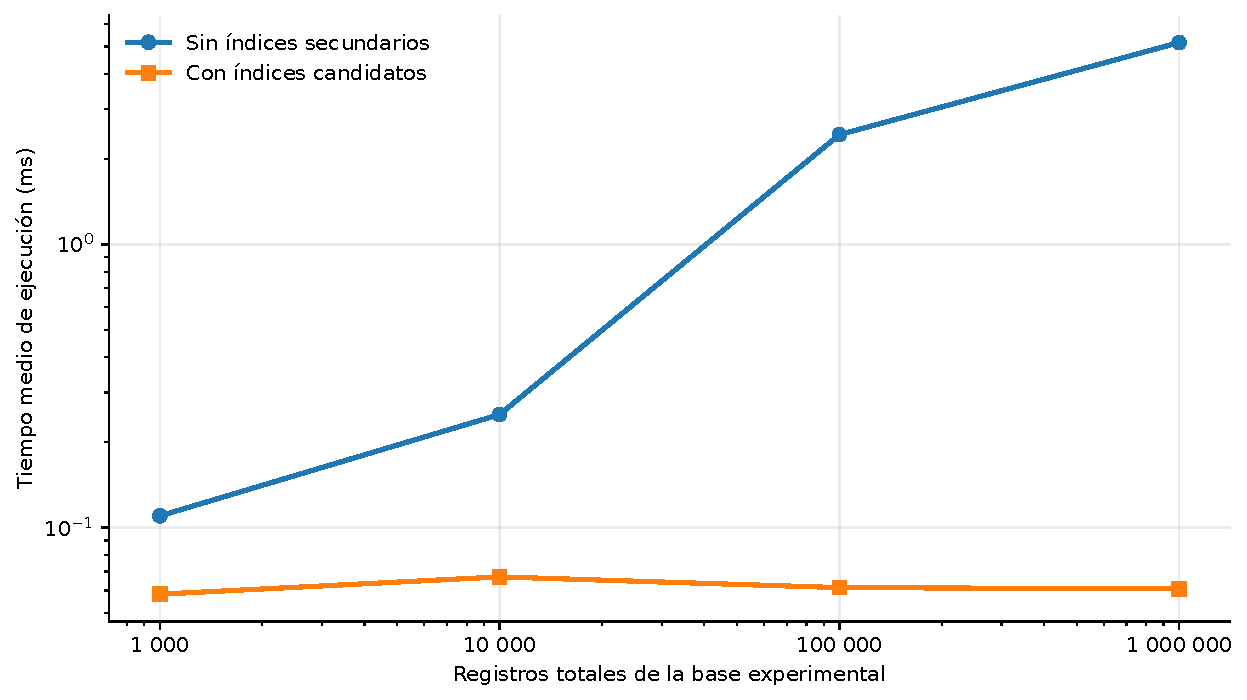
\includegraphics[width=0.94\textwidth,height=0.38\textheight,keepaspectratio]{figuras/grafico_C1.pdf}
\caption{C1: tiempo medio por volumen, sin índices secundarios y con el índice candidato.}
\label{fig:resultados-c1-56}
\end{figure}

En la escala de 1\,000 registros, PostgreSQL no empleó el índice
candidato (0/5). Aunque el escenario con el índice disponible registró
una media menor, esa diferencia no demuestra un beneficio del acceso
indexado. Desde 10\,000 registros el índice
se utilizó en las cinco mediciones de cada escala. En un millón, el
tiempo descendió de 5,1576 a 0,0608~ms (\textbf{98,82\,\% menos}).
Esta diferencia corresponde a los datos y filtros del experimento;
no debe generalizarse a toda distribución de eventos sísmicos.

\Needspace{0.57\textheight}
\subsubsection{Consulta 2: Eventos sísmicos en ventanas geográficas}
\begin{figure}[H]
\centering
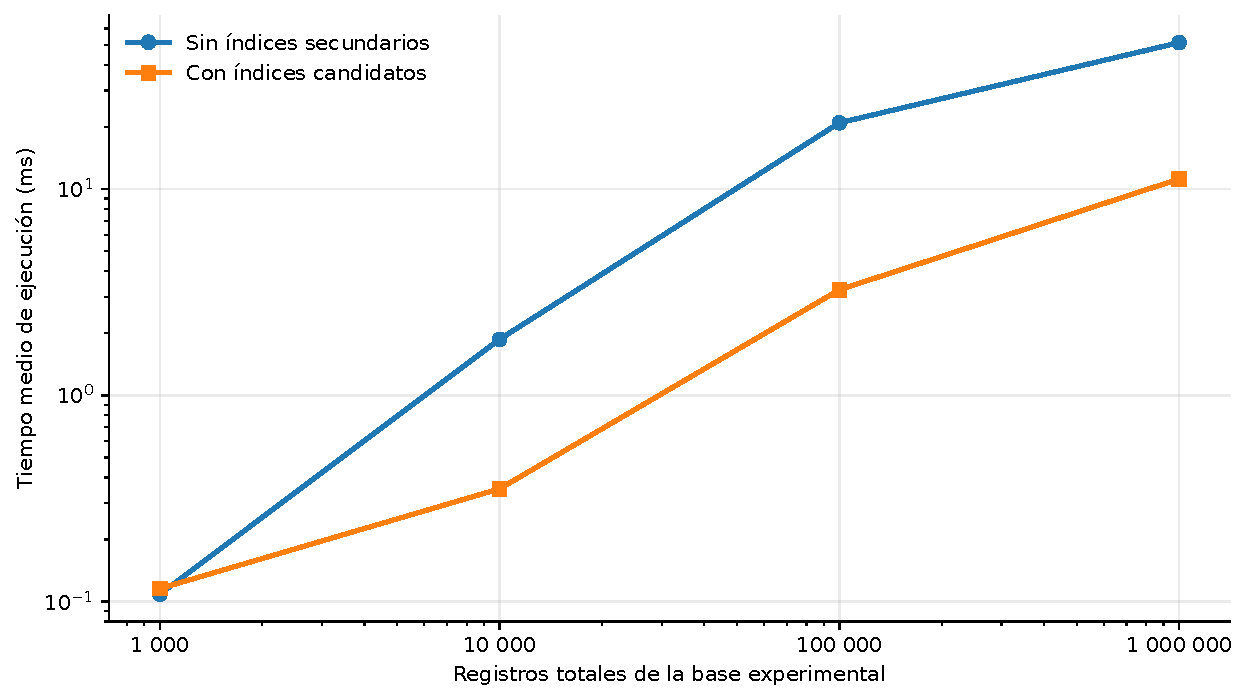
\includegraphics[width=0.94\textwidth,height=0.38\textheight,keepaspectratio]{figuras/grafico_C2.pdf}
\caption{C2: tiempos medios de la consulta espacial con y sin el índice candidato.}
\label{fig:resultados-c2-56}
\end{figure}

Con 1\,000 registros no se eligió el índice y la media fue ligeramente
mayor en el escenario indexado (0,1156 frente a 0,1086~ms). Desde
10\,000 registros hubo uso del índice en 5/5 mediciones, junto con
menores medias. Para un millón, la consulta pasó de 51,2426 a
11,1818~ms (\textbf{78,18\,\% menos}). La consulta emplea ventanas
rectangulares de latitud y longitud, no distancias geodésicas.

\Needspace{0.57\textheight}
\subsubsection{Consulta 3: Calidad de lecturas por estación}
\begin{figure}[H]
\centering
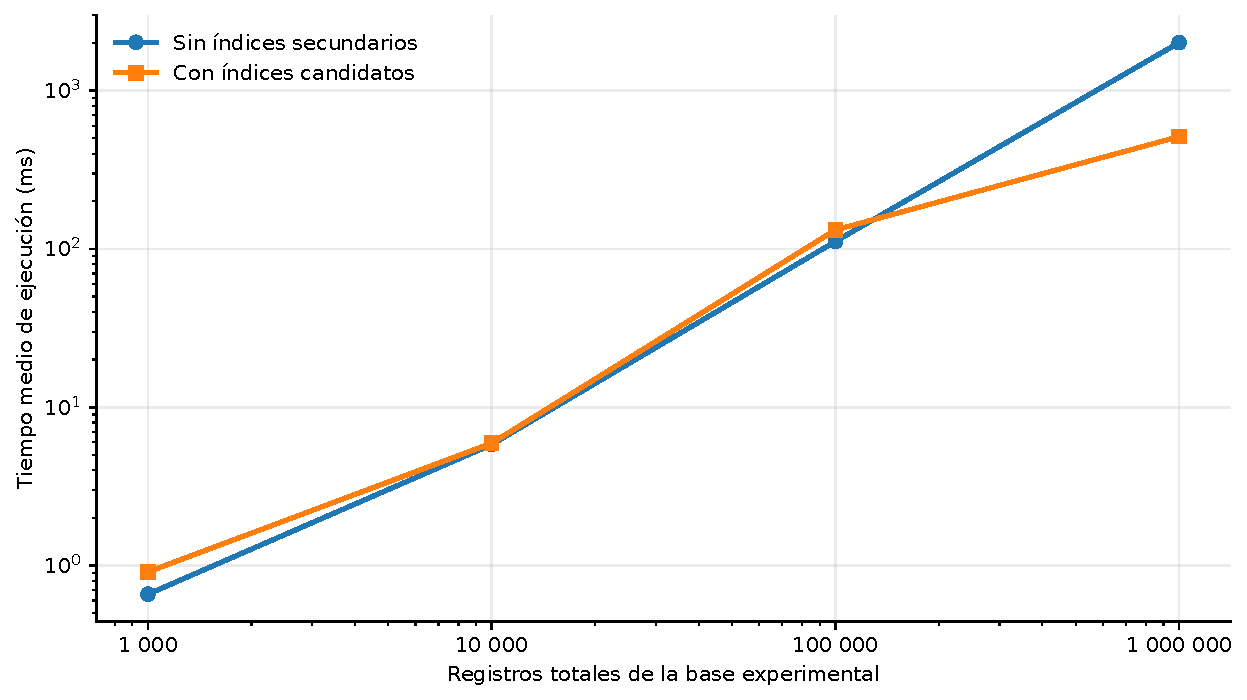
\includegraphics[width=0.94\textwidth,height=0.38\textheight,keepaspectratio]{figuras/grafico_C3.pdf}
\caption{C3: evolución del tiempo medio según el tamaño de la base.}
\label{fig:resultados-c3-56}
\end{figure}

El índice candidato no fue seleccionado en las tres escalas menores;
en ellas, las medias con el índice disponible fueron superiores a
las del escenario base. En un millón sí se utilizó (5/5), y la
media se redujo de 2\,013,4210 a 512,4504~ms
(\textbf{74,55\,\% menos}). El diagnóstico de la
Sección~\ref{sec:optimizacion-indices} documenta un cambio de plan
relevante para el ordenamiento; el beneficio de lectura debe
considerarse junto con el tamaño y mantenimiento del índice.

\Needspace{0.57\textheight}
\subsubsection{Consulta 4: Tiempos de primera detección y primera alerta}
\begin{figure}[H]
\centering
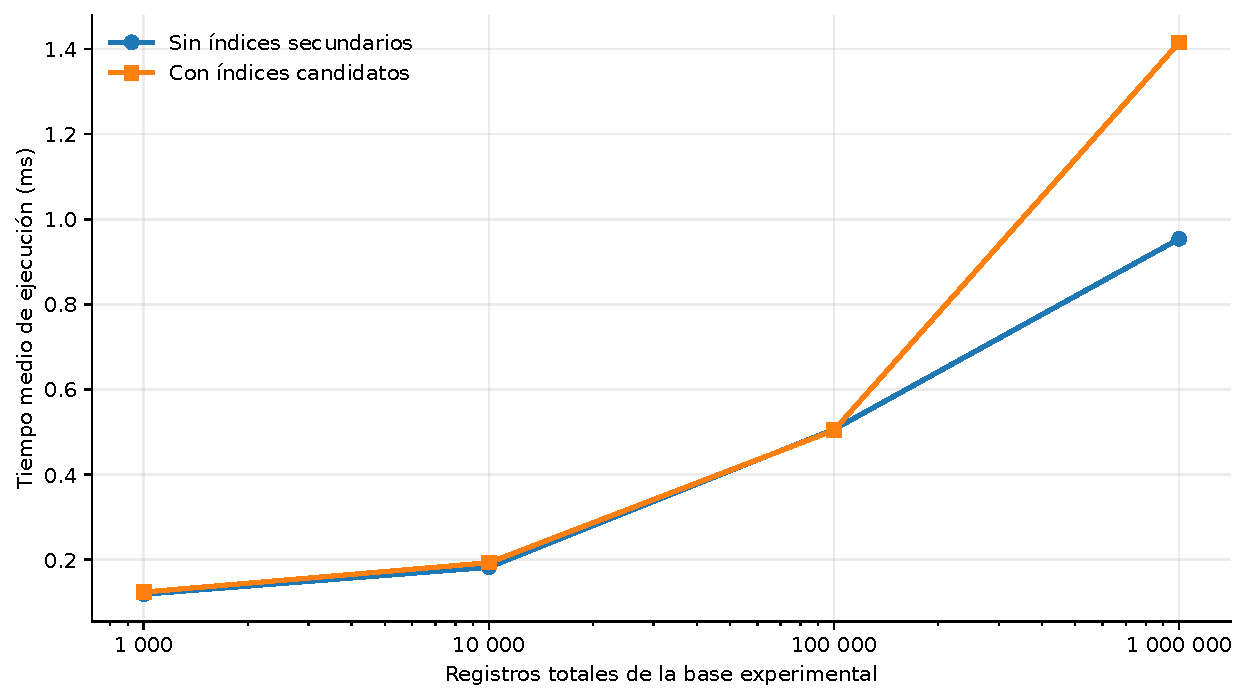
\includegraphics[width=0.94\textwidth,height=0.38\textheight,keepaspectratio]{figuras/grafico_C4.pdf}
\caption{C4: tiempos medios con los dos índices candidatos disponibles o ausentes.}
\label{fig:resultados-c4-56}
\end{figure}

PostgreSQL no utilizó ninguno de los dos índices candidatos en
ninguna escala (0/5 para ambos). En un millón, las medias fueron
0,9538 y 1,4148~ms sin y con los índices disponibles,
respectivamente: una diferencia absoluta de 0,4610~ms
(48,33\,\% más en el segundo escenario). Dado que ninguno se
seleccionó, \textbf{no corresponde atribuir esa diferencia al
acceso mediante los índices candidatos}.

\Needspace{0.57\textheight}
\subsubsection{Consulta 5: Sensores con lecturas y sin detecciones}
\begin{figure}[H]
\centering
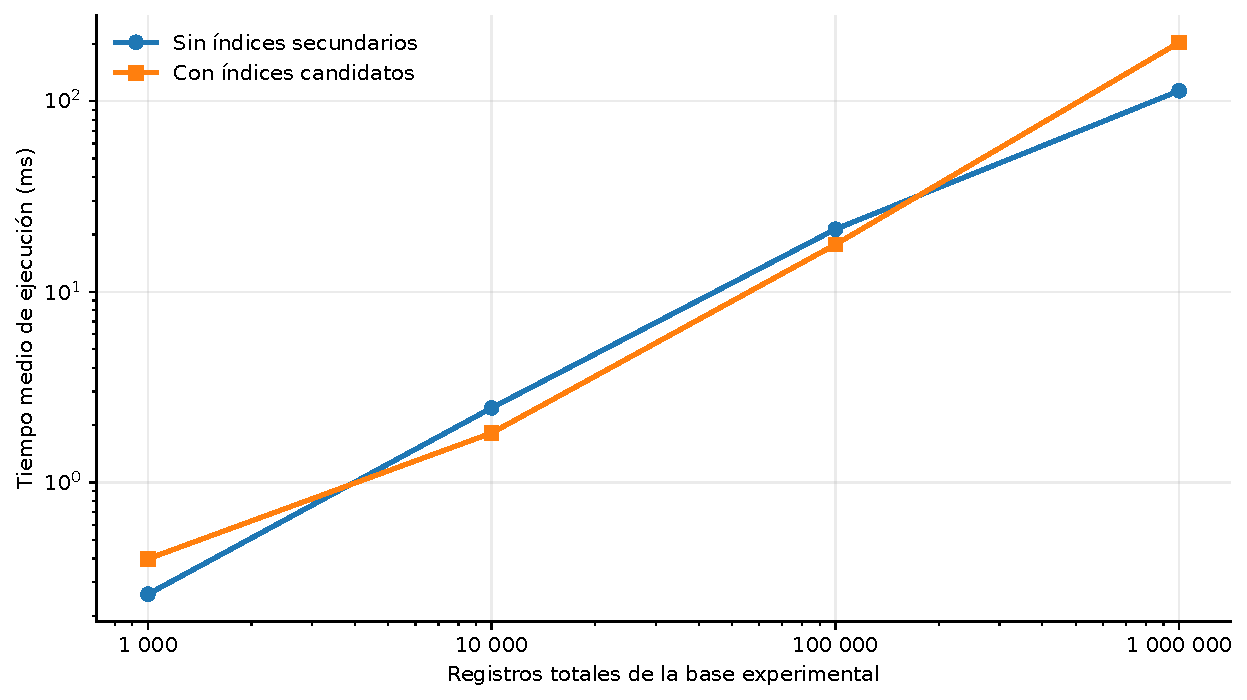
\includegraphics[width=0.94\textwidth,height=0.38\textheight,keepaspectratio]{figuras/grafico_C5.pdf}
\caption{C5: contraste de las medias y efecto no uniforme de la disponibilidad de índices.}
\label{fig:resultados-c5-56}
\end{figure}

Con 1\,000 registros, ninguno de los dos índices se utilizó y la
media fue mayor al tenerlos disponibles (0,3978 frente a
0,2596~ms). En 10\,000 registros se utilizó uno de ellos y la media
disminuyó 26,13\,\%; en 100\,000 se utilizaron ambos, con una
reducción de 16,86\,\%. Sin embargo, con un millón los dos índices
se usaron en 5/5 mediciones y la media aumentó de 113,3538 a
202,8902~ms (\textbf{78,99\,\% más}). Este caso demuestra que
la selección de índices no garantiza un menor tiempo de ejecución.

% =================================================
% 5.7 ANALISIS Y DISCUSION — REVISION PUNTUAL
% =================================================
\Needspace{0.52\textheight}
\subsection{Análisis y Discusión}
\label{sec:analisis-global-56}

\subsubsection{Balance de las veinte comparaciones y decisiones de indexación}
\label{sec:comparacion-global-56}
\label{sec:interpretacion-global-56}

Se evaluaron cinco consultas en cuatro escalas, bajo dos escenarios
por combinación. El protocolo contempló dos calentamientos y cinco
mediciones por escenario, con \textbf{200 mediciones registradas y 80
calentamientos} en total. La comprobación de equivalencia de
resultados se documenta en el procedimiento de medición.

El Cuadro~\ref{tab:resumen-global-56} sintetiza \emph{las decisiones
para la escala de un millón de registros}; las veinte comparaciones
y sus medidas descriptivas figuran en las Secciones~\ref{sec:medicion-tiempos}
y~\ref{sec:resultados-56}. Una variación negativa indica menor
media de ejecución en el escenario con índices. El uso corresponde
a las cinco mediciones de la serie principal, no a su mera existencia.

\begin{table}[H]
\centering\small
\setlength{\tabcolsep}{5pt}
\renewcommand{\arraystretch}{1.12}
\begin{tabular}{p{0.10\linewidth}p{0.17\linewidth}p{0.17\linewidth}p{0.40\linewidth}}
\toprule
\textbf{C} & \textbf{Uso efectivo} & \textbf{Variación} & \textbf{Implicación para la decisión} \\
\midrule
C1 & 5/5 & -98,82\,\% & Índice parcial favorable para el filtro estudiado. \\
C2 & 5/5 & -78,18\,\% & Índice geográfico favorable en esta distribución. \\
C3 & 5/5 & -74,55\,\% & Índice de cobertura útil a gran escala; evaluar su costo de mantenimiento. \\
C4 & 0/5 y 0/5 & +48,33\,\% & Ninguno de los dos índices fue elegido; no hay beneficio atribuible a ellos. \\
C5 & 5/5 y 5/5 & +78,99\,\% & Ambos se usaron, pero el plan resultó más lento en la serie principal. \\
\bottomrule
\end{tabular}

\caption{Síntesis de la indexación en la escala de un millón de registros (serie principal).}
\label{tab:resumen-global-56}
\end{table}

\textbf{Lectura del conjunto.} C1 y C2 utilizaron sus índices desde
10\,000 registros y fueron más rápidas en las tres escalas mayores.
En C3 el índice sólo se seleccionó con un millón de registros, cuando
el tiempo medio bajó de 2\,013,4210 a 512,4504~ms; su ocupación
aproximada de 34~MB debe considerarse junto con el costo de inserción
y actualización. C4 no utilizó ninguno de sus índices en ninguna
escala; su diferencia de tiempos no prueba un efecto de indexación.
C5, por último, mejoró en 10\,000 y 100\,000 registros, pero empeoró
en el millón aun utilizando ambos índices. \textbf{Utilización y
beneficio no son equivalentes}: la decisión debe basarse en el costo
del plan completo y en una carga de trabajo representativa.

\Needspace{0.30\textheight}
\subsubsection{Trazabilidad y alcance de las mediciones}
\label{sec:trazabilidad-series-57}

Las medias de la serie principal proceden del consolidado histórico
\nolinkurl{59_resumen_global_5_6.csv}. Sus desviaciones estándar
se conservan de los registros anteriores, ya que no se dispone
de las observaciones individuales necesarias para recalcularlas.

Una reejecución independiente generó veinte exportaciones previstas
por el integrador, cada una con cuatro calentamientos y diez
mediciones distribuidos entre los dos escenarios. El resumen
\nolinkurl{auditoria_dos_series_20_comparaciones.csv} identifica
los archivos locales y las firmas de resultados. No se adjuntan en
este informe las veinte series individuales de la reejecución; el
integrador \texttt{06\_mediciones.sql} permite regenerarlas.

Por ejemplo, para C5 con un millón de registros, las medias de la
serie principal fueron 113,3538 y 202,8902~ms (sin y con índices),
mientras que la reejecución registró 110,3134 y 117,3334~ms.
\textbf{Las dos series se analizan por separado}: no se promedian
entre sí ni se atribuyen sus diferencias a una causa no verificada.
No se afirma significancia estadística a partir de cinco mediciones
por condición.

\subsubsection{Análisis adicional: crecimiento más allá del millón}
\label{sec:extra-escalabilidad}

Se examina el posible comportamiento del sistema por encima del millón
de registros y la suficiencia de la arquitectura
cliente--servidor. \textbf{El mayor tamaño construido y medido fue de
1\,000\,000 de filas}; no se ejecutaron consultas sobre diez millones.
Para disponer de una referencia cuantitativa, la
Cuadro~\ref{tab:extra-distribucion-10m} multiplica \emph{hipotéticamente}
por diez la composición de la base máxima. No es una predicción del
crecimiento real del catálogo del IGP ni una medición de rendimiento.

\begin{table}[H]
\centering\small
\begin{tabular}{lrr}
\toprule
\textbf{Relación} & \textbf{1 millón: medido} & \textbf{10 millones: supuesto} \\
\midrule
\texttt{estacion\_sismica} & 100 & 1\,000 \\
\texttt{sensor} & 300 & 3\,000 \\
\texttt{evento\_sismico} & 120\,000 & 1\,200\,000 \\
\texttt{lectura\_onda} & 875\,000 & 8\,750\,000 \\
\texttt{deteccion} & 3\,500 & 35\,000 \\
\texttt{alerta} & 1\,100 & 11\,000 \\
\midrule
\textbf{Total} & \textbf{1\,000\,000} & \textbf{10\,000\,000} \\
\bottomrule
\end{tabular}

\caption{Volumen verificado y ejemplo hipotético de crecimiento proporcional.}
\label{tab:extra-distribucion-10m}
\end{table}

El crecimiento afectaría de forma distinta a cada consulta. En C1,
la selectividad del filtro temporal determinaría cuánto aporta el
índice parcial. En C2, las búsquedas por rangos de latitud y longitud
pueden producir numerosos candidatos aun usando un índice compuesto.
C3 depende principalmente del volumen de lecturas que debe agrupar;
C4 resume detecciones y alertas, por lo que un recorrido amplio puede
seguir siendo preferible a búsquedas indexadas. En C5, la anti-unión
y las búsquedas reiteradas por sensor pueden aumentar el costo incluso
cuando PostgreSQL utiliza los índices propuestos.

\textbf{No sería válido multiplicar por diez los milisegundos
observados}: pueden cambiar el plan, la tasa de aciertos en caché,
los accesos a disco y la concurrencia. En particular, el caso C5
muestra que incluso un plan que utiliza índices puede ser más lento
que el plan sin ellos. Este análisis no supone que los 24\,289
eventos reales del catálogo IGP se multiplicarán automáticamente;
se requerirían nuevas fuentes verificadas o datos sintéticos
identificados como tales.

\textbf{¿Es suficiente cliente--servidor?} PostgreSQL 18.6 respondió
las cinco consultas con un millón de registros en el equipo descrito
en 5.4. Esto respalda una arquitectura cliente--servidor como punto
de partida, \textbf{no garantiza} latencias aceptables con diez
millones ni con múltiples usuarios. Antes de cambiar de arquitectura
correspondería (i) medir consultas y escrituras concurrentes con
\texttt{EXPLAIN (ANALYZE, BUFFERS)} y estadísticas actualizadas,
(ii) revisar índices y reescrituras de consultas, especialmente C5,
y (iii) evaluar particionamiento temporal, vistas materializadas o
más recursos únicamente si aparecen cuellos de botella medidos.
Las referencias técnicas utilizadas son la documentación de
\url{https://www.postgresql.org/docs/18/using-explain.html} y de
\url{https://www.postgresql.org/docs/18/ddl-partitioning.html}.

\subsubsection{Limitaciones y reproducibilidad}
\label{sec:limitaciones-global-56}

Las comparaciones se realizaron en un orden fijo (primero sin y
luego con índices) y con sólo cinco mediciones válidas por condición.
Los calentamientos, la caché y las distintas selectividades de las
cuatro bases pueden influir en los tiempos; \texttt{shared hit} y
\texttt{shared read} son contadores de búferes, no mediciones directas
de operaciones físicas de disco. Los resultados son, por tanto,
\textbf{descriptivos para esta carga y plataforma}, no una prueba
causal o universal del beneficio de un índice.

Los cuatro archivos \texttt{.dump} se conservaron antes de crear los
índices experimentales. Está documentada la restauración de la base
de 1\,000 registros en
\nolinkurl{bd_sismologico_restauracion_1000}, incluidos sus recuentos
y controles de integridad; \textbf{no equivale a comprobar la
restauración de los otros tres respaldos}. Los árboles reales de ejecución se presentan mediante extractos
en la Sección~\ref{sec:optimizacion-indices}; los diez SVG íntegros
se conservan como respaldo. Esas verificaciones visuales posteriores
no sustituyen las mediciones repetidas de la serie principal.

% =================================================
% 6. CONCLUSIONES
% =================================================
\clearpage
\section{Conclusiones}

\begin{enumerate}[leftmargin=*,label=\arabic*.,itemsep=0.65em,parsep=0pt]
    \item \textbf{Implementación e integridad.} Se implementó en PostgreSQL un esquema de seis tablas consistente con el modelo relacional, con claves y restricciones de integridad. Las cinco vistas, seis procedimientos almacenados y nueve disparadores permiten consultar y controlar operaciones sobre el dominio sismológico. Las pruebas documentadas respaldan las reglas verificadas, sin extender ese resultado a todos los casos posibles.

    \item \textbf{Procedencia y volumen de los datos.} Se integraron 24\,289 eventos del catálogo oficial del Instituto Geofísico del Perú y registros operativos simulados, identificando claramente su procedencia. Se construyeron cuatro bases experimentales de 1\,000, 10\,000, 100\,000 y 1\,000\,000 de registros, sin presentar los datos sintéticos como observaciones sismológicas reales.

    \item \textbf{Optimización condicionada por la carga.} En la serie principal, los índices candidatos de C1 y C2 se utilizaron y mejoraron los tiempos desde 10\,000 registros. En C3, el índice sólo fue utilizado en la escala de un millón, donde la media disminuyó de 2\,013,4210 a 512,4504~ms (74,55\,\%). Los resultados evidencian que la utilidad de cada índice depende de la consulta, el volumen y el plan elegido por PostgreSQL.

    \item \textbf{Ausencia de mejora automática.} C4 no utilizó sus índices candidatos en ninguna escala, por lo que la diferencia temporal observada no demuestra un beneficio de indexación. En C5, ambos índices fueron utilizados con un millón de registros, pero la media aumentó de 113,3538 a 202,8902~ms (78,99\,\%). La utilización de índices no equivale necesariamente a menor tiempo de respuesta.

    \item \textbf{Alcance de la experimentación.} Se realizaron dos calentamientos y cinco mediciones por escenario en cada una de las veinte combinaciones de consulta y escala. Los tiempos son descriptivos para el equipo y los datos utilizados: el orden fijo de los escenarios, los efectos de caché y la falta de mediciones individuales de la primera serie limitan las inferencias. Las reejecuciones se mantienen separadas del consolidado principal.

    \item \textbf{Validación del prototipo web.} El MVP de consulta en modo de sólo lectura se conectó localmente a la base experimental de un millón de registros y permitió ejecutar C1--C5 desde una interfaz web. Esta prueba demuestra integración funcional en el entorno utilizado, pero no constituye una validación de despliegue público, concurrencia o latencia de un sistema de alerta temprana real.

    \item \textbf{Reproducibilidad y crecimiento.} Se publicaron cuatro respaldos experimentales y se documentó la restauración independiente del de 1\,000 registros; no se verificó individualmente la restauración de los otros tres. El mayor volumen evaluado fue de un millón de registros. La operación con diez millones o con múltiples usuarios requiere pruebas adicionales antes de formular conclusiones sobre escalabilidad o infraestructura.
\end{enumerate}
\clearpage

% =================================================
% 7. ANEXOS
% =================================================
\section{Anexos}

\subsection{Código fuente y reproducibilidad de la implementación}

La implementación está disponible en el
\href{https://github.com/FabricioNick/Sistema-Monitoreo-Sismologico}{repositorio del proyecto}.
Se organiza en siete integradores SQL que permiten reproducir la
estructura relacional, la carga de datos, la lógica de negocio y los
experimentos de rendimiento.

\begin{table}[H]
\centering\small
\begin{tabular}{>{\raggedright\arraybackslash}p{6.0cm}>{\raggedright\arraybackslash}p{7.1cm}}
\toprule
\textbf{Integrador} & \textbf{Responsabilidad} \\
\midrule
\nolinkurl{01_estructura.sql} & Tablas, claves, restricciones y comprobaciones de integridad. \\
\nolinkurl{02_datos.sql} & Carga del catálogo IGP, datos complementarios y verificaciones. \\
\nolinkurl{03_logica_consultas.sql} & Vistas, procedimientos, triggers y cinco consultas intermedias. \\
\nolinkurl{04_bases_experimentales.sql} & Preparación y validación de las cuatro escalas experimentales. \\
\nolinkurl{05_planes_indices.sql} & Planes de ejecución y evaluación de índices por consulta. \\
\nolinkurl{06_mediciones.sql} & Mediciones repetidas y controles de equivalencia de resultados. \\
\nolinkurl{07_demostracion_video.sql} & Demostración reproducible en la escala de un millón de registros. \\
\bottomrule
\end{tabular}

\caption{Integradores definitivos utilizados como referencia técnica del proyecto.}
\label{tab:integradores-definitivos}
\end{table}

Para reproducir la implementación se utiliza \texttt{psql} y, en la
etapa de carga, el CSV oficial del IGP obtenido de la fuente indicada
en el repositorio. El integrador 07 presupone el estado de índices
C5 generado por las pruebas finales; no se ejecuta directamente
sobre un respaldo recién restaurado sin preparar dicho estado.

El archivo \nolinkurl{59_resumen_global_5_6.csv} contiene las
veinte comparaciones de la serie principal. La segunda serie
experimental consta en \nolinkurl{auditoria_dos_series_20_comparaciones.csv}
y se analizó por separado, sin combinar sus medias con las de la
serie principal.

\subsection{Respaldo de las cuatro bases experimentales}

Se generaron cuatro respaldos en formato personalizado mediante
\texttt{pg\_dump -Fc} tras verificar los recuentos
e integridad de cada base. Los archivos conservan el estado anterior a
la incorporación de los índices secundarios de las pruebas de rendimiento.
Los cuatro respaldos están publicados como archivos adjuntos
de la \href{https://github.com/FabricioNick/Sistema-Monitoreo-Sismologico/releases/tag/v1.0.0}{versión v1.0.0}
en GitHub Releases.

\begin{table}[H]
\centering\small
\begin{tabular}{ll}
\toprule
\textbf{Escala} & \textbf{Archivo de respaldo} \\
\midrule
1\,000 & \nolinkurl{bd_sismologico_exp_1000.dump} \\
10\,000 & \nolinkurl{bd_sismologico_exp_10000.dump} \\
100\,000 & \nolinkurl{bd_sismologico_exp_100000.dump} \\
1\,000\,000 & \nolinkurl{bd_sismologico_exp_1000000.dump} \\
\bottomrule
\end{tabular}
\caption{Respaldos de las cuatro bases experimentales publicados en la versión v1.0.0.}
\label{tab:respaldos-experimentales}
\end{table}

\textbf{Restauración independiente verificada.} La prueba de
restauración y la verificación de integridad se ejecutaron sobre el respaldo
\nolinkurl{bd_sismologico_exp_1000.dump}, sin sobrescribir
las bases experimentales. El procedimiento terminó correctamente.\space\texttt{pg\_restore} reconoció el archivo en formato personalizado
y finalizó sin errores dentro de una única transacción. La
restauración se realizó sobre la base independiente
\nolinkurl{bd_sismologico_restauracion_1000}.

\begin{table}[H]
\centering\small
\begin{tabular}{lrrl}
\toprule
\textbf{Relación} & \textbf{Esperado} & \textbf{Restaurado} & \textbf{Control} \\
\midrule
\texttt{estacion\_sismica} & 5 & 5 & OK \\
\texttt{sensor} & 15 & 15 & OK \\
\texttt{evento\_sismico} & 100 & 100 & OK \\
\texttt{lectura\_onda} & 750 & 750 & OK \\
\texttt{deteccion} & 90 & 90 & OK \\
\texttt{alerta} & 40 & 40 & OK \\
\midrule
\textbf{Total} & \textbf{1\,000} & \textbf{1\,000} & \textbf{OK} \\
\bottomrule
\end{tabular}

\caption{Recuentos de relaciones tras restaurar el respaldo de 1\,000 registros.}
\label{tab:restauracion-verificada-1000}
\end{table}

El verificador informó \textbf{50 eventos del IGP y 50 eventos
sintéticos}, \textbf{9 triggers} y \textbf{cero incumplimientos}
en los cuatro controles: estaciones sin sensores, detecciones
sin lectura válida, alertas anteriores a su evento y lecturas
válidas de sensores inoperativos. Además, no se encontraron
detecciones ni alertas vinculadas a los eventos reales del IGP.
La copia restaurada ocupó \textbf{8\,534 kB} al finalizar.

El script reportó para el archivo original la siguiente huella
\textbf{SHA-256}, útil para comprobar su identidad:
\begin{center}
\footnotesize\ttfamily
FDB9280617F3B20CD3229B671CD8AF06\\
ADFD08094E3F4003A13FA786B42D90F7
\end{center}

La salida terminó con el aviso \emph{«OK: respaldo restaurado
y verificado en base independiente»} y confirmó que las bases
\nolinkurl{bd_sismologico_exp_1000},
\nolinkurl{bd_sismologico_exp_10000},
\nolinkurl{bd_sismologico_exp_100000} y
\nolinkurl{bd_sismologico_exp_1000000} no fueron alteradas.
\textbf{Alcance:} este resultado certifica la recuperación del
respaldo de 1\,000 registros; la recuperación de los otros tres
archivos todavía no se ha comprobado individualmente.

\Needspace{0.33\textheight}
\subsection{Demostración SQL sobre un millón de registros}

\textbf{Ejecución demostrativa.} Se ejecutó
\texttt{sql/07\_demostracion\_video.sql} sobre
\nolinkurl{bd_sismologico_exp_1000000}. El control inicial verificó
la distribución de \textbf{1\,000\,000 de registros} en seis tablas
y la presencia exclusiva de los dos índices secundarios de C5.
Se ejecutó una vez cada consulta en ambos escenarios; los diez
resultados figuran en el Cuadro~\ref{tab:video-demostracion-62}.

\begin{table}[H]
\centering\small
\setlength{\tabcolsep}{6pt}
\begin{tabular}{lrrl}
\toprule
\textbf{Consulta} & \textbf{Sin índice} & \textbf{Con índice} & \textbf{Índice candidato usado} \\
\midrule
C1 & 13,690 & 0,105 & Sí, parcial \\
C2 & 46,298 & 11,090 & Sí, geográfico \\
C3 & 1\,819,563 & 567,325 & Sí, cobertura \\
C4 & 1,543 & 1,435 & Ninguno \\
C5 & 107,379 & 231,111 & Ambos \\
\bottomrule
\end{tabular}

\caption{Tiempos de la ejecución demostrativa del integrador 07, con un millón de registros (ms).}
\label{tab:video-demostracion-62}
\end{table}

La demostración de C3 informó \textbf{7\,501 bloques temporales leídos}
y \textbf{7\,516 escritos} en el plan sin índice, frente a cero en
el plan indexado. En C4, los dos índices candidatos no fueron usados.
En C5, ambos se utilizaron, aunque el tiempo demostrativo fue mayor
con ellos. Los diez tiempos anteriores corresponden a \emph{una
sola ejecución por escenario}; no reemplazan las medias de cinco
mediciones de la Sección~\ref{sec:medicion-tiempos}.

Al finalizar, el archivo devolvió \texttt{ROLLBACK} y una consulta
posterior confirmó que permanecían exclusivamente los índices
\nolinkurl{idx_det_sensor_hora_c5} y
\nolinkurl{idx_lectura_sensor_hora_c5}. Por tanto, la demostración
SQL y el restablecimiento del estado original quedaron \textbf{verificados}.


\medskip
\noindent\textbf{Organización de la evidencia audiovisual.}
La evidencia audiovisual se organiza en un único recorrido por la base
\nolinkurl{bd_sismologico_exp_1000000}: verificación de los seis recuentos,
consultas C1--C5 sin índices secundarios y con índices candidatos, lectura de
\texttt{Execution Time} y verificación final de la restauración del estado
mediante \texttt{ROLLBACK}. Las diez condiciones se identifican mediante
marcas de tiempo para facilitar su consulta, sin sustituir las cinco
mediciones repetidas de cada escenario presentadas en el informe.
La carpeta de acceso a la evidencia audiovisual es
\href{https://drive.google.com/drive/folders/1gb3Di7rx0eWwd05cC3xbw3DJxhjgS2t4?usp=sharing}{Video de experimentación en Google Drive}.

\Needspace{0.26\textheight}
\subsection{Prototipo web de consultas}
\label{sec:anexo-mvp-web}

Se preparó el código fuente de \nolinkurl{MVP_Web_Sismologico},
una aplicación web de consulta que integra un servidor HTTP en
\texttt{Node.js}, el controlador \texttt{pg} y una interfaz HTML,
CSS y JavaScript. El servidor se conecta a PostgreSQL a través
de la configuración privada \texttt{.env}; el navegador no recibe
la contraseña. La implementación utiliza las cinco sentencias
\texttt{SELECT} del integrador \texttt{03\_logica\_consultas.sql}, sin alterar
sus filtros ni los identificadores correctos de la Consulta 4.

La interfaz incorpora una pantalla de bienvenida y un menú lateral plegable, que facilita la visualización de resultados en pantallas de distinta anchura. Permite visualizar los recuentos de las seis tablas,
seleccionar cualquiera de las cinco consultas intermedias,
inspeccionar los resultados en una tabla, filtrar, ordenar,
representar una métrica y exportar las filas visibles a CSV.
Los servicios disponibles son
\texttt{GET /api/health}, \texttt{GET /api/overview},
\texttt{GET /api/queries} y
\texttt{GET /api/queries/C1} hasta \texttt{C5}.
Las consultas se ejecutan mediante transacciones
\texttt{BEGIN READ ONLY}, con tiempo máximo configurado y
\texttt{ROLLBACK} al terminar. No se admiten sentencias SQL
arbitrarias proporcionadas por el navegador ni operaciones
de inserción, actualización o eliminación.

\textbf{Validación técnica y funcional.} Se verificó la sintaxis
del servidor y del cliente, se contrastaron las cinco sentencias
SQL con su fuente original y se aprobaron pruebas automatizadas
del manejo HTTP y del modo de solo lectura mediante un controlador
simulado. Posteriormente, se inició la aplicación en el equipo
local y se confirmó la conexión con
\nolinkurl{bd_sismologico_exp_1000000}, la base experimental
realizada en PostgreSQL con exactamente 1\,000\,000 de registros.
El panel mostró 24\,289 eventos provenientes del archivo del IGP,
875\,000 lecturas y 300 sensores; dichas cantidades coincidieron
con las verificaciones SQL de la base experimental.

\textbf{Resultados de las consultas desde la interfaz web.}
Las pruebas locales permitieron observar los resultados de C1--C4
y exportar la respuesta de C5 a un archivo CSV. Se obtuvieron los
siguientes resultados:

\begin{table}[H]
\centering
\small
\renewcommand{\arraystretch}{1.16}
\begin{tabular}{>{\raggedright\arraybackslash}p{2.0cm} c
                >{\raggedright\arraybackslash}p{3.1cm}
                >{\raggedright\arraybackslash}p{6.0cm}}
\toprule
\textbf{Consulta} & \textbf{Filas} & \textbf{Respuesta web} & \textbf{Resultado observado} \\
\midrule
C1 & 15 & 8,95 ms & Actividad sísmica anual agrupada. \\
C2 & 10 & 286,21 ms & Eventos clasificados por ventana geográfica. \\
C3 & 100 & 332,59 ms & Indicadores de validez de lecturas por estación. \\
C4 & 15 & 7,96 ms & Detecciones y alertas de eventos simulados. \\
C5 & 15 & 185,14 ms & Exportación CSV: 15 sensores distintos, 43\,755 lecturas y 2\,580 lecturas inválidas. \\
\bottomrule
\end{tabular}
\caption{Resultados de las consultas C1--C5 desde el prototipo web local.}
\label{tab:resultados-mvp-web}
\end{table}

El archivo \nolinkurl{C5_resultados_mvp.csv} fue comprobado:
contiene 15 registros con 15 identificadores de sensor distintos,
y las sumas de las columnas de lecturas e inválidas corresponden
a los totales de la Consulta 5 documentados en la experimentación.
Las cinco consultas demostraron funcionamiento conectado a la base
local, con acceso \texttt{READ ONLY}, y se verificó también la
exportación de resultados a CSV.

Los tiempos de \emph{respuesta del servidor} de la aplicación web
no se equiparan directamente con \texttt{Execution Time} de
\texttt{EXPLAIN ANALYZE}: corresponden a mecanismos de medición
y capas de ejecución diferentes. Los tiempos de detección y
alerta observados en C4 proceden de registros simulados y no
constituyen una evaluación de latencia operativa de un sistema
público de alerta temprana.



\clearpage
\begin{figure}[H]
\centering
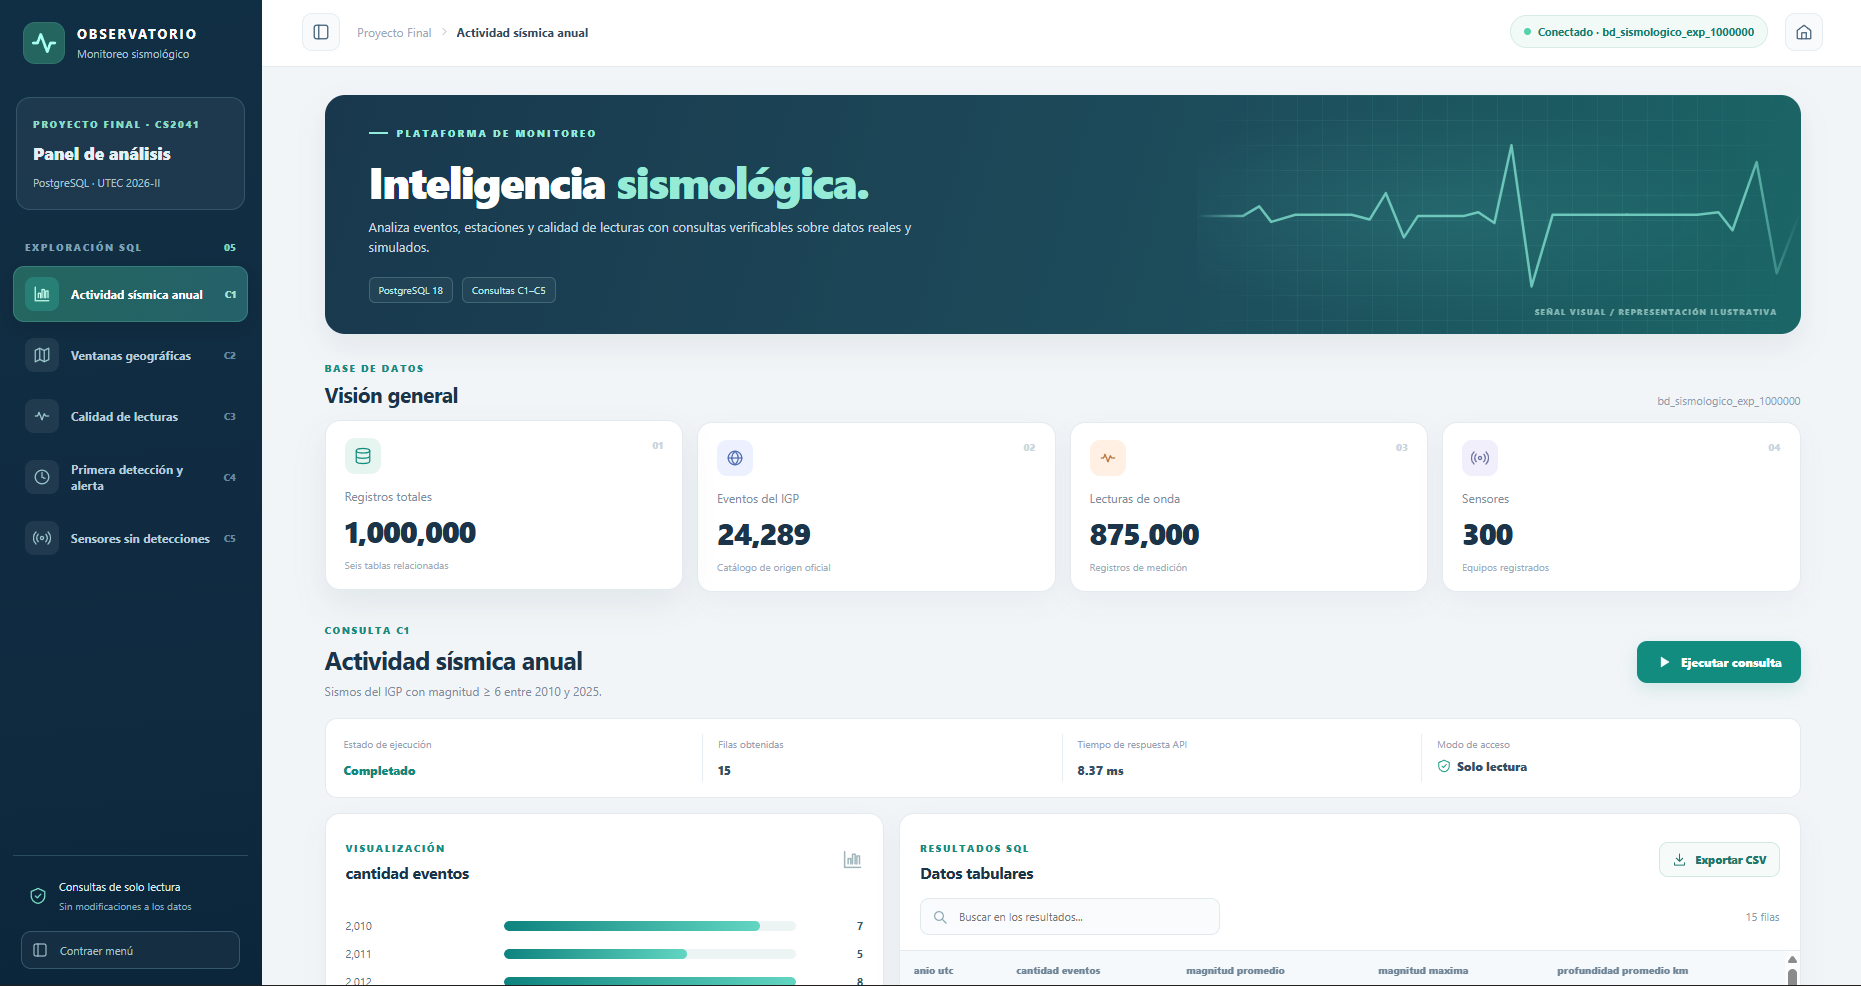
\includegraphics[width=0.98\linewidth,height=0.63\textheight,keepaspectratio]{figuras/captura_MVP_panel_principal.png}
\caption{Panel principal del MVP web, conectado a la base experimental de un millón de registros. Se muestran el resumen de la base y la consulta C1 ejecutada.}
\label{fig:mvp-panel-final}
\end{figure}

\begin{figure}[H]
\centering
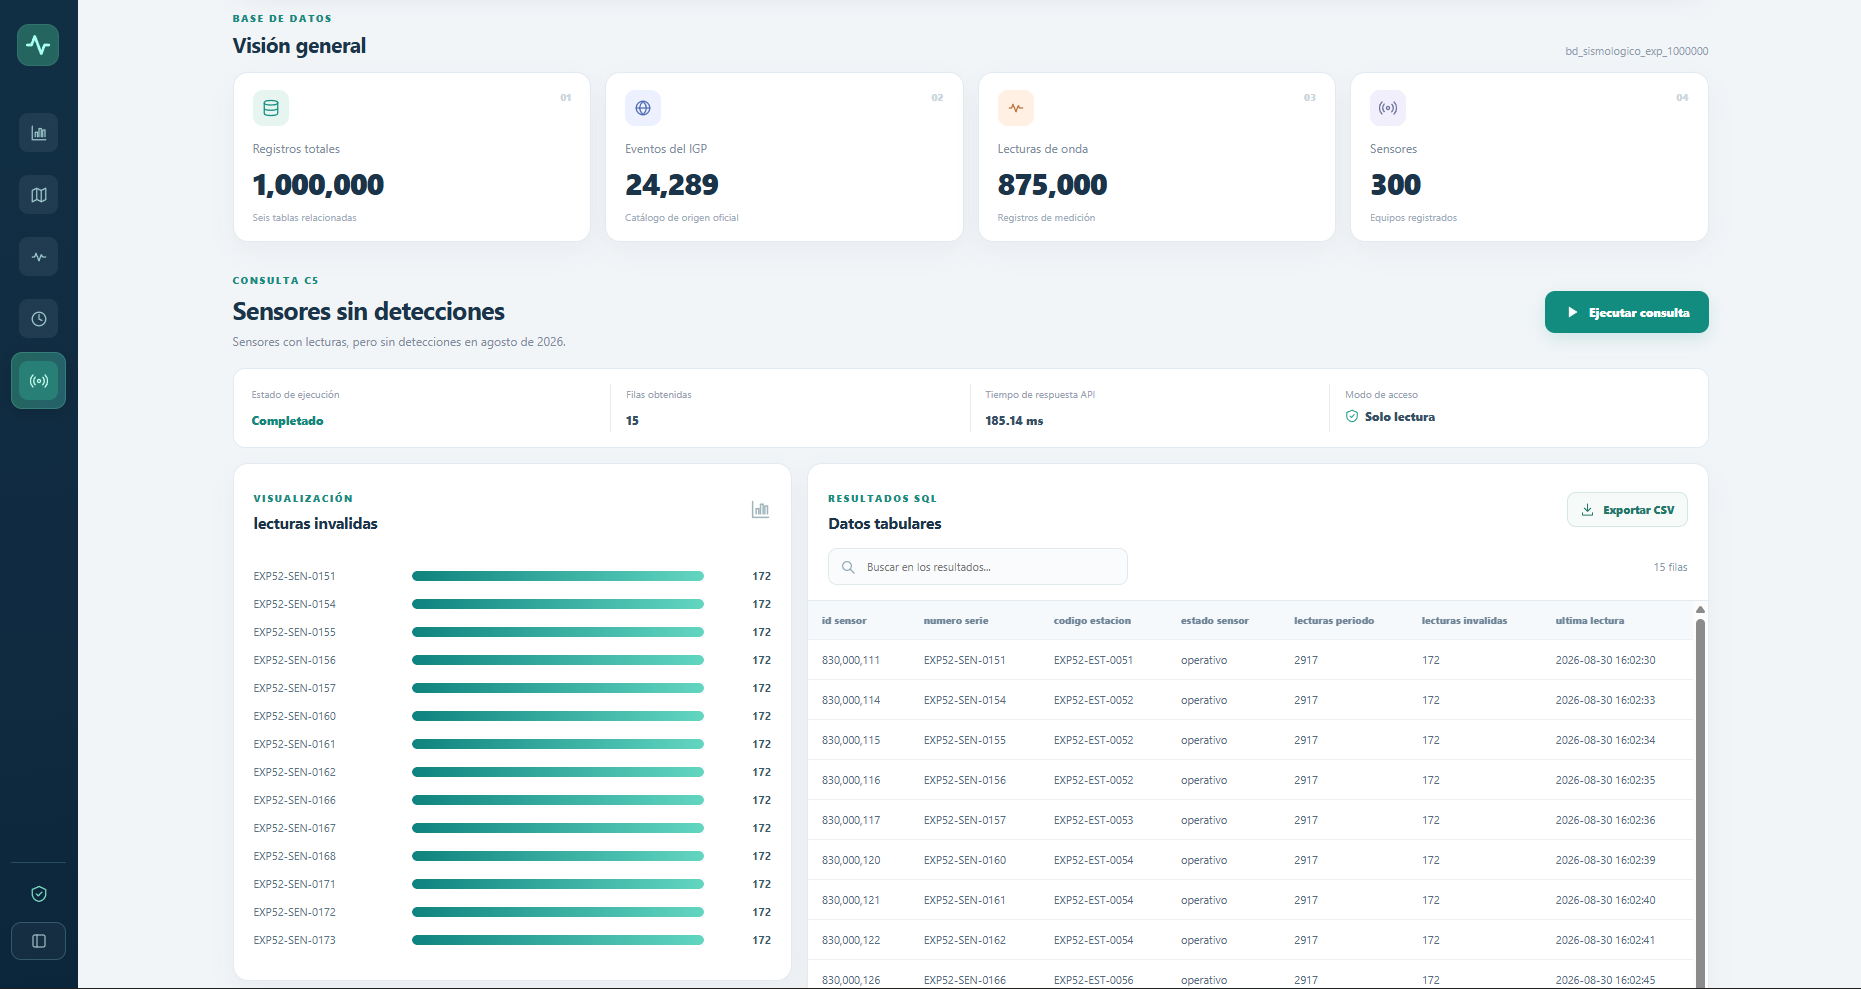
\includegraphics[width=0.98\linewidth,height=0.71\textheight,keepaspectratio]{figuras/captura_MVP_consulta_C5.png}
\caption{Consulta C5 ejecutada en el MVP, con quince sensores identificados, visualización de lecturas inválidas y tabla de resultados.}
\label{fig:mvp-c5-final}
\end{figure}




\clearpage
\subsection{Verificación tabular de la consulta geográfica}
\label{sec:anexo-c2}
La Figura~\ref{fig:c2-pgadmin-complementaria} registra la ejecución
original de C2 en la base temporal de comprobación
\nolinkurl{bd_sismologico_prueba_exp_1000000}, distinta de la
base experimental principal, con las diez filas devueltas por la
consulta y los campos de identificación, cantidad de eventos y magnitudes.

\begin{figure}[H]
\centering
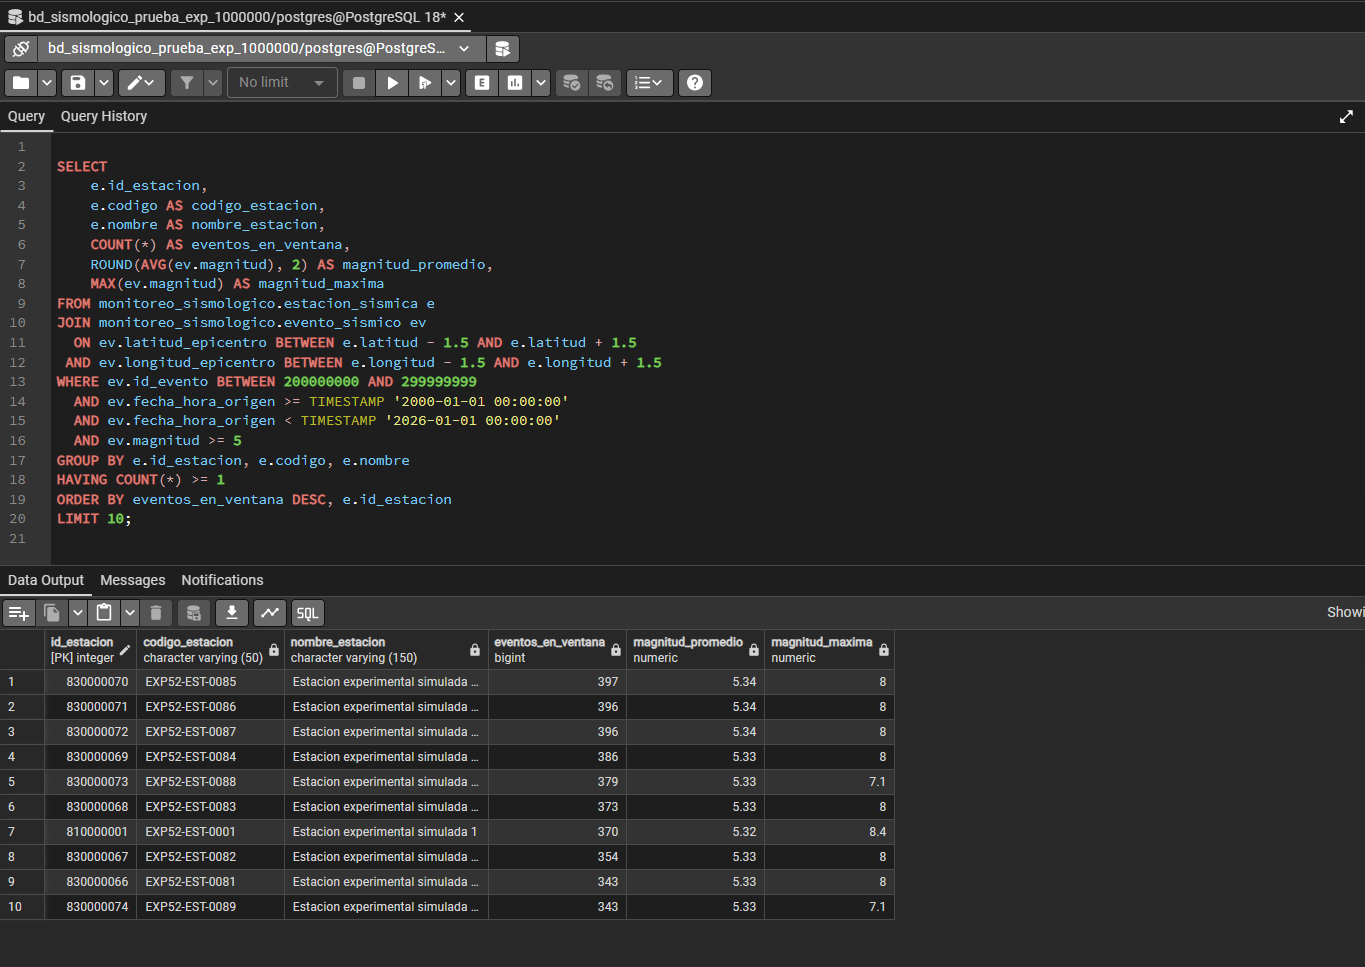
\includegraphics[width=0.99\linewidth,height=0.80\textheight,keepaspectratio]{figuras/captura_C2_base_prueba_pgadmin.png}
\caption{Consulta C2 en pgAdmin: resultados de ventanas geográficas en una copia de prueba de la escala de un millón de registros.}
\label{fig:c2-pgadmin-complementaria}
\end{figure}

\clearpage
\subsection{Código SQL de la implementación y los experimentos}
\label{sec:anexo-codigo-integro}
Los siguientes listados reúnen los integradores SQL de la estructura,
carga de datos, lógica de negocio, experimentación y demostración.
Los fundamentos de las operaciones y el análisis de resultados se desarrollan
en los Capítulos 4 y 5. El repositorio contiene los módulos complementarios
y los archivos de resultados correspondientes.

\begingroup
\setlength{\parskip}{0.25em}

\subsubsection{Estructura y restricciones}
\lstinputlisting[style=sqlanexo,caption={Integrador 01: estructura y restricciones.},label={lst:full-01}]{../sql/01_estructura.sql}

\subsubsection{Carga, catálogo IGP y simulación}
\lstinputlisting[style=sqlanexo,caption={Integrador 02: carga y verificación de datos.},label={lst:full-02}]{../sql/02_datos.sql}

\subsubsection{Vistas, procedimientos, disparadores y consultas}
\lstinputlisting[style=sqlanexo,caption={Integrador 03: lógica de negocio y consultas C1--C5.},label={lst:full-03}]{../sql/03_logica_consultas.sql}

\subsubsection{Bases experimentales}
\lstinputlisting[style=sqlanexo,caption={Integrador 04: preparación de las cuatro escalas.},label={lst:full-04}]{../sql/04_bases_experimentales.sql}

\subsubsection{Planes de ejecución e índices}
\lstinputlisting[style=sqlanexo,caption={Integrador 05: planes y candidatos de indexación.},label={lst:full-05}]{../sql/05_planes_indices.sql}

\subsubsection{Medición de rendimiento}
\lstinputlisting[style=sqlanexo,caption={Integrador 06: protocolo de mediciones por escala.},label={lst:full-06}]{../sql/06_mediciones.sql}

\subsubsection{Demostración de la escala máxima}
\lstinputlisting[style=sqlanexo,caption={Integrador 07: acceso a la demostración.},label={lst:full-07}]{../sql/07_demostracion_video.sql}
\lstinputlisting[style=sqlanexo,caption={Módulo 62: demostración reversible de las consultas C1--C5.},label={lst:full-62}]{../sql/modulos/demostracion/62_demostracion_video_1000000.sql}
\endgroup

\end{document}
